\documentclass{llncs}




% -----user packages
\usepackage{graphicx}
%\usepackage{latexsym}
\usepackage{color,slashbox,colortbl}
\usepackage{amssymb,amsmath, stmaryrd}
\usepackage{isabelle,isabellesym}
%\usepackage{pdfsetup}
\usepackage{subfig}
\usepackage{caption}

\usepackage{pgf,tikz}
\usetikzlibrary{arrows,chains,matrix,positioning,scopes,graphs}

\title{A Proof of the Compositions of \\Time Interval Relations}
 
% Authors are joined by \and. Their affiliations are given by \inst, which indexes
% into the list defined using \institute
%
\author{
Fadoua Ghourabi\inst{1}
\and
    Kazuko Takahashi\inst{2}}

% Institutes for affiliations are also joined by \and,
\institute{
  Ochanomizu University,
  Tokyo, Japan\\
  \email{ghourabi.fadoua@ocha.ac.jp}
\and
   Kwansei Gakuin University,
   Sanda, Japan.\\
   \email{ktaka@kwansei.ac.jp}
 }

%  \authorrunning{} has to be set for the shorter version of the authors' names;
% otherwise a warning will be rendered in the running heads. When processed by
% EasyChair, this command is mandatory: a document without \authorrunning
% will be rejected by EasyChair

\authorrunning{Ghourabi and Takahashi}

% \titlerunning{} has to be set to either the main title or its shorter
% version for the running heads. When processed by
% EasyChair, this command is mandatory: a document without \titlerunning
% will be rejected by EasyChair
%\titlerunning{Proving }

\begin{document}

\maketitle

\begin{abstract}
We prove  the 169 compositions of time interval relations. The proof is first-order and inferred from an axiomatic system on time intervals. We show a general proof template that can  alleviate the manual proof with Isar. %Isabelle/HOL tactics for automation and external first order provers abandon the proof. 
%A manual proof with Isar is cumbersome as the number of compositions and combinations of literals is huge. We show a general proof template that can  alleviate the interactive proof.  %The automated proof %We describe the issues that arise with automated proof. We show a proof strategy 
 \end{abstract}

\section{Introduction}
Allen's interval calculus is a qualitative knowledge representation formalism in the first order logic~\cite{Allen:1983,Allen:1985}. It is motivated by the qualitative verbalization of events in day to day conversation where we are not that much concerned about  dates and durations, i.e.~numerical data. It inspired rethinking the way objects in the space are represented which yield to several qualitative spatial representations~\cite{Randell:1992a,Frank:1991}. 

A qualitative representation is generally based on a relation algebra. Allen introduces 13 binary relations that define all possible arrangements that can exist between two events. Two events can be \textit{before}, \textit{equal}, \textit{starting}, \textit{finishing}, \textit{overlapping}, \textit{meeting} or \textit{during} each other.  %These binary relations allow performing logical inferences to solve challenging problems. 
The compositions of Allen's relations are pertinent to the reasoning about knowledge of time. In particular, a consistency problem of relation constraints is commonly solved with a guideline from these compositions~\cite{Ladkin:1992}. %They are commonly used to check the consistency of temporal constraints~\cite{Ladkin:1992}.  
All the 169 compositions are first given in~\cite{Allen:1983}. %, and a proof of the algebraically interpreted compositions is provided in \cite{Wolter:2012}.  %A correctness proof requires  a logically inferred proof that is independent from the representation space. 

%Gr\"{o}bner basis (GB)~\cite{Buchberger:1985} and cylindrical algebraic decomposition (CAD)~\cite{Collins:1996} are foundations of algebraic automated theorem proving in geometry. 
%They have been successfully used in the automated proof of correctness of origami geometric constructions~\cite{6OSME:2015}, for instance.  
%Algebraic reasoning methods are also applied to qualitative knowledge. 

Wolter and Dylla \cite{Wolter:2012,Dylla:2013} designed an algebraic framework that define the qualitative relations in an algebraic domain. The framework is independent of the calculus and 
%The problem of solving the constraints boils down to quantifier elimination problem. 
 covers several qualitative spatial and temporal systems including Allen's interval calculus. %, e.g.~RCC, point calculus, LR, Allen's interval calculus, cardinal directions. 
 The relation constraints are solved using algebraic automated proving methods such as Gr\"{o}bner basis (GB)~\cite{Buchberger:1985} and cylindrical algebraic decomposition (CAD)~\cite{Collins:1996}. %The success rate for Allen's calculus is 83\% due to converting inequalities into equalities with slack variables. The use of CAD would be more suitable to check the compositions of Allen's relations.  The discussion on completeness and soundness of algebraic interpretation remains uncovered. 
 The algebraic framework of qualitative calculus is implemented in SparQ tool~\cite{Wallgrun:2007}. The user can perform all sort of manoeuvres, e.g. checking the consistency of relation constraints, computing an algebraic closure, generating a quantitative scenario from qualitative data and vice versa, etc. %to used to verify that Allen's calculus is a relation algebra~\cite{Dylla:2013}. 
 

The computation of GB and CAD is a challenging task affected by the number of variables and the degree of algebraic constraints. Checking compositions  of Allen's interval calculus is, however, not exciting.  Time interval relations are interpreted in the 1D. The algebraic constraints of compositions are inequalities of degree 1 with at most 6 variables. %It is more challenging to prove QSR calculus that generate higher degree constraints. %\textcolor{red}{The success rate for Allen's calculus is 83\%, mainly due to the use of Groebner basis and converting inequalities into equalities with slack variables.} The use of CAD would be more suitable to check the compositions of Allen's relations. 
%We used MetiTarski to check the time interval constraints in a closed field.
%\textcolor{red}{Z3 implementation of SMT solver is powerful enough to check the algebraic constraints in milliseconds.} %\footnote{\textcolor{red}{TPTP files are available on www.i-eos.org/fadoua}} 
Algebraic methods in a computer algebra system are powerful enough to check these algebraic constraints in milliseconds.


The logically inferred proof of validity of the compositions  that is independent of the interpretation domain has yet to be done. We proved  the  compositions  of Allen's relations with Isar, and in this paper, we explain how we proceeded to that end. %This paper is an attempt to draw the attention  to the potential of qualitative reasoning techniques. 
When proving methods or formalism in the qualitative knowledge,  the design of a proof strategy is equally important than the result of the proof. The issue that arises is that the number of cases is huge and proving properties about them is cumbersome in an  interactive proof style. In \cite{Fadoua:2015}, we handled this situation by grouping cases  into equivalent classes and then showing that it is enough to prove the properties for a representative case of each class. In this paper, the ordering of the relations in a lattice gives direction on the general steps of the proofs. We  design a kind of ``template" to structure the proofs. We can either use it as it is or extend it depending on the composition to prove.  %The results discussed in this paper are preliminary towards the design and implementation of a decision procedure for Allen's calculus. 

The rest of the paper is organized as follows. %In Sect.~\ref{sect:prem}, we list some of the conventions that we are going to follow in this paper. 
In Sect.~\ref{sect:arel}, we introduce the basic time interval relations. In Sect. \ref{sect:axioms}, we present the formalization of the axiomatic system. In Sect.~\ref{sect:arel} and \ref{sect:jepd} we present the formalization of time interval relations and show their properties. We introduce the composition table in Sect.~\ref{sect:comp}, then in Sect.~\ref{sect:proof} we explain its proof with Isar. In Sect.~\ref{sect:conc}, we conclude with remarks on future directions of research.
%Careful design of the formalization of the qualitative representation. It shows some properties of the theory in question, complexity of the theory as well as give preliminary on implementing efficient decision procedure toward automation.
 %In this paper, we discuss the proof of compositions of time interval relations and explain the elements underlining the proof strategy.   
%Qualitative knowledge representation, opposed to quantitative, has no numerical data. 
%Allen calculus is a qualitative knowledge representation formalism in the first order logic~\cite{Allen:1983}. It is motivated by the qualitative verbalization of events in day to day conversation. Allen's calculus introduces 13 binary relations that define all the possible qualitative arrangements that can exist between two events, represented as time intervals. These relations cover basic situation where two time intervals can be before, equal, starting, finishing, overlapping, meeting, during each other (c.f. Fig~\ref{fig:arels}). These basic binary relations allow performing logical inferences and solving problems.
% realization that the knowledge on time, if qualitatively defined, is pertinent to reasoning about temporal events. %The qualitative information on events and their relations is enough to do some laborious reasoning. 
%Allen's calculus introduces 13 binary relations that define all the possible qualitative arrangements that can exist between two events, represented as time intervals. These relations cover basic situation where two time intervals can be before, equal, starting, finishing, overlapping, meeting, during each other (c.f. Fig~\ref{fig:arels}). These basic binary relations allow performing logical inferences and solving problems.
\begin{figure}[h]
\centering
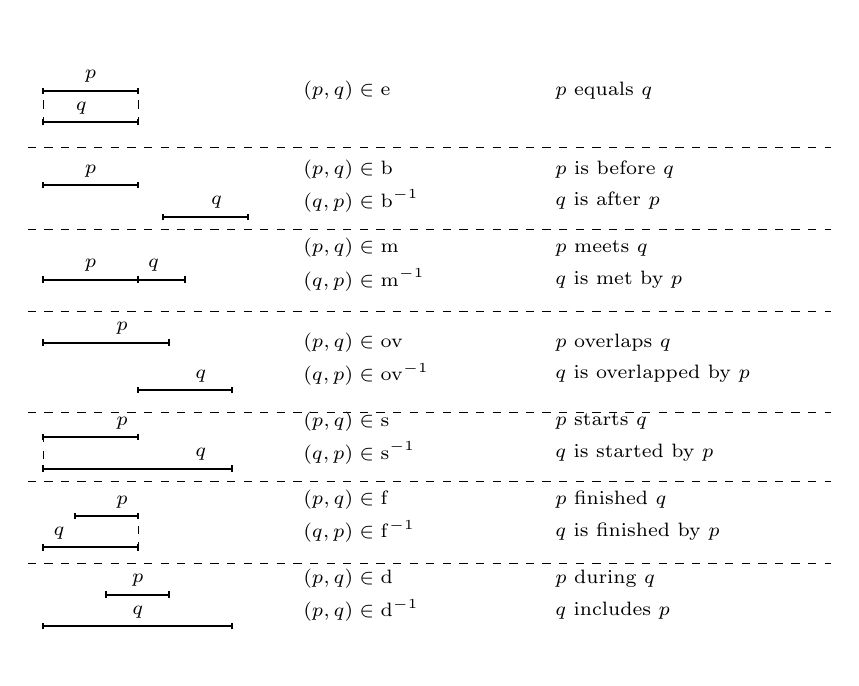
\begin{tikzpicture}[x=.5cm,y=.5cm, scale =0.8]
\clip(-0.5,-16) rectangle (25,4);
\scriptsize
% (p,q) : e
\draw [line width = 0.7pt] (0,2) -- (3,2);
\draw[line width = 0.7pt] (0,1.9) -- (0,2.1);
\draw[line width = 0.7pt] (3,1.9) -- (3,2.1);
\node [above] at (1.5,2) { $p$};
\draw [line width = 0.7pt] (0,1) -- (3,1);
\draw [line width = 0.7pt] (0,0.9) -- (0,1.1);
\draw [line width = 0.7pt] (3,0.9) -- (3,1.1);
\node [above ] at (1.2, 1) { $q$};
\draw [line width = 0.2pt, dashed] (0,0.9) -- (0,1.9);
\draw [line width = 0.2pt, dashed] (3,0.9) -- (3,2.1);


\node [right] at (8,2) {$(p,q) \in \mathrm{e}$};
\node [right] at (16,2) {$p$ {equals} $q$};

\draw[line width= 0.2pt, dashed] (-0.5,0.2) -- (25,0.2);
% (p,q) : b
\draw [line width = 0.7pt] (0,-1) -- (3,-1);
\draw[line width = 0.7pt] (0,-1.1) -- (0,-0.9);
\draw[line width = 0.7pt] (3,-1.1) -- (3,-0.9);
\node [above] at (1.5,-1) { $p$};
\draw [line width = 0.7pt] (3.8,-2) -- (6.5,-2);
\draw [line width = 0.7pt] (3.8,-2.1) -- (3.8,-1.9);
\draw [line width = 0.7pt] (6.5,-2.1) -- (6.5,-1.9);
\node [above] at (5.5,-2) { $q$};
\node [right] at (8,-0.5) {$(p,q) \in \mathrm{b}$};
\node [right] at (16,-0.5) {$p$ {is before} $q$};
\node [right] at (8,-1.5) {$(q,p) \in \mathrm{b}^{-1}$};
\node [right] at (16,-1.5) {$q$ {is after} $p$};

\draw[line width= 0.2pt, dashed] (-0.5,-2.4) -- (25,-2.4);

% (p,q) : m
\draw [line width = 0.7pt] (0,-4) -- (3,-4);
\draw [line width = 0.7pt] (0,-4.1) -- (0,-3.9);
\draw [line width = 0.7pt] (3,-4.1) -- (3,-3.9);
\node [above] at (1.5,-4) { $p$};
\draw [line width = 0.7pt] (3,-4) -- (4.5,-4);
\draw [line width = 0.7pt] (4.5,-4.1) -- (4.5,-3.9);
\node [above] at (3.5,-4) { $q$};
\node [right] at (8,-3) {$(p,q) \in \mathrm{m}$};

\node [right] at (8,-4) {$(q,p) \in \mathrm{m}^{-1}$};
\node [right] at (16,-3) {$p$ {meets} $q$};
\node [right] at (16,-4) {$q$ {is met by} $p$};

\draw[line width= 0.2pt, dashed] (-0.5,-5) -- (25,-5);

% (p,q) : ov
\draw [line width = 0.7pt] (0,-6) -- (4,-6);
\draw [line width = 0.7pt] (0,-6.1) -- (0,-5.9);
\draw [line width = 0.7pt] (4,-6.1) -- (4,-5.9);
\node [above] at (2.5,-6) { $p$};
\draw [line width = 0.7pt] (3,-7.5) -- (6,-7.5);
\draw [line width = 0.7pt] (3,-7.6) -- (3,-7.4);
\draw [line width = 0.7pt] (6,-7.6) -- (6,-7.4);
\node [above] at (5,-7.5) { $q$};
\node [right] at (8,-6) {$(p,q) \in \mathrm{ov}$};

\node [right] at (8,-7) {$(q,p) \in \mathrm{ov}^{-1}$};
\node [right] at (16,-6) {$p$ overlaps $q$};
\node [right] at (16,-7) {$q$ {is overlapped by} $p$};

\draw[line width = 0.2pt, dashed] (-0.5, -8.2) -- (25,-8.2);

% (p,q) : s
\draw [line width = 0.7pt] (0,-9) -- (3,-9);
\draw [line width = 0.7pt] (0,-9.1) -- (0,-8.9);
\draw [line width = 0.7pt] (3,-9.1) -- (3,-8.9);
\node [above] at (2.5,-9) { $p$};
\draw [line width = 0.7pt] (0,-10) -- (6,-10);
\draw [line width = 0.7pt] (0,-10.1) -- (0,-9.9);
\draw [line width = 0.7pt] (6,-10.1) -- (6,-9.9);
\node [above] at (5,-10) { $q$};

\draw[line width = 0.2pt, dashed] (0,-8.9) -- (0,-10.1);
\node [right] at (8,-8.5) {$(p,q) \in \mathrm{s}$};

\node [right] at (8,-9.5) {$(q,p) \in \mathrm{s}^{-1}$};
\node [right] at (16,-8.5) {$p$ starts $q$};
\node [right] at (16,-9.5) {$q$ {is started by} $p$};

\draw[line width = 0.2pt, dashed] (-0.5, -10.4) -- (25,-10.4);

% (p,q) :f

\draw [line width = 0.7pt] (1,-11.5) -- (3,-11.5);
\draw [line width = 0.7pt] (1,-11.6) -- (1,-11.4);
\draw [line width = 0.7pt] (3,-11.6) -- (3,-11.4);
\node [above] at (2.5,-11.5) { $p$};
\draw [line width = 0.7pt] (0,-12.5) -- (3,-12.5);
\draw [line width = 0.7pt] (0,-12.6) -- (0,-12.4);
\draw [line width = 0.7pt] (3,-12.6) -- (3,-12.4);
\node [above] at (0.5,-12.5) { $q$};

\draw[line width = 0.2pt, dashed] (3,-12.6) -- (3,-11.4);
\node [right] at (8,-11) {$(p,q) \in \mathrm{f}$};

\node [right] at (8,-12) {$(q,p) \in \mathrm{f}^{-1}$};
\node [right] at (16,-11) {$p$ finished $q$};
\node [right] at (16,-12) {$q$ {is finished by} $p$};

\draw[line width = 0.2pt, dashed] (-0.5, -13) -- (25,-13);

% (p,q) :d

\draw [line width = 0.7pt] (2,-14) -- (4,-14);
\draw [line width = 0.7pt] (2,-14.1) -- (2,-13.9);
\draw [line width = 0.7pt] (4,-14.1) -- (4,-13.9);
\node [above] at (3,-14) { $p$};
\draw [line width = 0.7pt] (0,-15) -- (6,-15);
\draw [line width = 0.7pt] (0,-15.1) -- (0,-14.9);
\draw [line width = 0.7pt] (6,-15.1) -- (6,-14.9);
\node [above] at (3,-15) { $q$};
\node [right] at (8,-13.5) {$(p,q) \in \mathrm{d}$};

\node [right] at (8,-14.5) {$(p,q) \in \mathrm{d}^{-1}$};
\node [right] at (16,-13.5) {$p$ during $q$};
\node [right] at (16,-14.5) {$q$ {includes} $p$};
\end{tikzpicture}
\caption{The 13 time interval relations}
\label{fig:arels}
\end{figure}
%
%The day to day conversation involves the relative occurrence of events, which is the qualitative information on times of events.  For instance, let's consider the following statement by a student.
%\begin{quote}
%``Today, I attended algebra (A) and programming (P) classes. Algebra class was too long and overlapped with my lunch."
%\end{quote} 
%can be represented by the following relations on time intervals.
%\begin{align*}
%&
% \text{(A, P) }\in (m, m^{-1}, b, b^{-1}) \\
%& 
%\text{(A, L) }\in  ov %\\
%%& \text{(L, P) }\in  \; ? \\
%%& \text{(presentation, programming) }\in \{d, s, f\}.
%\end{align*}
%Allen introduced 13 binary relations that define all the possible qualitative arrangements that can exist between two time intervals~\cite{Allen:1983}. These relations cover basic situations of two events in the sense they can be equal, before, meeting, starting, finishing, overlapping or during each other. These relations represent qualitative information in the sense that they use notion of time in day to day conversation where we are  concerned with the relative occurrence of events rather than the exact time and duration. Figure \ref{fig:arels} depicts the 13 time interval relations. %Events are represented qualitatively as intervals together with binary relations. Relations e, m, b, ov, d, s and f stand for equal, meets, before, overlaps, during, starts and finishes, respectively.  
%The following statement  by a students is qualitatively represented by relation constraints in Fig.~\ref{fig:graph}
%
%
%
%%``This morning, I attend a class of mathematical logic then a class of algebra. Algebra class was long and took 10 minutes of my lunch. Later, I present my homework during programming class." 
%\begin{quote}``Today, I attended two classes: algebra (A) and programming (P). Algebra class was too long and overlapped with my lunch (L)." \end{quote}
%
%\begin{align*}
%&
% \text{(A, P) }\in (m, m^{-1}, b, b^{-1}) \\
%& 
%\text{(A, L) }\in  ov %\\
%%& \text{(L, P) }\in  \; ? \\
%%& \text{(presentation, programming) }\in \{d, s, f\}.
%\end{align*}
%
%\begin{figure}
%%\centering
%%\subfloat[]{\parbox{3cm}{\begin{align*}
%%&
%% \text{(A, P) }\in \{m, m^{-1}, b, b^{-1}\} \\
%%& 
%%\text{(A, L) }\in \{ ov \} %\\
%%%& \text{(L, P) }\in  \; ? \\
%%%& \text{(presentation, programming) }\in \{d, s, f\}.
%%\end{align*}}}
%{\begin{tikzpicture}[line cap=round,line join=round,>=triangle 45,x=1.0cm,y=1.0cm, scale = 1]
%\clip(-3,0) rectangle (6,6);
%%\tikzstyle{every node}=[draw,shape=circle,fill=gray!6];
%\node (A) at (0.9,2) [circle] {A};
%\node (P) at (3,5)  {P};
%\node (L) at (4,1)  {L};
%\begin{graph}
%{(P) -> [edge label={\tiny (m, m$^{-1}$, b , b$^{-1}$)}, swap] (A)
%(A) -> [edge label={\tiny ov}, swap] (L)};
%%(L) -> [edge label={\tiny ov}, swap] (L)} ;
%\end{graph}
%%\draw (A) edge [->] (P) {\{m, m$^{-1}, b , b$^{-1}$\}};
%\end{tikzpicture}}
%\caption{Interval time relation graph constraints}
%\label{fig:graph}
%\end{figure}
%
%\begin{itemize}
%\item We can deduce new relation
%\begin{align}
%& \text{(A, P) }\in (m, m^{-1}, b, b^{-1}), \\
%& \text{(A, L) }\in  ov,  \\
%& \text{(L, P) }\in  \; ? \\
%%& \text{(presentation, programming) }\in \{d, s, f\}.
%\end{align}
%\item Check consistency of relation constraints
% \begin{align}
%& \text{(A, P) }\in (m, m^{-1}, b, b^{-1}), \\
%& \text{(A, L) }\in ov, \\
%& \text{(L, P) }\in  m \\
%%& \text{(presentation, programming) }\in \{d, s, f\}.
%\end{align}
%\item Construct an algebraically closed scenario
% \begin{align}
%& \text{(A, P) }\in b, \\
%& \text{(A, L) }\in ov, \\
%& \text{(L, P) }\in  m \\
%%& \text{(presentation, programming) }\in \{d, s, f\}.
%\end{align}
%\end{itemize}
%\tikz { \graph { Alg [circle] -> [bend right, "\{m, m$^{-1}$, b, b$^{-1}$\}"] ML;};}
%\begin{itemize}
%\item Introducing qualitative reasoning to automated reasoning community
%\item The state-of-art of theorem proving in QR:
%\begin{itemize}
%\item Shulz's algebraic constraint solving to provide an automated proof of consistency, correctness of composition tables.
%\item Interactive proofs by OTTER that cover the composition table of RCC
%\end{itemize}
%\item We focus on Allen's interval algebra. We formalize the axiom system and define the time relations in Isabelle/HOL. We discuss proof strategies to tackle the correctness of composition tables.
%\item Relations e, m, b, ov, d, s and f stand for equal, meets, before, overlaps, during, starts and finishes, respectively. Figure \ref{fig:arels} shows a geometric representation of the 7 relations and their converses(13 relations in total). 
%\item Isabelle/HOL
%\item Significance: composition tables are important to decide the consistency of qualitative constraints.
%\end{itemize}








%\draw[line width = 0.2pt, dashed] (-0.5, -12.9) -- (25,-12.9);


% \end{figure}
%\begin{figure}[h]
%\centering
%\subfloat[$(p,q) \in e$: time intervals $p$ and $q$ are equal ]{\begin{tikzpicture}[line cap=round,line join=round,>=triangle 45,x=1.0cm,y=1.0cm, scale = 0.5]
%\clip(-1,-0.8) rectangle (6,2);
%\draw [line width = 0.7pt] (0,1) -- (3,1);
%\node [above] at (1.5,1) { $p$};
%\draw [line width = 0.7pt] (0,0) -- (3,0);
%\node [above] at (1.5,0) { $q$};
%\end{tikzpicture}}\quad
%\subfloat[$(p,q) \in b$: $p$ is \textit{before} $q$,\qquad  $(q,p)\in b^{-1}$: $q$ is \textit{after} $p$]
%{\begin{tikzpicture}[line cap=round,line join=round,>=triangle 45,x=1.0cm,y=1.0cm, scale = 0.5]
%\clip(-1,-0.8) rectangle (8,2);
%\draw [line width = 0.7pt] (0,1) -- (3,1);
%\node [above] at (1.5,1) { $p$};
%\draw [line width = 0.7pt] (3.8,0) -- (6.5,0);
%\node [above] at (5.5,0) { $q$};
%\end{tikzpicture}}\quad
%\subfloat[$(p,q) \in m$: $p$ \textit{meets} $q$,\qquad $(q,p) \in m^{-1}$: $q$ \textit{meets-by} $p$]{\begin{tikzpicture}[line cap=round,line join=round,>=triangle 45,x=1.0cm,y=1.0cm, scale = 0.5]
%\clip(-1,-0.8) rectangle (8,2);
%\draw [line width = 0.7pt] (0,1) -- (3,1);
%\node [above] at (1.5,1) { $p$};
%\draw [line width = 0.7pt] (3,0) -- (6,0);
%\node [above] at (5,0) { $q$};
%\draw [line width = 0.7pt, dashed] (3,1.2) -- (3,-0.8);
%\end{tikzpicture}}
%\subfloat[$(p,q) \in s$: $p$ \textit{starts at} $q$, \qquad $(q,p) \in s^{-1}$: $q$ \textit{started by} $p$]{\begin{tikzpicture}[line cap=round,line join=round,>=triangle 45,x=1.0cm,y=1.0cm, scale = 0.5]
%\clip(-1,-0.8) rectangle (8,2);
%\draw [line width = 0.7pt] (0,1) -- (3,1);
%\node [above] at (1.5,1) { $p$};
%\draw [line width = 0.7pt] (0,0) -- (6,0);
%\node [above] at (5,0) { $q$};
%\draw [line width = 0.7pt, dashed] (0,1.2) -- (0,-0.8);
%\end{tikzpicture}}
%\subfloat[$(p,q) \in f$: $p$ \textit{finishes} at $q$, $(q,p) \in f^{-1}$: $q$ \textit{finishes by} $p$]{\begin{tikzpicture}[line cap=round,line join=round,>=triangle 45,x=1.0cm,y=1.0cm, scale = 0.5]
%\clip(-1,-0.8) rectangle (8,2);
%\draw [line width = 0.7pt] (4,1) -- (6,1);
%\node [above] at (5,1) { $p$};
%\draw [line width = 0.7pt] (0,0) -- (6,0);
%\node [above] at (3,0) { $q$};
%\draw [line width = 0.7pt, dashed] (6,1.2) -- (6,-0.8);
%\end{tikzpicture}}
%\subfloat[$(p,q) \in d$: $p$ happens \textit{during} $q$, \qquad $(q,p) \in d^{-1}$: $q$ \textit{includes} $p$]{\begin{tikzpicture}[line cap=round,line join=round,>=triangle 45,x=1.0cm,y=1.0cm, scale = 0.5]
%\clip(-1,-0.8) rectangle (8,2);
%\draw [line width = 0.7pt] (3.6,1) -- (5,1);
%\node [above] at (4.5,1) { $p$};
%\draw [line width = 0.7pt] (0,0) -- (6,0);
%\node [above] at (3,0) { $q$};
%%\draw [line width = 0.7pt, dashed] (6,1.2) -- (6,-0.8);
%\end{tikzpicture}}
%\subfloat[$(p,q) \in ov$: $p$ \textit{overlaps} $q$, \qquad $(q,p)\in ov^{-1}$: $q$ is \textit{overlapped by} $p$]{\begin{tikzpicture}[line cap=round,line join=round,>=triangle 45,x=1.0cm,y=1.0cm, scale = 0.5]
%\clip(-1,-0.8) rectangle (9,2);
%\draw [line width = 0.7pt] (0,1) -- (4,1);
%\node [above] at (2.5,1) { $p$};
%\draw [line width = 0.7pt] (3,0) -- (6,0);
%\node [above] at (5,0) { $q$};
%%\draw [line width = 0.7pt, dashed] (6,1.2) -- (6,-0.8);
%\end{tikzpicture}}
%\caption{The 13 time interval relations}
%\label{fig:arels}
%\end{figure}
%\section{ALLEN INTERVAL CALCULUS}
%\subsection{JEPD relations}
%Allen defines 13 relations of between time intervals. They establish relations between intervals of time. 
%\subsection{Composition of time interval relations}
%\section{Relation Algebra}

%Relation.converse_iff: ((?a, ?b) ? ?r¯) = ((?b, ?a) ? ?r)
%\section{Preliminaries \textcolor{red}{too short, move somewhere in the text}}
%\label{sect:prem}
%

\section{Basic Relations}
\label{sect:brel}


An event is continuous in a finite period of time. An event is qualitatively represented as a time interval, and  the basic objects that we consider in our formalization are  intervals. %It is arguable whether points are necessary since they can represent instantaneous events. We agree with Allen that intervals are what we need to reason about a class of knowledge on time. 
For simplicity (and like most papers on Allen's calculus), we illustrate our explanation with a spatial representation of intervals as parallel line segments. Moreover,  the notions of ``starting point" and ``ending point" of intervals- although not formally defined- support our explanation. % in the following sections. 

There are  13 possible arrangements of time intervals. They can be described with relations {before}, {equal}, {starting}, {finishing}, {overlapping}, {meeting} or {during}. %The arrangements of two time intervals are described in . 
The relations together with their respective inverses are 13 and they are depicted in Fig.~\ref{fig:arels}. Hereafter, relations before, meets, overlaps, starts, finishes, during and equal are abbreviated to \texttt{b}, \texttt{m}, \texttt{ov}, \texttt{s}, \texttt{f}, \texttt{d} and \texttt{e}, respectively. 

When the relation between two events is completely known, then it is represented with one of the 13 time interval relations that we call \textit{basic} relations. For example, the statement  ``Tarski (T) lived after Euclid (E)."  unambiguously expresses that Euclid's life preceded Tarski's life, which can be represented (T, E) $\in$ \texttt{b}$^{-1}$ (or (E, T) $\in$ \texttt{b}). 

Sometimes, the knowledge is not precise. The statement ``Hilbert (H) was born before Tarski (T)." lacks information about who died first and whether one was born after the death of the other, etc.  Nevertheless, we still can  represent these various situations as follows (H, T) $\in$ \texttt{b} $\cup$ \texttt{ov} $\cup$ \texttt{m} $\cup$ \texttt{d}$^{-1}$ $\cup$ \texttt{f}$^{-1}$, i.e.~the life of Hilbert is either before or overlaps or meets or includes or finishes by the life of Tarski. We can derive new qualitative knowledge by composing relations. The relation (H, E) is the composition of relations  \texttt{b} $\cup$ \texttt{ov} $\cup$ \texttt{m} $\cup$ \texttt{d}$^{-1}$ $\cup$ \texttt{f}$^{-1}$ and \texttt{b}$^{-1}$.

For simplicity, $(r_1, \ldots, r_n)$ denotes the union of basic relations $r_1, \ldots, r_n$. Thus, $x \in (r_1, \ldots, r_n)$ is equivalent to $x \in r_1 \lor \ldots \lor  x \in r_n$. Let $\alpha_1 = (r_1, \ldots, r_i)$ and $\alpha_2 = (r_1', \ldots, r_j')$, we denote by $\alpha_1 + \alpha_2$ the union $(r_1, \ldots, r_i, r_1', \ldots, r_j')$. %of relations $r_1, \ldots, r_i, r_1', \ldots, r_j'$, i.e.~$\alpha_1 + \alpha_2 = (r_1, \ldots, r_i, r_1', \ldots, r_j')$. 



\section{Axioms}
\label{sect:axioms}
%\subsection{Interval of Time}
%An event continues for a finite period of time. An event is qualitatively represented as time interval and thus the basic object that we consider in our formalization is an interval. It is arguable whether points are necessary since they can represent instantaneous events. We are faithful to the original calculus defined by Allen. The notions of ``starting point" and ``ending point" of intervals- although not formally defined- are useful in our intuitive explanation of the axioms and time relations in the following sections. 
%with a starting time and ending time. The temporal object that we use is interval. 
%\subsection{The Axiom Set}
%An event is continuous in a finite period of time. An event is qualitatively represented as a time interval, and  the basic objects that we consider in our formalization are  intervals. %It is arguable whether points are necessary since they can represent instantaneous events. We agree with Allen that intervals are what we need to reason about a class of knowledge on time. 
%For simplicity (and like most papers on Allen's calculus), we illustrate our explanation with a spatial representation of intervals as parallel line segments. Moreover,  the notions of ``starting point" and ``ending point" of intervals- although not formally defined- are useful in our intuitive explanation. % in the following sections. 

We consider the situations where two time intervals can be equal or meeting each other. Equality between interval is an equivalence relation. Two intervals meet if one interval ends at the starting time of the second.  The intervals are therefore  adjacent. For instance in Fig.~\ref{fig:meets}, interval $p$ meets interval $q$. The meets relation is irreflexive, non-symmetric and non-transitive. A set of five axioms (M1) $\sim$ (M5) is then defined based on equality and relation meets. 
\begin{figure}[h]
\centering
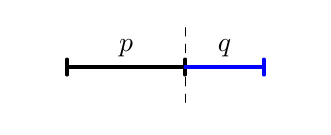
\begin{tikzpicture}[line cap=round,line join=round,>=triangle 45,x=1.0cm,y=1.0cm, scale = 0.5]
\clip(-1,0) rectangle (6,2);

\node [above] at (1.5,1) { $p$};
\draw [black, line width = 1.2pt ] (0,1) -- (3,1);
\draw [black , line width = 1.2pt ] (0,1.2) -- (0,0.8);
\draw [black , line width = 1.2pt ] (3,1.2) -- (3,0.8);
\draw [dashed ] (3,2) -- (3,0);

\node [above] at (4,1) { $q$};
\draw [blue, line width = 1.2pt  ] (3,1) -- (5,1);
\draw [blue, line width = 1.2pt  ] (5,1.2) -- (5,0.8);

%\draw [black, dashed ] (3,1.4) -- (3,0.6);
\end{tikzpicture}
\caption{Interval $p$ meets interval $q$}
\label{fig:meets}
\end{figure}

%We use Isabelle/HOL's equality relation for interval equality. 
We define a class type interval whose assumptions are (a) properties of relation meets, denoted by the infix symbol ``$||$" and, (b) axioms (M1) $\sim$ (M5). %We use Isabelle/HOL's equality relation for interval equality. %We choose type class because an interpretation of time interval is an instance of class interval that should satisfy the set of axioms.
\begin{isabellebody}
\small\isanewline
\isacommand{class}\isamarkupfalse%
\ interval\ {\isacharequal}\isanewline
\ \isakeyword{fixes}\isanewline
\ \ meets{\isacharcolon}{\isacharcolon}{\isachardoublequoteopen}{\isacharprime}a\ {\isasymRightarrow}\ {\isacharprime}a\ {\isasymRightarrow}\ bool{\isachardoublequoteclose}\ \ {\isacharparenleft}\isakeyword{infixl}\ {\isachardoublequoteopen}{\isasymparallel}{\isachardoublequoteclose}\ {\isadigit{6}}{\isadigit{0}}{\isacharparenright}\ \isanewline
\ \isakeyword{assumes}\isanewline
\ \ meets{\isacharunderscore}atrans{\isacharcolon}{\isachardoublequoteopen}{\isasymlbrakk}p{\isasymparallel}q {\isacharsemicolon}  q{\isasymparallel}r{\isasymrbrakk}\ {\isasymLongrightarrow}\ {\isasymnot}{\isacharparenleft}p{\isasymparallel}r{\isacharparenright}{\isachardoublequoteclose}\ \isakeyword{and}\isanewline
\ \ meets{\isacharunderscore}irrefl{\isacharcolon}{\isachardoublequoteopen}{\isasymnot}{\isacharparenleft}p{\isasymparallel}p{\isacharparenright}{\isachardoublequoteclose}\ \isakeyword{and}\isanewline
\ \ meets{\isacharunderscore}asym{\isacharcolon}{\isachardoublequoteopen}p{\isasymparallel}q\ {\isasymLongrightarrow}\ {\isasymnot}{\isacharparenleft}q{\isasymparallel}p{\isacharparenright}{\isachardoublequoteclose}\ \isakeyword{and}\isanewline
%\ \ eq{\isacharunderscore}refl{\isacharcolon}{\isachardoublequoteopen}p\ {\isacharequal}\  p{\isachardoublequoteclose}\ \isakeyword{and}\ \isanewline
%\ \ eq{\isacharunderscore}sym{\isacharcolon}{\isachardoublequoteopen}{\isacharparenleft}p\ {\isacharequal}\ q{\isacharparenright}\ {\isacharequal}\ {\isacharparenleft}q\ {\isacharequal}\ p{\isacharparenright}{\isachardoublequoteclose}\ \isakeyword{and}\ \isanewline
%\ \ eq{\isacharunderscore}tran{\isacharcolon}{\isachardoublequoteopen}{\isasymlbrakk}p\ {\isacharequal}\ q {\isacharsemicolon}\ q\ {\isacharequal}\ r {\isasymrbrakk}\ {\isasymLongrightarrow}\ {\isacharparenleft}p\ {\isacharequal}\ r{\isacharparenright}{\isachardoublequoteclose}\ \isakeyword{and}\isanewline
%\isanewline
\ \ M{\isadigit{1}}{\isacharcolon}{\isachardoublequoteopen}{\isasymlbrakk}p{\isasymparallel}q{\isacharsemicolon}\ p{\isasymparallel}s{\isacharsemicolon}\ r{\isasymparallel}q{\isasymrbrakk}\ {\isasymLongrightarrow}\ {\isacharparenleft}r{\isasymparallel}s{\isacharparenright}{\isachardoublequoteclose}\ \isakeyword{and}\isanewline
\ \ M{\isadigit{2}}{\isacharcolon}{\isachardoublequoteopen}{\isasymlbrakk}p{\isasymparallel}q {\isacharsemicolon}\  r{\isasymparallel}s{\isasymrbrakk}\ {\isasymLongrightarrow} \isanewline \ \ \ \ \ \ \ \ \ \ \ \  \ \ \ p{\isasymparallel}s\ {\isasymoplus}\ {\isacharparenleft}{\isacharparenleft}{\isasymexists}t{\isachardot}\ {\isacharparenleft}p{\isasymparallel}t{\isacharparenright}{\isasymand}{\isacharparenleft}t{\isasymparallel}s{\isacharparenright}{\isacharparenright}\ {\isasymoplus}\ {\isacharparenleft}{\isasymexists}t{\isachardot}\ {\isacharparenleft}r{\isasymparallel}t{\isacharparenright}{\isasymand}{\isacharparenleft}t{\isasymparallel}q{\isacharparenright}{\isacharparenright}{\isacharparenright}{\isachardoublequoteclose}\ \isakeyword{and}\isanewline
\ \ M{\isadigit{3}}{\isacharcolon}{\isachardoublequoteopen}{\isacharparenleft}{\isasymexists}q\ r{\isachardot}\ q{\isasymparallel}p\ {\isasymand}\ p{\isasymparallel}r{\isacharparenright}{\isachardoublequoteclose}\ \isakeyword{and}\isanewline
\ \ M{\isadigit{4}}{\isacharcolon}{\isachardoublequoteopen}{\isasymlbrakk}p{\isasymparallel}q\ {\isacharsemicolon}\ q{\isasymparallel}s\ {\isacharsemicolon}\ p{\isasymparallel}r\ {\isacharsemicolon}\ r{\isasymparallel}s{\isasymrbrakk}\ {\isasymLongrightarrow}\ q\ {\isacharequal}\ r{\isachardoublequoteclose}\ \ \isakeyword{and}\isanewline
\ \ M{\isadigit{5}}exist{\isacharcolon}{\isachardoublequoteopen}p{\isasymparallel}q\ {\isasymLongrightarrow}\ {\isacharparenleft}{\isasymexists}r\ s\ t{\isachardot}\ r{\isasymparallel}p\ {\isasymand}\ p{\isasymparallel}q\ {\isasymand}\ q{\isasymparallel}s\ {\isasymand}\ r{\isasymparallel}t\ {\isasymand}\ t{\isasymparallel}s{\isacharparenright}{\isachardoublequoteclose}\isanewline
\end{isabellebody}

%Hereafter, we explain the axioms (M1) $\sim$ (M5) referring to Fig.~\ref{fig:M1M5}. % and how they are relevant in a constructive-style proof. For simplicity, we explain the axioms in an intuitive understanding of time where an interval is parallel to a horizontal line, and has a starting instant and an ending instant.

Figures \ref{fig:M1M5} and \ref{fig:M2} illustrate the five time interval axioms:
\begin{itemize}
\item Axiom (M1) uniquely defines the meeting point of two intervals. If two intervals $p$ and $r$ meet the same interval, then $r$ meets any interval that $p$ meets. % (c.f.~Fig.\ref{}).
\item Axiom (M3) states that for any interval $p$ there is an interval that meets $p$ and an interval that it meets, which means there a time interval does not last infinitly.
\item Axiom (M4) states that an interval is uniquely defined by the starting and the ending point. 
\item Axiom (M5) states that the addition of two intervals that meet is an intervals. %We deduce the addition of three intervals. 
\item Axiom (M2) takes two pairs of intervals that meet in two points, and states that  either the meeting points are equal or one of them precedes the other.  Axiom (M2) states that the three configurations are mutually exclusive, i.e. not more than one can hold, and exhaustive, i.e. at least one of the three must hold.
\end{itemize}

\begin{figure}[h]
\scriptsize
\centering
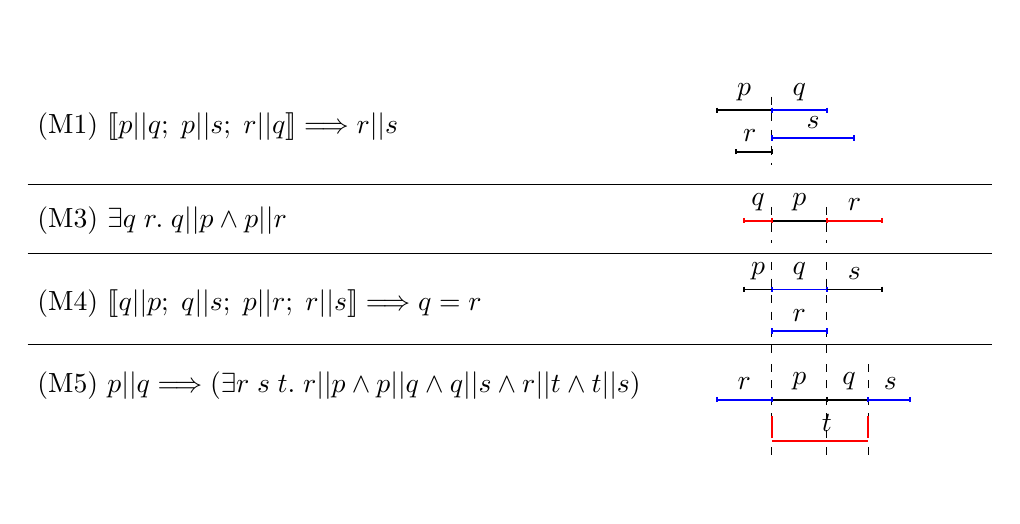
\begin{tikzpicture}[x=.5cm,y=.5cm, scale =0.7]
\clip(-25,6) rectangle (10,23);

% ------- (M1) --------
\draw [line width = 0.7pt] (0,20) -- (2,20);
\draw [line width = 0.7pt] (0,20.1) -- (0,19.9);
\draw [line width = 0.7pt] (2,20.1) -- (2,19.9);

\node [above] at (1,20) { $p$};
\draw [black, dashed ] (2,20.5) -- (2,18);
\draw [line width = 0.7pt, blue] (2,20) -- (4,20);
\draw [line width = 0.7pt, blue] (2,20.1) -- (2,19.9);
\draw [line width = 0.7pt, blue] (4,20.1) -- (4,19.9);
\node [above] at (3,20) { $q$};
%-- s
\draw [line width = 0.7pt, blue] (2,19) -- (5,19);
\draw [line width = 0.7pt, blue] (2,19.1) -- (2,18.9);
\draw [line width = 0.7pt,blue] (5,19.1) -- (5,18.9);

\node [above] at (3.5,19) { $s$};

%-- r
\draw [line width = 0.7pt] (0.7,18.5) -- (2,18.5);
\draw [line width = 0.7pt] (0.7,18.4) -- (0.7,18.6);
\draw [line width = 0.7pt] (2,18.4) -- (2,18.6);
\node [above] at (1.2,18.5) { $r$};

\node [right] at (-25, 19.4) {(M1) $\llbracket p||q;\; p||s ; \; r||q\rrbracket \Longrightarrow r||s$};
\draw[line width=0.2pt] (-25,17.3) -- (10,17.3);
% ------- (M3) --------
\draw [line width = 0.7pt] (2,16) -- (4,16);

\node [above] at (3,16) { $p$};
\draw [black, dashed ] (2,16.5) -- (2,15.2);
\draw [black, dashed ] (4,16.5) -- (4,15.2);

%-- q
\draw [line width = 0.7pt, red] (1,16) -- (2,16);
\draw [line width = 0.7pt, red] (2,16.1) -- (2,15.9);
\draw [line width = 0.7pt, red] (1,16.1) -- (1,15.9);

\node [above] at (1.5,16) { $q$};

%-- r
\draw [line width = 0.7pt, red] (4,16) -- (6,16);
\draw [line width = 0.7pt, red] (4,16.1) -- (4,15.9);
\draw [line width = 0.7pt, red] (6,16.1) -- (6,15.9);

\node [above] at (5,16) { $r$};
\node [right] at (-25, 16) {(M3) $\exists q\; r. \; q||p \land p||r$};
\draw[line width = 0.2pt] (-25,14.8) -- (10,14.8);

%-------- (M4) --------
\draw [line width = 0.7pt, blue] (2,13.5) -- (4,13.5);
\draw [line width = 0.7pt, blue] (2,13.6) -- (2,13.4);
\draw [line width = 0.7pt, blue] (4,13.6) -- (4,13.4);

\node [above] at (3,13.5) { $q$};
\draw [black, dashed ] (2,14.5) -- (2,11.2);
\draw [black, dashed ] (4,14.5) -- (4,11.2);

%-- p
\draw [line width = 0.7pt] (1,13.5) -- (2,13.5);
\draw [line width = 0.7pt] (1,13.6) -- (1,13.4);

\node [above] at (1.5,13.5) { $p$};

%-- s
\draw [line width = 0.7pt] (4,13.5) -- (6,13.5);
\draw [line width = 0.7pt] (6,13.6) -- (6,13.4);

\node [above] at (5,13.5) { $s$};

%-- r
\draw [line width = 0.7pt, blue] (2,12) -- (4,12);
\draw [line width = 0.7pt, blue] (2,12.1) -- (2,11.9);
\draw [line width = 0.7pt, blue] (4,12.1) -- (4,11.9);

\node [above] at (3,12) { $r$};
\node [right] at (-25, 13) {(M4) $\llbracket q||p ;\; q||s; \; p||r ;\; r||s\rrbracket \Longrightarrow q = r$};
\draw[line width = 0.2pt] (-25,11.5) -- (10,11.5);

%-------- (M5) -------
\draw [line width = 0.7pt] (2,9.5) -- (4,9.5);
\draw [line width = 0.7pt] (4,9.6) -- (4,9.4);

\node [above] at (3,9.5) { $p$};
\draw [line width = 0.7pt] (4,9.5) -- (5.5,9.5);
\node [above] at (4.8,9.5) { $q$};
\draw [black, dashed ] (2,7.5) -- (2,11);
\draw [black, dashed ] (4,7.5) -- (4,11);
\draw [black, dashed ] (5.5,7.5) -- (5.5,11);

%--- r 
\draw [line width = 0.7pt, blue] (0,9.5) -- (2,9.5);
\draw [line width = 0.7pt, blue] (0,9.6) -- (0,9.4);
\draw [line width = 0.7pt, blue] (2,9.6) -- (2,9.4);

\node [above] at (1,9.5) { $r$};

%--- s
\draw [line width = 0.7pt, blue] (5.5,9.5) -- (7,9.5);
\draw [line width = 0.7pt, blue] (5.5,9.4) -- (5.5,9.6);
\draw [line width = 0.7pt, blue] (7,9.4) -- (7,9.6);

\node [above] at (6.3,9.5) { $s$};

%--- t
\draw [line width = 0.7pt, red] (2,8) -- (5.5,8);
\draw [line width = 0.7pt, red] (2,8.9) -- (2,8.1);
\draw [line width = 0.7pt, red] (5.5,8.9) -- (5.5,8.1);

\node [above] at (4,8) { $t$};
\node [right] at (-25, 10) {(M5) $ p||q \Longrightarrow (\exists r\;s\;t. \;r||p\land p||q \land q||s \land r||t \land t||s)$};
\end{tikzpicture}
\caption{Axioms (M1), (M3) $\sim$ (M5)}
\label{fig:M1M5}
\end{figure}


%\begin{figure}
%\centering
%\subfloat[Axiom (M1)]{
%\begin{tikzpicture}[line cap=round,line join=round,>=triangle 45,x=1.0cm,y=1.0cm, scale = 0.38]
%\clip(-1,-2) rectangle (8.5,2);
%\draw [->] (-1,-1 ) -- (6, -1);
%\node [right] at (6, -1) {\tiny time};
%\draw [line width = 0.7pt] (0,1) -- (2,1);
%\draw [line width = 0.7pt] (0,1.1) -- (0,0.9);
%\draw [line width = 0.7pt] (2,1.1) -- (2,0.9);
%
%\node [above] at (1,1) { $p$};
%\draw [black, dashed ] (2,1.5) -- (2,-1.2);
%\draw [line width = 0.7pt, blue] (2,1) -- (4,1);
%\draw [line width = 0.7pt, blue] (2,1.1) -- (2,0.9);
%\draw [line width = 0.7pt, blue] (4,1.1) -- (4,0.9);
%\node [above] at (3,1) { $q$};
%%-- s
%\draw [line width = 0.7pt, blue] (2,0) -- (5,0);
%\draw [line width = 0.7pt, blue] (2,0.1) -- (2,-0.1);
%\draw [line width = 0.7pt,blue] (5,0.1) -- (5,-0.1);
%
%\node [above] at (3.5,0) { $s$};
%
%%-- r
%\draw [line width = 0.7pt] (0.7,-0.5) -- (2,-0.5);
%\draw [line width = 0.7pt] (0.7,-0.4) -- (0.7,-0.6);
%\draw [line width = 0.7pt] (2,-0.4) -- (2,-0.6);
%\node [above] at (1.2,-0.5) { $r$};
%
%\end{tikzpicture}\label{fig:M1}
%}\quad
%\subfloat[Axiom (M3)]{
%\begin{tikzpicture}[line cap=round,line join=round,>=triangle 45,x=1.0cm,y=1.0cm, scale = 0.38]
%\clip(-1,-2) rectangle (8.5,2);
%\draw [->] (-1,-1 ) -- (6.5, -1);
%\node [right] at (6.5, -1) {\tiny time};
%\draw [line width = 0.7pt] (2,0) -- (4,0);
%
%\node [above] at (3,0) { $p$};
%\draw [black, dashed ] (2,1.5) -- (2,-1.2);
%\draw [black, dashed ] (4,1.5) -- (4,-1.2);
%
%%-- q
%\draw [line width = 0.7pt, red] (1,0) -- (2,0);
%\draw [line width = 0.7pt, red] (2,0.1) -- (2,-0.1);
%\draw [line width = 0.7pt, red] (1,0.1) -- (1,-0.1);
%
%\node [above] at (1.5,0) { $q$};
%
%%-- r
%\draw [line width = 0.7pt, red] (4,0) -- (6,0);
%\draw [line width = 0.7pt, red] (4,0.1) -- (4,-0.1);
%\draw [line width = 0.7pt, red] (6,0.1) -- (6,-0.1);
%
%\node [above] at (5,0) { $r$};
%
%\end{tikzpicture}\label{fig:M3}
%}
%\subfloat[Axiom (M4)]{
%\begin{tikzpicture}[line cap=round,line join=round,>=triangle 45,x=1.0cm,y=1.0cm, scale = 0.38]
%\clip(-1,-2) rectangle (8.5,2);
%\draw [->] (-1,-1 ) -- (6.5, -1);
%\node [right] at (6.5, -1) {\tiny time};
%\draw [line width = 0.7pt, blue] (2,1) -- (4,1);
%\draw [line width = 0.7pt, blue] (2,1.1) -- (2,0.9);
%\draw [line width = 0.7pt, blue] (4,1.1) -- (4,0.9);
%
%\node [above] at (3,1) { $q$};
%\draw [black, dashed ] (2,1.5) -- (2,-1.2);
%\draw [black, dashed ] (4,1.5) -- (4,-1.2);
%
%%-- p
%\draw [line width = 0.7pt] (1,1) -- (2,1);
%\draw [line width = 0.7pt] (1,1.1) -- (1,0.9);
%
%\node [above] at (1.5,1) { $p$};
%
%%-- s
%\draw [line width = 0.7pt] (4,1) -- (6,1);
%\draw [line width = 0.7pt] (6,1.1) -- (6,0.9);
%
%\node [above] at (5,1) { $s$};
%
%%-- r
%\draw [line width = 0.7pt, blue] (2,0) -- (4,0);
%\draw [line width = 0.7pt, blue] (2,0.1) -- (2,-0.1);
%\draw [line width = 0.7pt, blue] (4,0.1) -- (4,-0.1);
%
%\node [above] at (3,0) { $r$};
%
%\end{tikzpicture}\label{fig:M4}
%} \quad
%\subfloat[Axiom (M5)]{
%\begin{tikzpicture}[line cap=round,line join=round,>=triangle 45,x=1.0cm,y=1.0cm, scale = 0.38]
%\clip(-1,-2) rectangle (8.5,2);
%\draw [->] (-1,-1 ) -- (6.5, -1);
%\node [right] at (6.5, -1) {\tiny time};
%\draw [line width = 0.7pt] (2,1) -- (4,1);
%\draw [line width = 0.7pt] (4,1.1) -- (4,0.9);
%
%\node [above] at (3,1) { $p$};
%\draw [line width = 0.7pt] (4,1) -- (5.5,1);
%\node [above] at (4.8,1) { $q$};
%\draw [black, dashed ] (2,1.5) -- (2,-1.2);
%\draw [black, dashed ] (4,1.5) -- (4,-1.2);
%\draw [black, dashed ] (5.5,1.5) -- (5.5,-1.2);
%
%%--- r 
%\draw [line width = 0.7pt, blue] (0,1) -- (2,1);
%\draw [line width = 0.7pt, blue] (0,1.1) -- (0,0.9);
%\draw [line width = 0.7pt, blue] (2,1.1) -- (2,0.9);
%
%\node [above] at (1,1) { $r$};
%
%%--- s
%\draw [line width = 0.7pt, blue] (5.5,1) -- (7,1);
%\draw [line width = 0.7pt, blue] (5.5,1.1) -- (5.5,0.9);
%\draw [line width = 0.7pt, blue] (7,1.1) -- (7,0.9);
%
%\node [above] at (6.3,1) { $s$};
%
%%--- t
%\draw [line width = 0.7pt, red] (2,0) -- (5.5,0);
%\draw [line width = 0.7pt, red] (2,0.1) -- (2,-0.1);
%\draw [line width = 0.7pt, red] (5.5,0.1) -- (5.5,-0.1);
%
%\node [above] at (4,0) { $t$};
%
%\end{tikzpicture}\label{fig:M5}
%} 
%\caption{Axioms (M1), (M3) $\sim$ (M5)}
%\end{figure}
\begin{figure}
\centering
\subfloat[$p||s$: The meeting points are equal]{
\begin{tikzpicture}[line cap=round,line join=round,>=triangle 45,x=1.0cm,y=1.0cm, scale = 0.38]
\clip(-1,-2) rectangle (6,2);
%\draw [->] (-1,-1 ) -- (3, -1);
%\node [right] at (3, -1) { \tiny time};
\draw [line width = 0.7pt] (-1,1) -- (1.5,1);
\draw [line width = 0.7pt] (-1,1.1) -- (-1,0.9);

\node [above] at (0.5,1) { $p$};
\draw [line width = 0.7pt, blue] (1.5,1) -- (3,1);
\draw [line width = 0.7pt,blue] (1.5,1.1) -- (1.5,0.9);
\draw [line width = 0.7pt,blue] (3,1.1) -- (3,0.9);

\node [above] at (2,1) { $q$};
\draw [black, dashed ] (1.5,1.5) -- (1.5,-1.2);

%-- r
\draw [line width = 0.7pt] (0,0) -- (1.5,0);
\draw [line width = 0.7pt] (0,0.1) -- (0,-0.1);
\draw [line width = 0.7pt] (1.5,0.1) -- (1.5,-0.1);

\node [above] at (0.5,0) { $r$};

%--- s
\draw [line width = 0.7pt, blue] (1.5,0) -- (2.4,0);
\draw [line width = 0.7pt, blue] (1.5,0.1) -- (1.5,-0.1);
\draw [line width = 0.7pt, blue] (2.4,0.1) -- (2.4,-0.1);

\node [above] at (1.8,0) { $s$};


\end{tikzpicture}\label{fig:M2c1}
} \qquad\qquad
\subfloat[$\exists t.~p||t \land t ||s$: The meeting point of $p$ and $q$ precedes the meeting point of $r$ and $s$]{
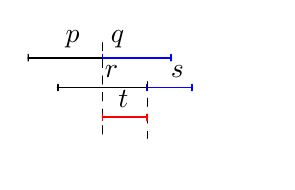
\begin{tikzpicture}[line cap=round,line join=round,>=triangle 45,x=1.0cm,y=1.0cm, scale = 0.38]
\clip(-1,-2) rectangle (7,2.5);
%\draw [->] (-1,-1 ) -- (5, -1);
%\node [right] at (4.8, -1) {\tiny time};
\draw [line width = 0.7pt] (-1,1.5) -- (1.5,1.5);
\draw [line width = 0.7pt] (-1,1.4) -- (-1,1.6);

\node [above] at (0.5,1.5) { $p$};
\draw [line width = 0.7pt, blue] (1.5,1.5) -- (3.8,1.5);
\draw [line width = 0.7pt,blue] (1.5,1.4) -- (1.5,1.6);
\draw [line width = 0.7pt,blue] (3.8,1.4) -- (3.8,1.6);

\node [above] at (2,1.5) { $q$};
\draw [black, dashed ] (1.5,2) -- (1.5,-1.2);

%-- r
\draw [line width = 0.7pt] (0,0.5) -- (3,0.5);
\draw [line width = 0.7pt] (0,0.4) -- (0,0.6);

\node [above] at (1.8,0.5) { $r$};

%--- s
\draw [line width = 0.7pt, blue] (3,0.5) -- (4.5,0.5);
\draw [line width = 0.7pt, blue] (3,0.4) -- (3,0.6);
\draw [line width = 0.7pt, blue] (4.5,0.4) -- (4.5,0.6);

\node [above] at (4,0.5) { $s$};
\draw [black, dashed ] (3,0.7) -- (3,-1.2);

%---- t
\draw [line width = 0.7pt, red] (1.5,-0.5) -- (3,-0.5);
\draw [line width = 0.7pt, red] (1.5,-0.4) -- (1.5,-0.6);
\draw [line width = 0.7pt, red] (3,-0.4) -- (3,-0.6);

\node [above] at (2.2,-0.5) { $t$};

\end{tikzpicture}\label{fig:M2c2}
} \qquad\qquad
\subfloat[$\exists t.~r||t\land t||q$: The meeting point of $r$ and $s$ precedes the meeting point of $p$ and $q$]{
\begin{tikzpicture}[line cap=round,line join=round,>=triangle 45,x=1.0cm,y=1.0cm, scale = 0.38]
\clip(-1,-2) rectangle (7,2.5);
%\draw [->] (-1,-1 ) -- (5, -1);
%\node [right] at (4.8, -1) {\tiny time};
\draw [line width = 0.7pt] (-1,1.5) -- (1.5,1.5);
\draw [line width = 0.7pt] (-1,1.4) -- (-1,1.6);

\node [above] at (0.5,1.5) { $r$};
\draw [line width = 0.7pt, blue] (1.5,1.5) -- (2,1.5);
\draw [line width = 0.7pt,blue] (1.5,1.4) -- (1.5,1.6);
\draw [line width = 0.7pt,blue] (2,1.4) -- (2,1.6);

\node [above] at (1.8,1.5) { $s$};
\draw [black, dashed ] (1.5,2) -- (1.5,-1.2);

%-- p
\draw [line width = 0.7pt] (1.9,0.5) -- (3,0.5);
\draw [line width = 0.7pt] (1.9,0.4) -- (1.9,0.6);

\node [above] at (2.5,0.5) { $p$};

%--- q
\draw [line width = 0.7pt, blue] (3,0.5) -- (4.5,0.5);
\draw [line width = 0.7pt,blue] (3,0.4) -- (3,0.6);
\draw [line width = 0.7pt,blue] (4.5,0.4) -- (4.5,0.6);

\node [above] at (4,0.5) { $q$};
\draw [black, dashed ] (3,0.7) -- (3,-1.2);

%---- t
\draw [line width = 0.7pt, red] (1.5,-0.5) -- (3,-0.5);
\draw [line width = 0.7pt, red] (1.5,-0.4) -- (1.5,-0.6);
\draw [line width = 0.7pt, red] (3,-0.4) -- (3,-0.6);

\node [above] at (2.2,-0.5) { $t$};
\end{tikzpicture}\label{fig:M2c3}
} 


\caption{The three cases of axiom (M2)}
\label{fig:M2}
\end{figure}


\section{Formalization of Time Interval Relations}
\label{sect:arel}
%Allen's time interval relations come with the operations converse, union, intersection and composition. Theory Relation.thy provides the operations that we need to use. We explain the formalization of Points are not covered by Allen's interval calculus.
%Allen's 13 relations between time intervals are shown in Fig.~\ref{fig:arels}. Hereafter, relations before, meets, overlaps, starts, finishes, during and equal are abbreviated to \texttt{b}, \texttt{m}, \texttt{ov}, \texttt{s}, \texttt{f}, \texttt{d} and \texttt{e}, respectively. 

%\subsection{ Basic Relations}

%Unions of basic relations are relations. %Let $\mathcal{R}$ be the set of the 13 relations of time intervals as follows. $$\mathcal{R} = \{e, b, b^{-1}, m, m^{-1},  ov, ov^{-1}, s, s^{-1} f, f^{-1}, d, d^{-1}\}.$$ %They establish relations between intervals of time. 
%Time interval relations describe a qualitative knowledge. When the relation between two events is completely known, then it is represented with one of the 13 time interval relations that we call \textit{basic} relations. For example, the statement  ``Tarski (T) lived after Euclid (E)."  unambiguously expresses that Euclid's life preceded Tarski's life, which can be represented (T, E) $\in$ \texttt{b}$^{-1}$ (or (E, T) $\in$ \texttt{b}). 
%
%Sometimes, the knowledge is incomplete and in that case it is represented as union of basic relations. The statement ``Hilbert (H) was born before Tarski (T)." lacks information about who died first and whether one was born after the death of the other, etc.  Nevertheless, we still can  represent these various situations as follows (H, T) $\in$ \texttt{b} $\cup$ \texttt{ov} $\cup$ \texttt{m} $\cup$ \texttt{d}$^{-1}$ $\cup$ \texttt{f}$^{-1}$, i.e.~the life of Hilbert is either before or meets or includes or finishes by the life of Tarski. We can derive new qualitative knowledge by composing relations. The relation (H, E) is the composition of relations  \texttt{b} $\cup$ \texttt{ov} $\cup$ \texttt{m} $\cup$ \texttt{d}$^{-1}$ $\cup$ \texttt{f}$^{-1}$ and \texttt{b}$^{-1}$.
%
%For simplicity, $(r_1, \ldots, r_n)$ denotes the union of basic relations $r_1, \ldots, r_n$. Thus, $x \in (r_1, \ldots, r_n)$ is equivalent to $x \in r_1 \lor \ldots \lor  x \in r_n$. Let $\alpha_1 = (r_1, \ldots, r_i)$ and $\alpha_2 = (r_1', \ldots, r_j')$, we denote by $\alpha_1 + \alpha_2$ the union of relations $r_1, \ldots, r_i, r_1', \ldots, r_j'$, i.e.~$\alpha_1 + \alpha_2 = (r_1, \ldots, r_i, r_1', \ldots, r_j')$. 
%
%\subsection{ Basic Relations}


A basic relation is a set of interval pairs  and of type {\isacharparenleft}{\isacharprime}a{\isasymtimes}{\isacharprime}a{\isacharparenright}\ set.  We extend type class \texttt{interval} with basic relations. %Let \texttt{arelations} be a type class that inherits type class interval plus additional assumptions that define the basic relations.  
\begin{isabellebody}
\isanewline
\isacommand{class}\isamarkupfalse%
\ arelations\ {\isacharequal}\ interval\ {\isacharplus}\ \isanewline
\ \isakeyword{fixes}\ \isanewline
\ \ e{\isacharcolon}{\isacharcolon}{\isachardoublequoteopen}{\isacharparenleft}{\isacharprime}a{\isasymtimes}{\isacharprime}a{\isacharparenright}\ set{\isachardoublequoteclose}\ \isakeyword{and}\isanewline
\ \ m{\isacharcolon}{\isacharcolon}{\isachardoublequoteopen}{\isacharparenleft}{\isacharprime}a{\isasymtimes}{\isacharprime}a{\isacharparenright}\ set{\isachardoublequoteclose}\ \isakeyword{and}\ \isanewline
\ \ b{\isacharcolon}{\isacharcolon}{\isachardoublequoteopen}{\isacharparenleft}{\isacharprime}a{\isasymtimes}{\isacharprime}a{\isacharparenright}\ set{\isachardoublequoteclose}\ \isakeyword{and}\isanewline
\ \ ov{\isacharcolon}{\isacharcolon}{\isachardoublequoteopen}{\isacharparenleft}{\isacharprime}a{\isasymtimes}{\isacharprime}a{\isacharparenright}\ set{\isachardoublequoteclose}\ \isakeyword{and}\isanewline
\ \ d{\isacharcolon}{\isacharcolon}{\isachardoublequoteopen}{\isacharparenleft}{\isacharprime}a{\isasymtimes}{\isacharprime}a{\isacharparenright}\ set{\isachardoublequoteclose}\ \isakeyword{and}\isanewline
\ \ s{\isacharcolon}{\isacharcolon}{\isachardoublequoteopen}{\isacharparenleft}{\isacharprime}a{\isasymtimes}{\isacharprime}a{\isacharparenright}\ set{\isachardoublequoteclose}\ \isakeyword{and}\isanewline
\ \ f{\isacharcolon}{\isacharcolon}{\isachardoublequoteopen}{\isacharparenleft}{\isacharprime}a{\isasymtimes}{\isacharprime}a{\isacharparenright}\ set{\isachardoublequoteclose}\ \ \isanewline
\isakeyword{assumes}\isanewline
\ \ e{\isacharcolon}{\isachardoublequoteopen}{\isacharparenleft}p{\isacharcomma}q{\isacharparenright}\ {\isasymin}\ e\ {\isacharequal}\ {\isacharparenleft}p\ {\isacharequal}\ q{\isacharparenright}{\isachardoublequoteclose}\ \isakeyword{and}\isanewline
\ \ m{\isacharcolon}{\isachardoublequoteopen}{\isacharparenleft}p{\isacharcomma}q{\isacharparenright}\ {\isasymin}\ m\ {\isacharequal}\ p{\isasymparallel}q{\isachardoublequoteclose}\ \isakeyword{and}\isanewline
\ \ b{\isacharcolon}{\isachardoublequoteopen}{\isacharparenleft}p{\isacharcomma}q{\isacharparenright}\ {\isasymin}\ b\ {\isacharequal}\ {\isacharparenleft}{\isasymexists}t{\isacharcolon}{\isacharcolon}{\isacharprime}a{\isachardot}\ p{\isasymparallel}t\ {\isasymand}\ t{\isasymparallel}q{\isacharparenright}{\isachardoublequoteclose}\ \isakeyword{and}\isanewline
\ \ ov{\isacharcolon}{\isachardoublequoteopen}{\isacharparenleft}p{\isacharcomma}q{\isacharparenright}\ {\isasymin}\ ov\ {\isacharequal}\ {\isacharparenleft}{\isasymexists}k\ l\ u\ v\ t{\isacharcolon}{\isacharcolon}{\isacharprime}a{\isachardot}\ {\isacharparenleft}k{\isasymparallel}p\ {\isasymand}\ p{\isasymparallel}u\ {\isasymand}\ u{\isasymparallel}v{\isacharparenright}\ {\isasymand}\   \isanewline
\ \ \ \ \ \ \ \ \ \ \ \ \ \ \ \ \ \ \ {\isacharparenleft}k{\isasymparallel}l\ {\isasymand}\ l{\isasymparallel}q\ {\isasymand}\ q{\isasymparallel}v{\isacharparenright}\ {\isasymand}\ {\isacharparenleft}l{\isasymparallel}t\ {\isasymand}\ t{\isasymparallel}u{\isacharparenright}{\isacharparenright}{\isachardoublequoteclose}\ \isakeyword{and}\isanewline
\ \ s{\isacharcolon}{\isachardoublequoteopen}{\isacharparenleft}p{\isacharcomma}q{\isacharparenright}\ {\isasymin}\ s\ {\isacharequal}\ \ {\isacharparenleft}{\isasymexists}k\ u\ v{\isacharcolon}{\isacharcolon}{\isacharprime}a{\isachardot}\ k{\isasymparallel}p\ {\isasymand}\ p{\isasymparallel}u\ {\isasymand}\ u{\isasymparallel}v\ {\isasymand}\ k{\isasymparallel}q\ {\isasymand}\ q{\isasymparallel}v{\isacharparenright}{\isachardoublequoteclose}\ \isakeyword{and}\isanewline
\ \ f{\isacharcolon}{\isachardoublequoteopen}{\isacharparenleft}p{\isacharcomma}q{\isacharparenright}\ {\isasymin}\ f\ {\isacharequal}\ {\isacharparenleft}{\isasymexists}k\ l\  u {\isacharcolon}{\isacharcolon}{\isacharprime}a{\isachardot}\ k{\isasymparallel}l\ {\isasymand}\ l{\isasymparallel}p\ {\isasymand}\ p{\isasymparallel}u\ {\isasymand}\ k{\isasymparallel}q\ {\isasymand}\ q{\isasymparallel}u{\isacharparenright}{\isachardoublequoteclose}\ \isakeyword{and}\isanewline
\ \ d{\isacharcolon}{\isachardoublequoteopen}{\isacharparenleft}p{\isacharcomma}q{\isacharparenright}\ {\isasymin}\ d\ {\isacharequal}\ {\isacharparenleft}{\isasymexists}k\ l\ u\ v{\isacharcolon}{\isacharcolon}{\isacharprime}a{\isachardot}\ k{\isasymparallel}l\ {\isasymand}\ l{\isasymparallel}p\ {\isasymand}\ p{\isasymparallel}u\ {\isasymand}u{\isasymparallel}v\ {\isasymand}\ k{\isasymparallel}q\ {\isasymand}\ q{\isasymparallel}v{\isacharparenright}{\isachardoublequoteclose}\isanewline %
%\isacommand{class}\isamarkupfalse%
%\ arelations\ {\isacharequal}\ interval\ {\isacharplus}\ \isanewline
%\ \isakeyword{fixes}\ \isanewline
%\ \ e{\isacharcolon}{\isacharcolon}{\isachardoublequoteopen}{\isacharparenleft}{\isacharprime}a{\isasymtimes}{\isacharprime}a{\isacharparenright}\ set{\isachardoublequoteclose}\ \isakeyword{and}\isanewline
%\ \ m{\isacharcolon}{\isacharcolon}{\isachardoublequoteopen}{\isacharparenleft}{\isacharprime}a{\isasymtimes}{\isacharprime}a{\isacharparenright}\ set{\isachardoublequoteclose}\ \isakeyword{and}\ \isanewline
%\ \ b{\isacharcolon}{\isacharcolon}{\isachardoublequoteopen}{\isacharparenleft}{\isacharprime}a{\isasymtimes}{\isacharprime}a{\isacharparenright}\ set{\isachardoublequoteclose}\ \isakeyword{and}\isanewline
%\ \ ov{\isacharcolon}{\isacharcolon}{\isachardoublequoteopen}{\isacharparenleft}{\isacharprime}a{\isasymtimes}{\isacharprime}a{\isacharparenright}\ set{\isachardoublequoteclose}\ \isakeyword{and}\isanewline
%\ \ d{\isacharcolon}{\isacharcolon}{\isachardoublequoteopen}{\isacharparenleft}{\isacharprime}a{\isasymtimes}{\isacharprime}a{\isacharparenright}\ set{\isachardoublequoteclose}\ \isakeyword{and}\isanewline
%\ \ s{\isacharcolon}{\isacharcolon}{\isachardoublequoteopen}{\isacharparenleft}{\isacharprime}a{\isasymtimes}{\isacharprime}a{\isacharparenright}\ set{\isachardoublequoteclose}\ \isakeyword{and}\isanewline
%\ \ f{\isacharcolon}{\isacharcolon}{\isachardoublequoteopen}{\isacharparenleft}{\isacharprime}a{\isasymtimes}{\isacharprime}a{\isacharparenright}\ set{\isachardoublequoteclose}\ \ \isanewline
%\isakeyword{assumes}
%\ \ \isanewline
%\ \  e{\isacharcolon}{\isachardoublequoteopen}{\isacharparenleft}p{\isacharcomma}q{\isacharparenright}\ {\isasymin}\ e\ {\isacharequal}\ {\isacharparenleft}\ p\ {\isacharequal}\ q{\isacharparenright}{\isachardoublequoteclose}\ \isakeyword{and}\isanewline
%\ \ m{\isacharcolon}{\isachardoublequoteopen}{\isacharparenleft}p{\isacharcomma}q{\isacharparenright}\ {\isasymin}\ m\ {\isacharequal}\ p{\isasymparallel}q{\isachardoublequoteclose}\ \isakeyword{and}\isanewline
%\ \ b{\isacharcolon}{\isachardoublequoteopen} {\isacharparenleft}p{\isacharcomma}q{\isacharparenright}\ {\isasymin}\ b\ {\isacharequal}\  {\isacharparenleft}{\isasymexists}r{\isacharcolon}{\isacharcolon}{\isacharprime}a{\isachardot}\ p{\isasymparallel}r\ {\isasymand}\ r{\isasymparallel}q{\isacharparenright}{\isachardoublequoteclose}\ \isakeyword{and}\isanewline
%\ \ ov{\isacharcolon}{\isachardoublequoteopen}{\isacharparenleft}p{\isacharcomma}q{\isacharparenright}\ {\isasymin}\ ov\ {\isacharequal}\ \ {\isacharparenleft}{\isasymexists}r\ s\ t\ u\ v{\isacharcolon}{\isacharcolon}{\isacharprime}a{\isachardot}\ \isanewline
%\ \ \ \ \ \ \ \ \ \ \ \ \ \ \ \ \ \  \ \ \ {\isacharparenleft}r{\isasymparallel}p\ {\isasymand}\ p{\isasymparallel}u\ {\isasymand}\ u{\isasymparallel}v{\isacharparenright}\ {\isasymand} {\isacharparenleft}r{\isasymparallel}s\ {\isasymand}\ s{\isasymparallel}q\ {\isasymand}\ q{\isasymparallel}v{\isacharparenright}\ {\isasymand}\isanewline \ \ \ \ \ \ \ \ \ \ \ \ \ \ \ \ \ \  \ \ \  {\isacharparenleft}s{\isasymparallel}t\ {\isasymand}\ t{\isasymparallel}u{\isacharparenright}{\isacharparenright}{\isachardoublequoteclose}\ \isakeyword{and}\isanewline
%\ \ s{\isacharcolon}{\isachardoublequoteopen}{\isacharparenleft}p{\isacharcomma}q{\isacharparenright}\ {\isasymin}\ s\ {\isacharequal}\ \ {\isacharparenleft}{\isasymexists}t\ u\ v{\isacharcolon}{\isacharcolon}{\isacharprime}a{\isachardot}\ t{\isasymparallel}p\ {\isasymand}\ p{\isasymparallel}u\ {\isasymand}\ u{\isasymparallel}v\ {\isasymand}\ t{\isasymparallel}q\ {\isasymand}\ q{\isasymparallel}v{\isacharparenright}{\isachardoublequoteclose}\ \isakeyword{and}\isanewline
%\ \ f{\isacharcolon}{\isachardoublequoteopen}{\isacharparenleft}p{\isacharcomma}q{\isacharparenright}\ {\isasymin}\ f\ {\isacharequal}\ {\isacharparenleft}{\isasymexists}t\ s\ u\ {\isacharcolon}{\isacharcolon}{\isacharprime}a{\isachardot}\ t{\isasymparallel}s\ {\isasymand}\ s{\isasymparallel}p\ {\isasymand}\ p{\isasymparallel}u\ {\isasymand}\ t{\isasymparallel}q\ {\isasymand}\ q{\isasymparallel}u{\isacharparenright}{\isachardoublequoteclose}\ \isakeyword{and}\isanewline
%\ \ d{\isacharcolon}{\isachardoublequoteopen}{\isacharparenleft}p{\isacharcomma}q{\isacharparenright}\ {\isasymin}\ d\ {\isacharequal}\ {\isacharparenleft}{\isasymexists}t\ s\ u\ v{\isacharcolon}{\isacharcolon}{\isacharprime}a{\isachardot}\ t{\isasymparallel}s\ {\isasymand}\ s{\isasymparallel}p\ {\isasymand}\ p{\isasymparallel}u\ {\isasymand}u{\isasymparallel}v\ {\isasymand}\ t{\isasymparallel}q\ {\isasymand}\ q{\isasymparallel}v{\isacharparenright}{\isachardoublequoteclose}\isanewline 
%\isakeyword{and}\isanewline
%\ \ nonempty{\isacharcolon}{\isachardoublequoteopen}{\isasymforall}r\ {\isasymin}\ \ {\isacharbraceleft}e{\isacharcomma}m{\isacharcomma}b{\isacharcomma}ov{\isacharcomma}s{\isacharcomma}f{\isacharcomma}d{\isacharcomma}e{\isacharcircum}{\isacharminus}{\isadigit{1}}{\isacharcomma}m{\isacharcircum}{\isacharminus}{\isadigit{1}}{\isacharcomma}b{\isacharcircum}{\isacharminus}{\isadigit{1}}{\isacharcomma}ov{\isacharcircum}{\isacharminus}{\isadigit{1}}{\isacharcomma}s{\isacharcircum}{\isacharminus}{\isadigit{1}}{\isacharcomma}f{\isacharcircum}{\isacharminus}{\isadigit{1}}{\isacharcomma}d{\isacharcircum}{\isacharminus}{\isadigit{1}}{\isacharbraceright}{\isachardot}\ {\isasymexists}p\ q{\isacharcolon}{\isacharcolon}{\isacharprime}a{\isachardot}\ {\isacharparenleft}p{\isacharcomma}q{\isacharparenright}\ {\isasymin}\ r\ {\isachardoublequoteclose}\ \isakeyword{and}\isanewline
%\ \isanewline
%\ \ JE{\isacharcolon}{\isachardoublequoteopen}e\ {\isasymunion}\ m\ {\isasymunion}\ m{\isacharcircum}{\isacharminus}{\isadigit{1}}\ {\isasymunion}\ b\ {\isasymunion}\ b{\isacharcircum}{\isacharminus}{\isadigit{1}}\ {\isasymunion}\ ov\ {\isasymunion}\ ov{\isacharcircum}{\isacharminus}{\isadigit{1}}\ {\isasymunion}\ s\ {\isasymunion}\ s{\isacharcircum}{\isacharminus}{\isadigit{1}}\ {\isasymunion}\ f\ {\isasymunion}\ f{\isacharcircum}{\isacharminus}{\isadigit{1}}\ {\isasymunion}\ d\ {\isasymunion}\ d{\isacharcircum}{\isacharminus}{\isadigit{1}}\ {\isacharequal}\ {\isacharbraceleft}{\isacharparenleft}p{\isacharcomma}q{\isacharparenright}\ {\isacharbar}\ p\ q{\isacharcolon}{\isacharcolon}{\isacharprime}a{\isachardot}\ \ {\isasymI}\ p\ {\isasymand}\ {\isasymI}\ q{\isacharbraceright}{\isachardoublequoteclose}\ \isanewline
\end{isabellebody}

%It was shown that Allen's calculus is a a relation algebra~\cite{Dylla:2013}. \textcolor{red}{$\leftarrow$ How this relevant to this formalization?}. 
% Basic relations are defined using relations ``$||$" and ``=" between intervals. 

In the assumptions of class \texttt{arelations}, each basic time interval relation is rewritten as a first order formula in a prenex normal form, i.e.~a conjunction of atomic formulas $x || y$ and $x  = y$. 
Relations \texttt{e}, \texttt{m} and \texttt{b}  are self-explanatory. Rewriting rules of the remaining relations are illustrated in Fig.~\ref{fig:arelations}. % how they are defined with meets and equal.  


We call literal the atomic formula of the form $x||y$ and $x=y$. % in the prenex normal form formulas that describe basic relations. %The rules e, m, b, ov, s, f and d are conjunctions of literals. In a relation membership $(p,q) \in r$, rule r gives rise to a set of literals. 
We denote by $L_r(p,q)$ the set of literals generated by the relation membership $(p,q) \in r$. Among the literals in $L_r(p,q)$, there are constraints on the starting points and the ending points of intervals $p$ and $q$. For instance,  $(p,q) \in$ \texttt{ov} gives rise to the eight literals \{$k||p$, $p||u$, $u||v$, $k||l$, $l||q$, $q||v$, $l||t$ , $t||u$\} = $L_{\texttt{ov}}(p,q)$. Literals $k||p$ and $l||q$ are constraints on the starting points of $p$ and $q$. Literals $p||u$ and $q||v$ are constraints on the ending points of $p$ and $q$.  


%We call basic relations the 13 relations in Fig.~\ref{fig:arels}. 
%
%There are $2^{13}$ time interval relations to express the arrangements between events. For simplicity, $(r_1, \ldots, r_n)$ denotes the union of basic relations $r_1, \ldots, r_n$. Thus, $x \in (r_1, \ldots, r_n)$ is equivalent to $x \in r_1 \lor \ldots \lor  x \in r_n$. Let $\alpha_1 = (r_1, \ldots, r_i)$ and $\alpha_2 = (r_1', \ldots, r_j')$, we denote by $\alpha_1 + \alpha_2$ the union of relations $r_1, \ldots, r_i, r_1', \ldots, r_j'$, i.e.~$\alpha_1 + \alpha_2 = (r_1, \ldots, r_i, r_1', \ldots, r_j')$. %Moreover, the inverse of a union of relations is the union of the inverse relations. In other words, we have $(r_1, \ldots, r_n)^{-1} = (r_1^{-1}, \ldots, r_n^{-1})$.



\begin{figure}
\centering
\subfloat[$(p,q)\in$ \texttt{ov}]
{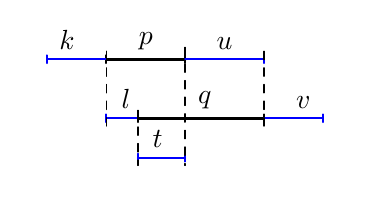
\begin{tikzpicture}[line cap=round,line join=round,>=triangle 45,x=1.0cm,y=1.0cm, scale = 0.5]
\clip(-1,-2) rectangle (7,1.8);
\node [above] at (2,1) { $p$};
\draw [line width = 1.2pt] (1,1) -- (3,1);
\draw [line width = 0.7pt] (1,1.1) -- (1,0.9);
\draw [line width = 0.7pt] (3,1.1) -- (3,0.9);

\node [above] at (3.5,-0.5) { $q$};
\draw [line width = 1.2pt] (1.8,-0.5) -- (5,-0.5);
\draw [line width = 0.7pt] (1.8,-0.4) -- (1.8,-0.6);
\draw [line width = 0.7pt] (5,-0.4) -- (5,-0.6);

%% r
\node [above] at (0,1) {$k$};
\draw [line width = 0.7pt, blue] (-0.5,1) -- (1,1);
\draw [line width = 0.7pt, blue] (-0.5,1.1) -- (-0.5,0.9);
%\draw [line width = 0.7pt, blue] (1,1.1) -- (1,0.9);
%% u
\node [above] at (4,1) {$u$};
\draw [line width = 0.7pt, blue] (3,1) -- (5,1);
%\draw [line width = 0.7pt, blue] (3,1.1) -- (3,0.9);
\draw [line width = 0.7pt, blue] (5,1.1) -- (5,0.9);
%% s
\node [above] at (1.5,-0.5) {$l$};
\draw [line width = 0.7pt, blue] (1,-0.5) -- (1.8,-0.5);
\draw [line width = 0.7pt, blue] (1,-0.4) -- (1,-0.6);
%% v
\node [above] at (6,-0.5) {$v$};
\draw [line width = 0.7pt, blue] (5,-0.5) -- (6.5,-0.5);
\draw [line width = 0.7pt, blue] (6.5,-0.4) -- (6.5,-0.6);
%% t
\node [above] at (2.3,-1.5) { $t$};
\draw [line width = 0.7pt,blue] (1.8,-1.5) -- (3,-1.5);
\draw [line width = 0.7pt,blue] (1.8,-1.4) -- (1.8,-1.6);
\draw [line width = 0.7pt,blue] (3,-1.4) -- (3,-1.6);

%% dashed
\draw [line width=0.5pt, dashed] (1,1.2) -- (1,-0.7);
\draw [line width=0.5pt, dashed] (5,1.2) -- (5,-0.7);
\draw [line width=0.5pt, dashed] (1.8,-0.3) -- (1.8,-1.7);
\draw [line width=0.5pt, dashed] (3,1.3) -- (3,-1.7);
\end{tikzpicture}\label{fig:ov}
} \quad
\subfloat[$(p,q)\in$ \texttt{s}]
{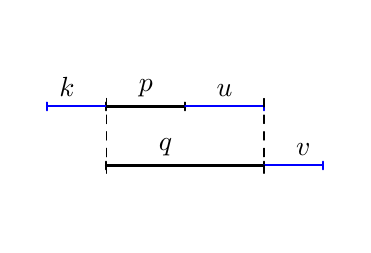
\begin{tikzpicture}[line cap=round,line join=round,>=triangle 45,x=1.0cm,y=1.0cm, scale = 0.5]
\clip(-1,-2) rectangle (7,3);
\node [above] at (2,1) { $p$};
\draw [line width = 1.2pt] (1,1) -- (3,1);
\draw [line width = 0.7pt] (1,1.1) -- (1,0.9);
\draw [line width = 0.7pt] (3,1.1) -- (3,0.9);

\node [above] at (2.5,-0.5) { $q$};
\draw [line width = 1.2pt] (1,-0.5) -- (5,-0.5);
\draw [line width = 0.7pt] (1,-0.4) -- (1,-0.6);
\draw [line width = 0.7pt] (5,-0.4) -- (5,-0.6);

%%t
\node [above] at (0,1) {$k$};
\draw [line width = 0.7pt, blue] (-0.5,1) -- (1,1);
\draw [line width = 0.7pt, blue] (-0.5,1.1) -- (-0.5,0.9);

%% u
\node [above] at (4,1) {$u$};
\draw [line width = 0.7pt, blue] (3,1) -- (5,1);
%\draw [line width = 0.7pt, blue] (3,1.1) -- (3,0.9);
\draw [line width = 0.7pt, blue] (5,1.1) -- (5,0.9);

%% v
\node [above] at (6,-0.5) {$v$};
\draw [line width = 0.7pt, blue] (5,-0.5) -- (6.5,-0.5);
\draw [line width = 0.7pt, blue] (6.5,-0.4) -- (6.5,-0.6);

%% dashed
\draw [line width=0.5pt, dashed] (1,1.2) -- (1,-0.7);
\draw [line width=0.5pt, dashed] (5,1.2) -- (5,-0.7);

\end{tikzpicture}\label{fig:s}}\qquad\qquad
\subfloat[$(p,q)\in$ \texttt{f}]
{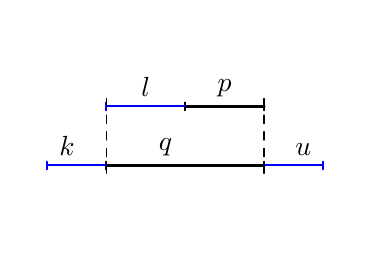
\begin{tikzpicture}[line cap=round,line join=round,>=triangle 45,x=1.0cm,y=1.0cm, scale = 0.5]
\clip(-1,-2) rectangle (7,3);
\node [above] at (4,1) { $p$};
\draw [line width = 1.2pt] (3,1) -- (5,1);
\draw [line width = 0.7pt] (3,1.1) -- (3,0.9);
\draw [line width = 0.7pt] (5,1.1) -- (5,0.9);

\node [above] at (2.5,-0.5) { $q$};
\draw [line width = 1.2pt] (1,-0.5) -- (5,-0.5);
\draw [line width = 0.7pt] (1,-0.4) -- (1,-0.6);
\draw [line width = 0.7pt] (5,-0.4) -- (5,-0.6);

%t
\node [above] at (0,-0.5) {$k$};
\draw [line width = 0.7pt, blue] (-0.5,-0.5) -- (1,-0.5);
\draw [line width = 0.7pt, blue] (-0.5,-0.4) -- (-0.5,-0.6);

%% s
\node [above] at (2,1) {$l$};
\draw [line width = 0.7pt, blue] (1,1) -- (3,1);
\draw [line width = 0.7pt, blue] (1,1.1) -- (1,0.9);
%% u
\node [above] at (6,-0.5) {$u$};
\draw [line width = 0.7pt, blue] (5,-0.5) -- (6.5,-0.5);
\draw [line width = 0.7pt, blue] (6.5,-0.4) -- (6.5,-0.6);
%% dashed
\draw [line width=0.5pt, dashed] (1,1.2) -- (1,-0.7);
\draw [line width=0.5pt, dashed] (5,1.2) -- (5,-0.7);

\end{tikzpicture}\label{fig:f}}\qquad\qquad
\subfloat[$(p,q)\in$ \texttt{d}]
{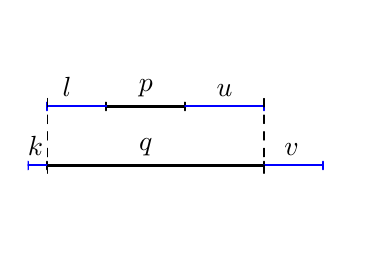
\begin{tikzpicture}[line cap=round,line join=round,>=triangle 45,x=1.0cm,y=1.0cm, scale = 0.5]
\clip(-1,-2) rectangle (7,3);

\node [above] at (2,1) { $p$};
\draw [line width = 1.2pt] (1,1) -- (3,1);
\draw [line width = 0.7pt] (1,1.1) -- (1,0.9);
\draw [line width = 0.7pt] (3,1.1) -- (3,0.9);

\node [above] at (2,-0.5) { $q$};
\draw [line width = 1.2pt] (-0.5,-0.5) -- (5,-0.5);
\draw [line width = 0.7pt] (-0.5,-0.4) -- (-0.5,-0.6);
\draw [line width = 0.7pt] (5,-0.4) -- (5,-0.6);

%% t
\node [above] at (-0.8,-0.5) {$k$};
\draw [line width = 0.7pt, blue] (-1,-0.5) -- (-0.5,-0.5);
\draw [line width = 0.7pt, blue] (-1,-0.4) -- (-1,-0.6);
%% s
\node [above] at (0,1) {$l$};
\draw [line width = 0.7pt, blue] (-0.5,1) -- (1,1);
\draw [line width = 0.7pt, blue] (-0.5,1.1) -- (-0.5,0.9);

%% u
\node [above] at (4,1) {$u$};
\draw [line width = 0.7pt, blue] (3,1) -- (5,1);
\draw [line width = 0.7pt, blue] (5,1.1) -- (5,0.9);

%% u
\node [above] at (5.7,-0.5) {$v$};
\draw [line width = 0.7pt, blue] (5,-0.5) -- (6.5,-0.5);
\draw [line width = 0.7pt, blue] (6.5,-0.4) -- (6.5,-0.6);

%% dashed
\draw [line width=0.5pt, dashed] (-0.5,1.2) -- (-0.5,-0.7);
\draw [line width=0.5pt, dashed] (5,1.2) -- (5,-0.7);

\end{tikzpicture}\label{fig:d}
} 
\caption{Relations \texttt{ov}, \texttt{s}, \texttt{f} and \texttt{d} defined as conjunctions of literals of the form $x||y$, where $x$ and $y$ are time intervals}
\label{fig:arelations}
\end{figure}


%There are $2^{13}$ time interval relations to express the arrangements between events.  
%In this formalization of Allen's calculus, we use the operations union, inverse, intersection and composition. 

%For simplicity, $(r_1, \ldots, r_n)$ denotes the union of basic relations $r_1, \ldots, r_n$. Thus, $x \in (r_1, \ldots, r_n)$ is equivalent to $x \in r_1 \lor \ldots \lor  x \in r_n$. Let $\alpha_1 = (r_1, \ldots, r_i)$ and $\alpha_2 = (r_1', \ldots, r_j')$, we denote by $\alpha_1 + \alpha_2$ the union of relations $r_1, \ldots, r_i, r_1', \ldots, r_j'$, i.e.~$\alpha_1 + \alpha_2 = (r_1, \ldots, r_i, r_1', \ldots, r_j')$.  The composition $\alpha_1\; \circ \; \alpha_2$ is the relation $(r_1 \circ r_1', r_1 \circ r_2', \ldots, r_1 \circ r_n', \ldots, r_n \circ r_1', r_n \circ r_2',\ldots, r_n \circ r_n')$.

%We also need to use inverse and intersection. The inverse of a union of relations is the union of the inverse relations. In other words, we have $(r_1, \ldots, r_n)^{-1} = (r_1^{-1}, \ldots, r_n^{-1})$. Similarly, the intersection of a union is the union of intersections. %, i.e.~$\alpha_1 \cap \alpha_2 = (r_1 \cap r_1', r_1 \cap r_2', \ldots, r_1 \cap r_n', \ldots, r_n \cap r_1', r_n \cap r_2',\ldots, r_n \cap r_n')$.

%Theory Relation.thy provides the operations that we need.


%Expressiveness
\section{JEPD Property}
\label{sect:jepd}
In qualitative reasoning, representations of events or objects in the space are based on a set of relations that are jointly exhaustive (JE) and pairwise disjoint (PD). JE property ensures the expressiveness of the relations.  
%The 13 basic relations constitute a partition of the set of all the possible relationships between two intervals. 
In other words, for any two intervals, there exists a relation that holds between these two intervals. The 13 time interval relations, therefore, constitute a partition of the set of interval pairs. %\textcolor{red}%{ i.e.~the set of well defined intervals $\{(p,q)\; |\;\forall p\;q:{\isacharprime} a.\;\mathcal{I}\;p\;\land\mathcal{I}\;q\}$. The $\mathcal{I}$ predicate is to ensure that intervals are well defined. For instance, the starting point of a real interval is strictly less than the ending point. The well defined predicate is introduced by type class interval?}

The unicity of a relation between two arbitrary intervals is allowed by the PD property.  Therefore, the 13 relations enable us to express precise information between any two temporal intervals and avoid redundancy. 

%Let $\delta$ be the set of the 13 relations of time intervals as follows. $$\delta = (b,m,ov, s, d, f, e, f^{-1}, d^{-1}, s^{-1}, ov^{-1}, m^{-1}, b^{-1}).$$ Next, we explain the proofs of JEPD property.
%\vskip 1em
\subsubsection{PD property.} 
For any two different basic relations $r_1$ and $r_2$, we show that $r_1\; \cap\; r_2 = \{\}$. The proof is performed by contradiction. From $(p,q) \in r_1$ and $(p,q) \in r_2$, we deduce literals that refute the non-transitivity property of ``$||$", i.e. property \texttt{meets\_atrans}. %deducing %\footnote{\textcolor{red}{This requires checking disequalities of relations.}} %, for any $r_1, r_2 \in \mathcal{R}$. 
%We prove all PD lemmas ($\sum_{1}^{12} (13 - i) = 78$ in total). 
%We explain two proofs. 
%The following lemma \texttt{m} $\cap$ \texttt{b} $=\{\}$ is immediately proved from the non-transitivity of ``$||$". 
\begin{isabellebody}
\isanewline
\isacommand{lemma}\isamarkupfalse%
\ {\isachardoublequoteopen}m\ {\isasyminter}\ b\ {\isacharequal}\ {\isacharbraceleft}{\isacharbraceright}{\isachardoublequoteclose}\isanewline
%
%\isadelimproof
%
%\endisadelimproof
%
%\isatagproof
\isacommand{using}\isamarkupfalse%
\ m\ b\ \isacommand{apply}\isamarkupfalse%
\ auto\isanewline
\isacommand{using}\isamarkupfalse%
\ meets\_atrans\ \isacommand{by}\isamarkupfalse%
\ blast%
\isanewline
%\endisatagproof
{\isafoldproof}%
%
%\isadelimproof
\end{isabellebody}

%Lemma \texttt{elimmeets1} states that two intervals cannot, at the same time, meet and be separated.
%\begin{isabellebody}
%\isanewline
%\isacommand{lemma}\isamarkupfalse%
%\ elimmeets1{\isacharcolon}\isanewline
%\isakeyword{shows}\  {\isachardoublequoteopen}p\ {\isasymparallel}\ q\ {\isasymand}\ {\isacharparenleft}{\isasymexists}t{\isachardot}\ p\ {\isasymparallel}\ t\ {\isasymand}\ t\ {\isasymparallel}\ q{\isacharparenright}\ %{\isasymand}\ {\isacharparenleft}{\isasymexists}t{\isachardot}\ r\ {\isasymparallel}\ t\ {\isasymand}\ t\ {\isasymparallel}\ q{\isacharparenright}{\isacharparenright}\
% {\isacharequal}\ False{\isachardoublequoteclose}\isanewline
%\end{isabellebody}
% The first line ``\isacommand{using}\isamarkupfalse%
%\ m\ b\ \isacommand{apply} \ auto" simplify the goal, uses proof by contradiction, i.e. gives rise to $\bigwedge x \;y. \;(x, y) \in m \Longrightarrow (x, y) \in b \Longrightarrow False$, then rewrite relations m and b using suitable rules from type class \texttt{arelations}.  Relation b generates the literals $x||r$ and $r||y$ that give $\neg x||y$ when applying atransitivity of ``$||$", which results into contradiction with the literal ``$x||y$" from relation m. Line ``\isacommand{using}\isamarkupfalse%
%\ meets\_atrans\ \isacommand{by}\isamarkupfalse%
%\ blast" thus terminates the proof.
%\textcolor{red}{revise the above paragraph. Also, the subgoal should be written in  Isabelle/HOL meta logic.}

Relations $r_1$ and $r_2$ sometimes generate literals from which we cannot immediately deduce the contradiction. Therefore, we use the axiomatic system defined in Sect.~\ref{sect:axioms} to deduce new ``$||$" relations and obtain new intervals. The tactics \texttt{metis} and \texttt{meson}  finish the proof successfully. %, such is the case for the following lemma. 
\begin{isabellebody}
\isanewline
\isacommand{lemma}\isamarkupfalse%
 \ {\isachardoublequoteopen}s\ {\isasyminter}\ d\ {\isacharequal}\ {\isacharbraceleft}{\isacharbraceright}{\isachardoublequoteclose}\ \isanewline
%
%\isadelimproof
%%
%\endisadelimproof
%
%\isatagproof
\isacommand{apply}\isamarkupfalse%
\ \isacommand{using}\isamarkupfalse%
\ s\ d\ \isacommand{apply}\isamarkupfalse%
\ auto\isanewline
\isacommand{by}\isamarkupfalse%
\ {\isacharparenleft}meson\ M{\isadigit{1}}\ meets{\isacharunderscore}atrans{\isacharparenright}%
%\endisatagproof
{\isafoldproof}%
%
%\isadelimproof
\isanewline
\end{isabellebody}

%The above proof proceeds by contradiction. The relation s gives rise to five intervals $p, q, t, u,$ and $v$. We have $(p,q)\in s$ and $t||p$, $p||u$, $t||q$, $u||v$ and $q||v$.  From $(p,q) \in \texttt{d}$, we obtain $t'||s'$, $s'||p$, $p||u'$, $u'||v'$, $t'||q$ and $q||v'$.  In the second line of the proof, we apply Isabelle/HOL tableau method \texttt{meson}. It uses axiom (M1) to deduce a new \texttt{meets} relation, namely $t||p\land t||q\land t'||q \Longrightarrow t'||p$. Or, the atransitivity property says $t`||s`\land s'||p \Longrightarrow \neg\; t'||p$, hence it is a contradiction.

% $\sum_{1}^{12} (13 - i) = 78$
%\vskip 1em
\subsubsection{JE property.} 
Let $\delta$ be the relation that is  the union of all basic relations. $$\delta = (\texttt{b},\texttt{m},\texttt{ov}, \texttt{s}, \texttt{d}, \texttt{f}, \texttt{e}, \texttt{f}^{-1}, \texttt{d}^{-1}, \texttt{s}^{-1}, \texttt{ov}^{-1}, \texttt{m}^{-1}, \texttt{b}^{-1}).$$ 
JE property means that for any two intervals $x$ and $y$, the expression $(x, y) \in \delta$ always holds. We do not explain the proof as it is similar to the proof of $\delta$-composition in Sect.~\ref{sect:gammadelta}.


%This to ensure the expressiveness and avoid redundancy in the information that is being represented. Similarly, the 13 relations of time intervals satisfy these two properties. We show that $r_1 \cap r_2 = \{\}$ for any $r_1, r_2 \in \{e, b, b^{-1}, m, m^{-1},  ov, ov^{-1}, s, s^{-1} f, f^{-1}, d, d^{-1}\}$.  The 13 pairwise disjoint relations enable us to express ``precise" information between temporal intervals. In addition, we can introduce the possibility of representing certain vague information: the fact that x and y are disjoint, for example, which is the disjunction of x $b$ y and x $b^{-1}$ y, can be written as x {$b$, $b^{-1}$} y, by introducing sets of basic relations which are interpreted in a disjunctive manner: $(x,y) \in R$, where $R$ is a set of basic relations, signifies that for some basic relation $r \in R$, we have $(x,y) \in r$.
%
%An important property of the 13 basic relations is that they constitute a partition of the set of all the possible relationships between two intervals. In less mathematical terms, this means that, given two intervals, there exists exactly one basic relation that holds between these two intervals. 
\section{Compositions of Time Interval Relations}
\label{sect:comp}
%\subsection{Lattice of Basic Relations}
\subsection{Composition Table}
The compositions of time interval relations were first computed by Allen~\cite{Allen:1985}. We arrange the result of the compositions in Table~\ref{table1}. We read the table as follows. Let $r_1$ and $r_2$ be two of the relations given in the first column and the first row, respectively. An entry in the table is a relation that contains the composition $r_1\circ r_2$. For instance, according to the table, the composition \texttt{s} $\circ$ \texttt{m}  is a subset of relation \texttt{b}. We write \texttt{s} $\circ$ \texttt{m} $\subseteq$ \texttt{b}. Some compositions give rise to union of basic relations, e.g.~\texttt{b} $\circ$ \texttt{d}. We call them relations $\alpha$, $\beta$, $\gamma$ and $\delta$ and define them as follows.
\begin{align*}
& \alpha_1 = (\texttt{ov}, \texttt{s}, \texttt{d}) \\ %\text{ and }{\alpha_1}^{-1} = (ov^{-1}, s^{-1}, d^{-1}) \\
& \alpha_2 = (\texttt{ov}, \texttt{f}^{-1}, \texttt{d}^{-1}) \\ %\text{ and } {\alpha_2}^{-1} = (ov^{-1}, f, d)\\
& \alpha_3 = (\texttt{b}, \texttt{m}, \texttt{ov}) \\ %\text{ and } {\alpha_3}^{-1} = (b^{-1}, m^{-1}, ov^{-1})\\
&\alpha_4 = (\texttt{f}^{-1}, \texttt{e}, \texttt{f})\\
& \alpha_5 =  (\texttt{s}, \texttt{e}, \texttt{s}^{-1})\\
& \beta_1 = (\texttt{b}, \texttt{m}, \texttt{ov}, \texttt{s}, \texttt{d}) \\ %\text{ and } {\beta_1}^{-1} = (b^{-1}, m^{-1}, ov^{-1}, s^{-1}, d^{-1})\\  
& \beta_2 = (\texttt{b}, \texttt{m}, \texttt{ov}, \texttt{f}^{-1}, \texttt{d}^{-1})\\ 
& \gamma = (\texttt{ov}, \texttt{s}, \texttt{d}, \texttt{f}, \texttt{e}, \texttt{f}^{-1}, \texttt{d}^{-1}, \texttt{s}^{-1}, \texttt{ov}^{-1})\\
& \delta = (\texttt{b},\texttt{m},\texttt{ov}, \texttt{s}, \texttt{d}, \texttt{f}, \texttt{e}, \texttt{f}^{-1}, \texttt{d}^{-1}, \texttt{s}^{-1}, \texttt{ov}^{-1}, \texttt{m}^{-1}, \texttt{b}^{-1})
\end{align*}

Their inverses are deduced from the fact that the inverse of a union of relations is a union of inverse relations. %, i.e. $(r_1, \ldots, r_n)^{-1} = (r_1^{-1}, \ldots, r_n^{-1})$. 
%We thus have the following. 
\begin{align*}
& {\alpha_1}^{-1} = (\texttt{ov}^{-1}, \texttt{s}^{-1}, \texttt{d}^{-1}) \\
& {\alpha_2}^{-1} = (\texttt{ov}^{-1}, \texttt{f}, \texttt{d})\\
& {\alpha_3}^{-1} = (\texttt{b}^{-1}, \texttt{m}^{-1}, \texttt{ov}^{-1})\\
& {\alpha_4}^{-1} = (\texttt{f}^{-1}, \texttt{e}, \texttt{f})\\
&  {\alpha_5}^{-1} = (\texttt{s}, \texttt{e}, \texttt{s}^{-1})\\
&  {\beta_1}^{-1} = (\texttt{b}^{-1}, \texttt{m}^{-1}, \texttt{ov}^{-1}, \texttt{s}^{-1}, \texttt{d}^{-1})\\  
& {\beta_2}^{-1} = (\texttt{b}^{-1}, \texttt{m}^{-1}, \texttt{ov}^{-1}, \texttt{f}, \texttt{d})\\ 
& {\gamma}^{-1} = (\texttt{ov}, \texttt{s}, \texttt{d}, \texttt{f}, \texttt{e}, \texttt{f}^{-1}, \texttt{d}^{-1}, \texttt{s}^{-1}, \texttt{ov}^{-1})\\
& {\delta}^{-1} = (\texttt{b},\texttt{m},\texttt{ov}, \texttt{s}, \texttt{d}, \texttt{f}, \texttt{e}, \texttt{f}^{-1}, \texttt{d}^{-1}, \texttt{s}^{-1}, \texttt{ov}^{-1}, \texttt{m}^{-1}, \texttt{b}^{-1})
\end{align*}

The Table \ref{table1} is symmetric w.r.t.~the diagonal white cells. The relations in yellow cells  are inverse of the relations in blue cells. For instance, referring to the table, we have $\texttt{s}\; \circ \;\texttt{d}^{-1} \subseteq \beta_2$. By symmetry w.r.t.~the diagonal, we reach the yellow cell that corresponds to $\texttt{d}\; \circ\; \texttt{s}^{-1} = (\texttt{s}\; \circ \texttt{d}^{-1})^{-1} \subseteq {\beta_2}^{-1}$. Relations \texttt{e}, $\alpha_4$, $\alpha_5$, $\gamma$ and $\delta$ are closed under inversion and they appear only in the diagonal white cells. What we need to prove is the compositions that correspond to blue and white cells, the proofs of compositions given by yellow cells are then deduced immediately. %To that end, we first introduce the lattice representation of time interval basic relations

 %Relations  $\alpha_{1\leq i \leq 5}$ and $\beta_{1\leq i\leq 2}$ are unions of 3 and 5 relations, respectively. Note that $\alpha$ and $\beta$ relations are path-connected in the lattice of basic relations. Relation $\gamma$ is the union of the five relations e, s, d, f, ov and their inverse relations. Relation $\delta$ is simply the set $\mathcal{R}$ of all the 13 relations. 

%A nice representation of the basic relations is the lattice representation~\cite{Lizgot:1992} depicted in Fig.~\ref{fig:lattice}. The relations $\alpha$, $\beta$, $\gamma$ and $\delta$ are path-connected where their basic relations are ordered.  The structure of the lattice is central to the design of the proof of the composition table which we discuss later in Sect.~\ref{sect:proof}. 
%The relations in 1st column and row are arranged is such a way the entries are symmetric with respect to the diagonal. The symmetry is due to the equality $r_1 \circ \;r_2\;=\;r_2^{-1}\circ\; r_1^{-1}$. 
%What we want to prove in Isabelle/HOL is that the entries in Table~\ref{table1} are correct. We prove lemmas of the form {$r_1 \circ \;r_2 \subseteq R$}, where $R$ is a basic relation or any of the relations $\alpha_{1\leq i \leq 5}, \beta_{1\leq i \leq 2}, \gamma$ and $\delta$. 

%The proof boils down to finding three intervals $a,\; b$ and $c$ such that $(a,b) \in r_1 \land (b,c) \in r_2 \land (a,c) \in \theta$, for any basic relation $\theta$ from R.
%%are manually computed are of the form 
%\begin{itemize}
%\item[(i)] The composition table is correct: the entries $r_1 \circ r_2 $ given in Table~\ref{table1} are correct.
%\item[(ii)] The composition table is minimal: the relation \textcolor{red}{R ${\supseteq}$ $r_1 \circ \;r_2 $} is minimal, where R is a basic relation $r$ or any of the relations $\alpha_{1\leq i \leq 5}, \beta_{1\leq i \leq 2}, \gamma$ and $\delta$. In other words, we can find three intervals $a,\; b$ and $c$ such that $(a,b) \in r_1 \land (b,c) \in r_2 \land (a,c) \in \theta$, for any basic relation $\theta$ from R.
%%\item Relation $ov$ alone generates 7 literals 
%\end{itemize}
%
%We first prove the minimality of the composition table. The proof of correctness is straightforward. The proof of minimality requires constructing three witnesses $a,\;b$ and $c$. These witnesses are intervals that can be constructed from the axioms (M2), (M3) and (M5). New relations of ``$||$" and ``=", can be then established using (M1) $\sim$ (M5). 
\begin{table*}[h]
\begin{center}
{\caption{The composition table of  time interval relations}\label{table1}}
\small
\begin{tabular}{|c|p{0.7cm}|p{0.7cm}|p{0.7cm}|p{0.7cm}|p{0.7cm}|p{0.7cm}|p{0.7cm}|p{0.7cm}|p{0.7cm}|p{0.7cm}|p{0.7cm}|p{0.7cm}|p{0.7cm}|}
\hline
\cellcolor{gray!8}\backslashbox{$r_1$}{$r_2$} & \cellcolor{gray!8}$b$ & \cellcolor{gray!8} $m$ & \cellcolor{gray!8}$ov$ & \cellcolor{gray!8}$f^{-1}$ & \cellcolor{gray!8}$d^{-1}$ & \cellcolor{gray!8}$s$ & \cellcolor{gray!8}$e$ & \cellcolor{gray!8}$s^{-1}$ & \cellcolor{gray!8}$d$ & \cellcolor{gray!8}$f$ & \cellcolor{gray!8}$ov^{-1}$ & \cellcolor{gray!8}$m^{-1}$ & \cellcolor{gray!8}$b^{-1}$ \\
\hline
\cellcolor{gray!8}$b$ & \cellcolor{blue!20}$b$  & \cellcolor{blue!20}$b$  & \cellcolor{blue!20}$b$  & \cellcolor{blue!20}$b$  & \cellcolor{blue!20}$b$  & \cellcolor{blue!20}$b$  & \cellcolor{blue!20}$b$  & \cellcolor{blue!20}$b$  & \cellcolor{blue!20}$\beta_1$ & \cellcolor{blue!20}$\beta_1$ & \cellcolor{blue!20}$\beta_1$ & \cellcolor{blue!20}$\beta_1$  & $\delta$ \\
\hline
\cellcolor{gray!8}$m$ & \cellcolor{blue!20}$b$ & \cellcolor{blue!20}$b$ &\cellcolor{blue!20} $b$ & \cellcolor{blue!20}$b$ & \cellcolor{blue!20}$b$  & \cellcolor{blue!20}$m$& \cellcolor{blue!20}$m$& \cellcolor{blue!20}$m$ & \cellcolor{blue!20}$\alpha_1$ & \cellcolor{blue!20}$\alpha_1$& \cellcolor{blue!20}$\alpha_1$ & $\alpha_4$ & \cellcolor{yellow!30}${\beta_1}^{-1}$ \\
\hline
\cellcolor{gray!8}$ov$ & \cellcolor{blue!20}$b$ & \cellcolor{blue!20}$b$ & \cellcolor{blue!20}$\alpha_3$ & \cellcolor{blue!20}$\alpha_3$ & \cellcolor{blue!20}$\beta_2$ & \cellcolor{blue!20}$ov$ & \cellcolor{blue!20}$ov$ & \cellcolor{blue!20}$\alpha_2$ & \cellcolor{blue!20}$\alpha_1$ & \cellcolor{blue!20}$\alpha_1$ & $\gamma$ & \cellcolor{yellow!30}${\alpha_1}^{-1}$ & \cellcolor{yellow!30}${\beta_1}^{-1}$ \\
\hline
\cellcolor{gray!8}$f^{-1}$ & \cellcolor{blue!20}$b$ & \cellcolor{blue!20}$m$ & \cellcolor{blue!20}$ov$ & \cellcolor{blue!20}$f^{-1}$ & \cellcolor{blue!20}$d^{-1}$ & \cellcolor{blue!20}$ov$ & \cellcolor{blue!20}$f^{-1}$ & \cellcolor{blue!20}$d^{-1}$ & \cellcolor{blue!20}$\alpha_1$ & $\alpha_4$ & \cellcolor{yellow!30}$\alpha_1^{-1}$ & \cellcolor{yellow!30}$\alpha_1^{-1}$ & \cellcolor{yellow!30}$\beta_1^{-1}$ \\
\hline
\cellcolor{gray!8}$d^{-1}$ & \cellcolor{blue!20}$\beta_2$ & \cellcolor{blue!20}$\alpha_2$ & \cellcolor{blue!20}$\alpha_2$ & \cellcolor{blue!20}$d^{-1}$ & \cellcolor{blue!20}$d^{-1}$ & \cellcolor{blue!20}$\alpha_2$ & \cellcolor{blue!20}$d^{-1}$ & \cellcolor{blue!20}$d^{-1}$ & $\gamma$ & \cellcolor{yellow!30}$\alpha_1^{-1}$ & \cellcolor{yellow!30}$\alpha_1^{-1}$ & \cellcolor{yellow!30}$\alpha_1^{-1}$ &  \cellcolor{yellow!30}$\beta_1^{-1}$ \\
\hline
\cellcolor{gray!8}$s$ & \cellcolor{blue!20}$b$ & \cellcolor{blue!20}$b$ & \cellcolor{blue!20}$\alpha_3$ & \cellcolor{blue!20}$\alpha_3$ & {\cellcolor{blue!20}$\beta_2$} & \cellcolor{blue!20}$s$ & \cellcolor{blue!20}$s$ & $\alpha_5$ & \cellcolor{yellow!30}$d$ & \cellcolor{yellow!30}$d$ & \cellcolor{yellow!30}$\alpha_2^{-1}$ & \cellcolor{yellow!30}$m^{-1}$ &  \cellcolor{yellow!30}$b^{-1}$ \\
\hline
\cellcolor{gray!8}$e$ & \cellcolor{blue!20}$b$ & \cellcolor{blue!20}$m$ & \cellcolor{blue!20}$ov$ & \cellcolor{blue!20}$f^{-1}$ & \cellcolor{blue!20}$d^{-1}$ & \cellcolor{blue!20}$s$ & $e$ & \cellcolor{yellow!30}$s^{-1}$ & \cellcolor{yellow!30}$d$ & \cellcolor{yellow!30}$f$ & \cellcolor{yellow!30}$ov^{-1}$ & \cellcolor{yellow!30}$m^{-1}$ & \cellcolor{yellow!30}$b^{-1}$ \\
\hline
\cellcolor{gray!8}$s^{-1}$ &\cellcolor{blue!20}$\beta_2$ & \cellcolor{blue!20}$\alpha_2$ & \cellcolor{blue!20}$\alpha_2$ & \cellcolor{blue!20}$d^{-1}$ & \cellcolor{blue!20}$d^{-1}$ & $\alpha_5$ & \cellcolor{yellow!30}$s^{-1}$ & \cellcolor{yellow!30}$s^{-1}$ & \cellcolor{yellow!30}$\alpha_2^{-1}$ & \cellcolor{yellow!30}$ov^{-1}$ & \cellcolor{yellow!30}$ov^{-1}$ & \cellcolor{yellow!30}$m^{-1}$ & \cellcolor{yellow!30}$b^{-1}$ \\
\hline
\cellcolor{gray!8}$d$ & \cellcolor{blue!20}$b$ & \cellcolor{blue!20}$b$ & \cellcolor{blue!20}$\beta_1$ & \cellcolor{blue!20}$\beta_1$ & $\delta$ & \cellcolor{yellow!30}$d$ & \cellcolor{yellow!30}$d$ & \cellcolor{yellow!30}$\beta_2^{-1}$ & \cellcolor{yellow!30}$d$ & \cellcolor{yellow!30}$d$ & \cellcolor{yellow!30}$\beta_2^{-1}$ & \cellcolor{yellow!30}$b^{-1}$ &\cellcolor{yellow!30} $b^{-1}$ \\
\hline
\cellcolor{gray!8}$f$ & \cellcolor{blue!20}$b$ & \cellcolor{blue!20}$m$ & \cellcolor{blue!20}$\alpha_1$ & $\alpha_4$ & \cellcolor{yellow!30}$\beta_1^{-1}$ & \cellcolor{yellow!30}$d$ & \cellcolor{yellow!30}$f$ & \cellcolor{yellow!30}$\alpha_3^{-1}$ & \cellcolor{yellow!30}$d$ & \cellcolor{yellow!30}$f$ & \cellcolor{yellow!30}$\alpha_3^{-1}$ & \cellcolor{yellow!30}$b^{-1}$ & \cellcolor{yellow!30}$b^{-1}$ \\
\hline
\cellcolor{gray!8}$ov^{-1}$ & \cellcolor{blue!20}$\beta_2$ & \cellcolor{blue!20}$\alpha_2$ & $\gamma$ & \cellcolor{yellow!30}$\alpha_1$ & \cellcolor{yellow!30}$\beta_1^{-1}$ & \cellcolor{yellow!30}$\alpha_2^{-1}$ & \cellcolor{yellow!30}$ov^{-1}$ & \cellcolor{yellow!30}$\alpha_3^{-1}$ & \cellcolor{yellow!30}$\alpha_2^{-1}$ & \cellcolor{yellow!30}$ov^{-1}$ & \cellcolor{yellow!30}$\alpha_3^{-1}$ & \cellcolor{yellow!30}$b^{-1}$ & \cellcolor{yellow!30} $b^{-1}$ \\
\hline
\cellcolor{gray!8}$m^{-1}$ & \cellcolor{blue!20}$\beta_2$ & $\alpha_5$ & \cellcolor{yellow!30}$\alpha_2^{-1}$ &\cellcolor{yellow!30} $m^{-1}$ & \cellcolor{yellow!30}$b^{-1}$ & \cellcolor{yellow!30}$\alpha_2^{-1}$ & \cellcolor{yellow!30}$m^{-1}$ & \cellcolor{yellow!30}$b^{-1}$ & \cellcolor{yellow!30}$\alpha_2^{-1}$ & \cellcolor{yellow!30}$m^{-1}$ & \cellcolor{yellow!30}$b^{-1}$ & \cellcolor{yellow!30}$b^{-1}$ & \cellcolor{yellow!30}$b^{-1}$ \\
\hline
\cellcolor{gray!8}$b^{-1}$ & $\delta$ & \cellcolor{yellow!30}$\beta_2^{-1}$ & \cellcolor{yellow!30}$\beta_2^{-1}$ & \cellcolor{yellow!30}$b^{-1}$ & \cellcolor{yellow!30}$b^{-1}$ & \cellcolor{yellow!30}$\beta_2^{-1}$ & \cellcolor{yellow!30}$b^{-1}$ & \cellcolor{yellow!30}$b^{-1}$ &\cellcolor{yellow!30} $\beta_2^{-1}$ & \cellcolor{yellow!30}$b^{-1}$ & \cellcolor{yellow!30}$b^{-1}$ & \cellcolor{yellow!30}$b^{-1}$ & \cellcolor{yellow!30}$b^{-1}$ \\
\hline
\end{tabular}
\end{center}
%where \begin{itemize}
%\vskip -2em
%\item[] $\alpha_1 = (ov, s, d)$
%\item[] $\alpha_2 = (ov, f^{-1}, d^{-1})$
%\item[] $\alpha_3 = (b, m, ov)$
%\item[] $\alpha_4 = (f^{-1}, e, f)$
%\item[] $\alpha_5 = (s, e, s^{-1})$
%\item[] $\beta_1 = (b, m, ov, s, d $ %= b\cup m \cup \alpha_1$
%\item[] $\beta_2 = (b, m, ov, f^{-1}, d^{-1}) $ %= b \cup m \cup \alpha_2$
%\item[] $\gamma = (ov, f^{-1}, s, d^{-1}, d, e, f, s^{-1} ov^{-1})$
%\item[] $\delta = (b,m,ov, f^{-1}, s, d^{-1}, d, e, f, s^{-1} ov^{-1}, m^{-1}, b^{-1})$
%\end{itemize}
\end{table*}

\begin{figure}
\centering
\begin{tikzpicture}[line cap=round,line join=round,>=triangle 45,x=1.0cm,y=1.0cm, scale = 1]
\clip(-1,-1) rectangle (5,5);
\tikzstyle{every node}=[draw,shape=circle,radius = 0.06, fill=white];
\node (b) at (0,0) {}; % [circle] ;%{b};
\node (m) at (0,1) {}; %[circle] {m};
\node (ov) at (0,2) {}; % [circle] {ov};
\node (fi) at (0,3) {}; %[circle] {f$^{-1}$};
\node (di) at (0,4) {}; %[circle] {d$^{-1}$};
\node (s) at (1,2) {}; %[circle] {s};
\node (d) at (2,2) {}; %[circle] {d};
\node (e) at (1,3) {}; %[circle] {e};
\node (f) at (2,3) {}; %[circle] {f};
\node (si) at (1,4) {}; %[circle] {s$^{-1}$};
\node (oi) at (2,4) {}; %[circle] {ov$^{-1}$};
\node (mi) at (3,4) {}; %[circle] {m$^{-1}$};
\node (bi) at (4,4) {}; %[circle] {b$^{-1}$};

\draw {(b) -- (m) -- (ov) -- (fi) -- (di) -- (si) -- (oi)};
\draw {(ov) -- (s) -- (d) -- (f) -- (oi) -- (mi) -- (bi)};
\draw {(s) -- (e) -- (si)};
\draw {(fi) -- (e) -- (f)};
\tikzstyle{every node}=[draw=none,fill=none];
\node [ left] at (-0.2,0) {\small b};
\node [ left] at (-0.2,1) {\small m};
\node [ left] at (-0.2,2) {\small ov};
\node [ left] at (-0.2,3) {\small f$^{-1}$};
\node [ left] at (-0.2,4) {\small d$^{-1}$};
\node [below right] at (1.1,2) {\small s};
\node [below right] at (1.1,3) {\small e};
\node [above ] at (1,4.2) {\small s$^{-1}$};
\node [above ] at (2,4.2) {\small ov$^{-1}$};
\node [above ] at (3,4.2) {\small m$^{-1}$};
\node [above ] at (4,4.2) {\small b$^{-1}$};
\node [ right] at (2.1,2) {\small d};
\node [ right] at (2.1,3) {\small f};
\end{tikzpicture}
\caption{Lattice of time interval basic relations}
\label{fig:lattice}
\end{figure}
\subsection{Lattice Representation}
A nice representation of the basic relations is the lattice representation~\cite{Lizgot:1992} depicted in Fig.~\ref{fig:lattice}. %The structure of the lattice, and in particular the path-connected relations, is central to the design of the proof of the composition table which we discuss later in Sect.~\ref{sect:proof}. %But, first, we introduce the notion of conceptual neighborhood~\cite{Freksa:1992}. %We observe that the relations $\alpha$, $\beta$, $\gamma$ and $\delta$ are path-connected where their basic relations are ordered.  
We say two relations form a \textit{conceptual neighborhood} \cite{Freksa:1992} if they are directly path-connected in the lattice in Fig.~\ref{fig:lattice}. From a topological point of view, it means that the two relations can be transformed into one another by either shortening or prolonging one interval.  Let $(p,q) \in $ \texttt{s}  as depicted in Fig.~\ref{subfig:cs}. To prolong interval $p$, we translate its starting point  $p$ to the left while keeping the ending point fixed  as shown in Fig.~\ref{subfig:cov}. We obtain a new configuration where $(p,q) \in $ \texttt{ov}. Now, we shorten $p$ by translating the starting point to the right as shown in Fig.~\ref{subfig:cd}. Then, $(p,q) \in $ \texttt{d}. %The transformation by shortening or prolonging must be direct for two relations to form a conceptually neighborhood. For instance, relations ov and d do no form a conceptual neighborhood since that transformation from ov to d (and vice vera) requires obtaining relation s first. %Furthermore, we have $$L_s(p,q) \cap L_d(p,q) = L_s(p,q) \cap L_{ov}(p,q) = \{p||u, u||v, q||v\}.$$

The three relations \texttt{s}, \texttt{ov} and \texttt{d} are deduced from the configurations of the starting points of $p$ and $q$. If we apply (M2) to literals that constraint the starting points, which means literals of the form $x||p$ and $y||q$, then we obtain the three exclusive cases $x||q\; \oplus\; (\exists t.~x||t \land t||q)\; \oplus \;(\exists t.~y||t \land t||p)$. % that correspond to the three configurations in  Fig.~\ref{fig:csdov}. 
These three cases correspond to Fig.~\ref{subfig:cs}, \ref{subfig:cd} and  \ref{subfig:cov}, respectively.

 We observe that the relations $\alpha$, $\beta$, $\gamma$ and $\delta$ are union of relations that are path-connected in the lattice. The ordering of their relations given by the lattice turns out to be extremely useful for proving them. %This may be exploited for reasoning about them which will be further detailed in the proof of composition table in the next section. 
\begin{figure}
\centering
\subfloat[$(p,q)\in$ \texttt{s}]{
\begin{tikzpicture}[line cap=round,line join=round,>=triangle 45,x=0.8cm,y=0.8cm, scale = 0.5]
\clip(-0.4,-2) rectangle (7,4);

% p
\draw [line width = 0.7pt] (1.5,3) -- (4,3);
\draw [line width = 0.7pt] (1.5,3.1) -- (1.5,2.9);
\draw [line width = 0.7pt] (4,3.1) -- (4,2.9);
\node [above] at (2,3) {$p$};

%q
\draw [line width = 0.7pt] (1.5,1) -- (6,1);
\draw [line width = 0.7pt] (1.5,1.1) -- (1.5,0.9);
\draw [line width = 0.7pt] (6,1.1) -- (6,0.9);
\node [above] at (3.3,1) {$q$};

% 
\draw [dashed, line width=0.7pt] (1.5,0.4) -- (1.5,3.4);
\draw[dashed, red] (1.5,3) circle [radius = 0.3];

\end{tikzpicture}
\label{subfig:cs}
}\qquad
\subfloat[Prolongation of interval $p$ induces an \texttt{ov} relation between $p$ and $q$]{
\begin{tikzpicture}[line cap=round,line join=round,>=triangle 45,x=0.8cm,y=0.8cm, scale = 0.5]
\clip(-1,-2) rectangle (8,4);
% p
\draw [line width = 0.7pt] (0.5,3) -- (4,3);
\draw [line width = 0.7pt] (0.5,3.1) -- (0.5,2.9);
\draw [line width = 0.7pt] (4,3.1) -- (4,2.9);
\node [above] at (2,3) {$p$};

%q
\draw [line width = 0.7pt] (1.5,1) -- (6,1);
\draw [line width = 0.7pt] (1.5,1.1) -- (1.5,0.9);
\draw [line width = 0.7pt] (6,1.1) -- (6,0.9);
\node [above] at (3.3,1) {$q$};



% 
\draw [dashed, line width=0.7pt] (1.5,0.4) -- (1.5,3.4);
%\draw[dashed, red] (1.5,3) circle [radius = 0.3];

\end{tikzpicture}
\label{subfig:cov}
} \qquad%\qquad
\subfloat[Shortening interval $p$ induces a \texttt{d} relation between $p$ and $q$]{
\begin{tikzpicture}[line cap=round,line join=round,>=triangle 45,x=0.8cm,y=0.8cm, scale = 0.5]
\clip(-1,-2) rectangle (8,4);
% p
\draw [line width = 0.7pt] (2.5,3) -- (4,3);
\draw [line width = 0.7pt] (2.5,3.1) -- (2.5,2.9);
\draw [line width = 0.7pt] (4,3.1) -- (4,2.9);
\node [above] at (3,3) {$p$};

%q
\draw [line width = 0.7pt] (1.5,1) -- (6,1);
\draw [line width = 0.7pt] (1.5,1.1) -- (1.5,0.9);
\draw [line width = 0.7pt] (6,1.1) -- (6,0.9);
\node [above] at (3.3,1) {$q$};
% 
\draw [dashed, line width=0.7pt] (1.5,0.4) -- (1.5,3.4);
%\draw[dashed, red] (1.5,3) circle [radius = 0.3];
\end{tikzpicture}
\label{subfig:cd}
}
\caption{Possible scenarios of intervals $p$ and $q$ when translating the starting point of $p$ while keeping its ending point fixed}
\label{fig:csdov}
\end{figure}

 %A time interval relation is interpreted as linear inequalities in the real field as shown in the following expression.
%%\begin{align}\llbracket(p,\;q) \in ov\rrbracket = \; & \forall x_p\; x_p' \; x_q\;x_q.'\;(x_p < x_p') \land (x_q < x_q') \land \label{eq:foundness} \\
%%& (x_p < x_q) \land (x_p' < x_q') \land (x_q < x_p'), \label{eq:relov}
%%\end{align}
%%where $x_p, x_p', x_q$ and $x_q'$ are in $\mathbb{R}$ and $p$ and $q$ are the intervals $[x_p,\;x_p']$ and $[x_q,\;x_q']$, respectively (c.f.~Fig.~\ref{fig:tiling}). The constraint in (\ref{eq:foundness}) establishes that the intervals are well defined.  All the relations must include the well-definition constraint on the pairs of intervals. The conjunction in (\ref{eq:relov}) describes the relations between the end points of overlapping intervals $p$ and $q$. % to be overlapping. 
%\begin{align}\llbracket(p,\;q) \in ov\rrbracket_\rho = \; & \forall x_p\; x_p' \; x_q\;x_q.'\;(x_p < x_p') \land (x_q < x_q') \land \label{eq:foundness} \\
%& (x_p < x_q) \land (x_p' < x_q') \land (x_q < x_p'), \label{eq:relov}
%\end{align}
%where $x_p, x_p', x_q$ and $x_q'$ are in $\mathbb{R}$ and $p$ and $q$ are the intervals $[x_p,\;x_p']$ and $[x_q,\;x_q']$, respectively. The constraint in (\ref{eq:foundness}) establishes that the intervals are well defined.  All the relations must include the well-definition constraint on the pairs of intervals. The conjunction in (\ref{eq:relov}) describes the relations between the end points of overlapping intervals $p$ and $q$. % to be overlapping. 
%\begin{figure}[h]
%\centering
%\begin{tikzpicture}[line cap=round,line join=round,>=triangle 45,x=1.0cm,y=1.0cm, scale = 0.5]
%\clip(-1,-2) rectangle (8,2);
%\draw [->] (-1,-1 ) -- (6, -1);
%\node [right] at (6.5, -1) { $x$};
%\draw [line width = 0.7pt] (0,1) -- (3,1);
%\draw [line width = 0.7pt] (0,1.1) -- (0,0.9);
%\draw [line width = 0.7pt] (3,1.1) -- (3,0.9);
%
%\node [above] at (1.5,1) { $p$};
%\draw [black, dashed ] (0,1) -- (0,-1);
%\draw [black, dashed ] (3,1) -- (3,-1);
%\node [below] at (0,-1)  { $x_p$};
%\draw[fill] (0,-1) circle [radius = 0.06];
%\node [below] at (3,-1)  { $x_p'$};
%\draw[fill] (3,-1) circle [radius = 0.06];
%\draw [line width = 0.7pt] (1.5,0) -- (5,0);
%\draw [line width = 0.7pt] (1.5,0.1) -- (1.5,-0.1);
%\draw [line width = 0.7pt] (5,0.1) -- (5,-0.1);
%
%\node [above] at (4,0) { $q$};
%\draw [black, dashed ] (1.5,0) -- (1.5,-1);
%\draw [black, dashed ] (5,0) -- (5,-1);
%\node [below] at (1.5,-1)  { $x_q$};
%\draw[fill] (1.5,-1) circle [radius = 0.06];
%\node [below] at (5,-1)  { $x_q'$};
%\draw[fill] (5,-1) circle [radius = 0.06];
%\end{tikzpicture}
%\caption{End points of two overlapping intervals in $\mathbb{R}$}
%\label{fig:tiling}
%\end{figure}

%Allen's calculus is one dimensional model.  It is easy for algebraic prover to check algebraic constraints. 
%
%A common model for Allen's interval relations is the continuous time where time intervals are intervals of the real field. A time interval relation is interpreted as linear inequalities in the real field as shown in the following expression.
%\begin{align}\llbracket(p,\;q) \in ov\rrbracket = \; & \forall x_p\; x_p' \; x_q\;x_q.'\;(x_p < x_p') \land (x_q < x_q') \land \label{eq:foundness} \\
%& (x_p < x_q) \land (x_p' < x_q') \land (x_q < x_p'), \label{eq:relov}
%\end{align}
%where $x_p, x_p', x_q$ and $x_q'$ are in $\mathbb{R}$ and $p$ and $q$ are the intervals $[x_p,\;x_p']$ and $[x_q,\;x_q']$, respectively (c.f.~Fig.~\ref{fig:tiling}). The constraint in (\ref{eq:foundness}) establishes that the intervals are well defined.  All the relations must include the well-definition constraint on the pairs of intervals. The conjunction in (\ref{eq:relov}) describes the relations between the end points of overlapping intervals $p$ and $q$. % to be overlapping. 
%
% A composition  is therefore  a set of constraints of linear inequalities. Algebraic algorithm such as CAD can automatically check the constraints on compositions. Algebraic reasoning method has been also used by Wolter~\cite{Wolter:2012} They designed an algebraic framework to translate qualitative relations into symbolic constraints. The framework is independent from the calculus. 
%%The problem of solving the constraints boils down to quantifier elimination problem. 
%It covers DCC, point calculus, LR and Allen's interval calculus. Checking composition tables based on algebraic framework is straightforward with . The algebraic constraints are inequalities of degree 1 with at most 6 variables. %\textcolor{red}{The success rate for Allen's calculus is 83\%, mainly due to the use of Groebner basis and converting inequalities into equalities with slack variables.} The use of CAD would be more suitable to check the compositions of Allen's relations. 
%
%Allen's calculus is one dimensional model.  It is easy for algebraic prover to check algebraic constraints. We used MetiTarski to check the time interval constraints in a closed field.\footnote{TPTP files are available on www.i-eos.org/fadoua} MetiTarski uses  implementations of SMT solver and CAD, namely Z3 and qepcad. %The proof is fast (few seconds). 
%\begin{align}\llbracket(p,\;q) \in ov\rrbracket_\rho = \; & \forall x_p\; x_p' \; x_q\;x_q.'\;(x_p < x_p') \land (x_q < x_q') \land \label{eq:foundness} \\
%& (x_p < x_q) \land (x_p' < x_q') \land (x_q < x_p'), \label{eq:relov}
%\end{align}
%where $x_p, x_p', x_q$ and $x_q'$ are in $\mathbb{R}$ and $p$ and $q$ are the intervals $[x_p,\;x_p']$ and $[x_q,\;x_q']$, respectively. The constraint in (\ref{eq:foundness}) establishes that the intervals are well defined.  All the relations must include the well-definition constraint on the pairs of intervals. The conjunction in (\ref{eq:relov}) describes the relations between the end points of overlapping intervals $p$ and $q$. % to be overlapping. 
%\begin{figure}[h]
%\centering
%\begin{tikzpicture}[line cap=round,line join=round,>=triangle 45,x=1.0cm,y=1.0cm, scale = 0.5]
%\clip(-1,-2) rectangle (8,2);
%\draw [->] (-1,-1 ) -- (6, -1);
%\node [right] at (6.5, -1) { $x$};
%\draw [line width = 0.7pt] (0,1) -- (3,1);
%\draw [line width = 0.7pt] (0,1.1) -- (0,0.9);
%\draw [line width = 0.7pt] (3,1.1) -- (3,0.9);
%
%\node [above] at (1.5,1) { $p$};
%\draw [black, dashed ] (0,1) -- (0,-1);
%\draw [black, dashed ] (3,1) -- (3,-1);
%\node [below] at (0,-1)  { $x_p$};
%\draw[fill] (0,-1) circle [radius = 0.06];
%\node [below] at (3,-1)  { $x_p'$};
%\draw[fill] (3,-1) circle [radius = 0.06];
%\draw [line width = 0.7pt] (1.5,0) -- (5,0);
%\draw [line width = 0.7pt] (1.5,0.1) -- (1.5,-0.1);
%\draw [line width = 0.7pt] (5,0.1) -- (5,-0.1);
%
%\node [above] at (4,0) { $q$};
%\draw [black, dashed ] (1.5,0) -- (1.5,-1);
%\draw [black, dashed ] (5,0) -- (5,-1);
%\node [below] at (1.5,-1)  { $x_q$};
%\draw[fill] (1.5,-1) circle [radius = 0.06];
%\node [below] at (5,-1)  { $x_q'$};
%\draw[fill] (5,-1) circle [radius = 0.06];
%\end{tikzpicture}
%\caption{End points of two overlapping intervals in $\mathbb{R}$}
%\label{fig:tiling}
%\end{figure}
%
%
%Related work is the use of SMT solver... and Mathematica's CAD to check the constraints. 
%\begin{itemize}
%\item Proofs using SMT and SAT solvers
%\item Evaluation: variables, polys, degree, speed of the proof
%\end{itemize}

%\subsection{Composition Table}
%The composition table of the Allen's time interval relations is shown in Table~\ref{table1}. An entry represents a relation which is the minimal subset that includes the composition $r_1\circ r_2$, where $r_1$ and $r_2$ are the relations given in the first columns and the first row, respectively. For instance, the composition of relations s, i.e.~6th row, and m, i.e.~3rd column is  s $\circ$ m which is a subset of relation b. In other cases the minimal subset is a relation obtained by union of more than one relations. We denote such relations by $\alpha_{1\leq i \leq 5}$, $\beta_{1\leq i\leq 2}$, $\gamma$ and $\delta$. Relations  $\alpha_{1\leq i \leq 5}$ and $\beta_{1\leq i\leq 2}$ are unions of 3 and 5 relations, respectively. Relation $\gamma$ is the union of the five relations e, s, d, f, ov and their inverse. Relation $\delta$ is simply the set $\mathcal{R}$ of all the 13 relations. The relations in 1st column and row are arranged is such a way the entries are symmetric with respect to the diagonal. The symmetry is due to the equality $r_1 \circ \;r_2\;=\;r_2^{-1}\circ\; r_1^{-1}$. 
%What we want to prove in Isabelle/HOL is the following two properties.
%%are manually computed are of the form 
%\begin{itemize}
%\item[(i)] The composition table is correct: the entries $r_1 \circ r_2 $ given in Table~\ref{table1} are correct.
%\item[(ii)] The composition table is minimal: the relation \textcolor{red}{R ${\supseteq}$ $r_1 \circ \;r_2 $} is minimal, where R is a basic relation $r$ or any of the relations $\alpha_{1\leq i \leq 5}, \beta_{1\leq i \leq 2}, \gamma$ and $\delta$. In other words, we can find three intervals $a,\; b$ and $c$ such that $(a,b) \in r_1 \land (b,c) \in r_2 \land (a,c) \in \theta$, for any basic relation $\theta$ from R.
%%\item Relation $ov$ alone generates 7 literals 
%\end{itemize}
%
%We first prove the minimality of the composition table. The proof of correctness is straightforward. The proof of minimality requires constructing three witnesses $a,\;b$ and $c$. These witnesses are intervals that can be constructed from the axioms (M2), (M3) and (M5). New relations of ``$||$" and ``=", can be then established using (M1) $\sim$ (M5). 

\section{Proof of Validity of the Composition Table}
\label{sect:proof}
%We forget about the interpretation of the 13 relations in the real line. 
%We  retain the axiom set, the JEPD property and the formulas that describe the 13 basic relations. Recall that what we need to prove is the entries in blue and white cells in Table \ref{table1}. The rest is deduced straightforwardly. % We, then, formally prove all the entries of the composition table.  %We study the difficulty of deducing the entries using automated deduction methods. Interactive proof gives an insight onto the heuristic that are useful in these proofs. 
%The SMT solver called by Isabelle/HOL proves the entries with a single relation. %The proof is straightforward using resolution method with (M1), (M3) $\sim$ (M5) as rules. 
\subsection{Automation}
What we need to prove is the entries in blue and white cells in Table \ref{table1}. The rest is deduced straightforwardly. A complete proof of the composition table has been done in Isabelle/HOL and our theory files are available at \cite{Fadoua:2016}.

For now, we focus on the blue cells that contain single relation. The compositions $r_1 \circ e \subseteq r_1$, $e \circ r_1 \subseteq r_1$, $r_1 \circ r_2 \subseteq \texttt{b}$ and $r_1 \circ r_2 \subseteq \texttt{m}$ are proved by applying \texttt{blast} with axioms (M1), (M4) and (M5).  In our experiments, the \texttt{blast} tactic as well as ATP systems and SMT solvers invoked by Isabelle/HOL were not able to prove the compositions $r_1 \circ r_2 \subseteq \texttt{ov}$, $r_1 \circ r_2 \subseteq \texttt{f}^{-1}$, $r_1 \circ r_2 \subseteq \texttt{d}^{-1}$ and $r_1 \circ r_2 \subseteq \texttt{s}$. %This hints that the complexity of an automated proof depends on how constrained are the relations.  
We then prove these compositions in forward proof style with Isar. The literals of the result relation are inferred from the literals in $r_1$ and $r_2$. To that end, axioms (M1) and (M5) are all what we need and they are called more than once. This means that the number of candidate literals  increases in vain if we do not control the way we apply (M1) and (M5). %Thus, there are many candidate atomic formulas for (M1) and (M5). Moreover, these axioms gives rises to new atomic formulas on which we can again apply (M1) and (M5) and so on. 
A forward proof is performed by the careful choice of the ``right" literals to infer new ones with (M1) and (M5) until we collect all the literals that satisfy the result relation. 

% axioms (M1) and (M5) and then applying the tableau method \texttt{meson}. 


Regarding the proof of compositions $\alpha, \beta, \gamma$ and $\delta$, ATP systems  and SMT solvers gave up and were not able to automate the proof. We thus write a structured proof in Isar for those relations, which is covered in more details in Sect.~\ref{sect:alpha} $\sim$ \ref{sect:gammadelta}. %For a closer look at the proofs, our Isabelle/HOL theory files are available at \cite{Fadoua:2016}. %But first and in the following subsection, we specify the goal that we prove. %We carefully examine the relations to design a kind of ``templates" to use in different proofs. In the following section, we will discuss the template of proof of $\alpha$ composition in details as these relations are relevant for the proof of $\gamma$ and $\delta$ relations. %For our explanation, we take one sample composition from each. 
\subsection{Proof Goals}
Proving compositions $\alpha, \beta, \gamma$ and $\delta$ means showing lemmas of the form
$$r_1 \circ r_2 \subseteq \theta_1 \cup \ldots \cup \theta_n\text{, where $\theta_{1\leq n \leq 13}$ are basic relations}$$ % \alpha, \beta, \gamma, \delta$$

which can be simplified to
$$\forall p~q. ~ (p,q)\in r_1 \circ r_2 \longrightarrow (p,q) \in \theta_1 \lor\ldots \lor (p,q) \in \theta_n\text{, where $1\leq n \leq 13$}$$
%and then
%$$\forall x. ~ x\in r_1 \circ r_2 \longrightarrow x \in \theta_1 \cup \ldots \cup \theta_n\text{, where $0\leq n \leq 12$}$$

The above goal is weak. Due to the disjunctive conclusion, a proof of one $(p,q) \in \theta_i$ is enough. But, we rather aim at showing situations of $p$ and $q$ where  the expressions $(p,q) \in \theta_{i}$ hold for all $1\leq i \leq n$. We aim at finding witnesses $z$ that satisfy the following  subgoals. % of the following form.
$$\exists z.~(p,z)\in r_1 \land (z,q)\in r_2 \land (p,q) \in \theta_1$$
\vskip -2.2em
$$\ldots$$
\vskip -2em
$$\exists z.~(p,z)\in r_1 \land (z,q)\in r_2 \land (p,q) \in \theta_i$$
\vskip -2em
$$\ldots$$
$$\exists z.~(p,z)\in r_1 \land (z,q)\in r_2 \land (p,q) \in \theta_n$$
\vskip -2em


%Furthermore, the relations in the first column and first row of Table~\ref{table1} are arranged is such a way the table has a {symmetry} with respect to the diagonal.  We design proof strategy for half of the composition table in blue and white cells, the rest is deduced straightforwardly. %The remaining half is easily deduced. 

%Proving the correctness of the compositions means showing lemmas of the form
%$$r_1 \circ r_2 \subseteq R$$
%
%\begin{itemize}
%\item The relations in the 1st column and row of Table~\ref{table1} are arranged is such a way the entries are symmetric with respect to the diagonal. The symmetry is due to the equality $(r_1 \circ \;r_2\;)^{-1}=\;r_2^{-1}\circ\; r_1^{-1}$. What we need to prove is the upper half of the composition table. The remaining half is easily deduced. 
%\item The rule $r_1 \circ r_2 \subseteq R \equiv \forall x \in r_1 \circ r_2 \Longrightarrow x \in R$, The proof of requires constructing three witnesses $a,\;b$ and $c$ such that $(a,b) \in r_1 \land (b,c) \in r_2 \land (a,c) \in \theta$, for any basic relation $\theta$ from R.
%\item Lattice of time interval relations
%\item The rules (M1) $\sim$ (M5) are useful. We deduce further lemma from (M5) where we can add 3 time intervals.
%\end{itemize}

%\subsection{Preparation}
%Time interval basic relations in class type \texttt{arelations} are conjunctive first-order formulas. We call literal the atomic formula of the form $x||y$. %The rules e, m, b, ov, s, f and d are conjunctions of literals. In a relation membership $(p,q) \in r$, rule r gives rise to a set of literals. 
%Furthermore, we denote by $L_r(p,q)$ the set of literals generated by the relation membership $(p,q) \in r$. Literals in $L_r(p,q)$ establishes constraints on the starting points and the ending points of intervals p and q. For instance, in $(p,q) \in ov$, the rule ov gives rise to the 8 literals \{$k||p$, $p||u$, $u||v$, $k||l$, $l||q$, $q||v$, $l||t$ , $t||u$\} = $L_{ov}(p,q)$. Literals $k||p$, $k||l$ and $l||q$ are constraints on the starting points of $p$ and $q$. Similarly, literals $p||u$, $u||v$ and $q||v$ are constraints on the ending points of $p$ and $q$.  


%\subsection{Proof of $r_1 \circ r_2 \subseteq \theta_1$}
%First, we focus on the blue cells in Table \ref{table1} that correspond to single relation. The compositions $r_1 \circ e \subseteq r_1$, $e \circ r_1 \subseteq r_1$, $r_1 \circ r_2 \subseteq \texttt{b}$ and $r_1 \circ r_2 \subset \texttt{m}$ are proved by applying \texttt{blast} with axioms (M1), (M4) and (M5).  In our experiments, the \texttt{blast} tactic as well as ATP systems and SMT solvers invoked by Isabelle/HOL were too weak to prove the compositions $r_1 \circ r_2 \subseteq \texttt{ov}$, $r_1 \circ r_2 \subseteq \texttt{f}^{-1}$, $r_1 \circ r_2 \subseteq \texttt{d}^{-1}$ and $r_1 \circ r_2 \subseteq \texttt{s}$. This hints that the complexity of an automated proof depends on how constrained are the relations.  We prove these compositions in forward proof style with Isar. The atomic formulas of the result relation are inferred from the atomic formulas in $r_1$ and $r_2$. To that end, axioms (M1) and (M5) are all what we need and they are called more than once. This means that the number of candidate atomic formulas  explodes if we do not control the way we apply (M1) and (M5). %Thus, there are many candidate atomic formulas for (M1) and (M5). Moreover, these axioms gives rises to new atomic formulas on which we can again apply (M1) and (M5) and so on. 
%A forward proof is performed by the careful choice of the ``right" atomic formulas to infer new ones with (M1) and (M5) until we collect all the atomic formulas that satisfy the result relation.
%
%% axioms (M1) and (M5) and then applying the tableau method \texttt{meson}. 
%
%
%Regarding the proof of compositions $\alpha, \beta, \gamma$ and $\delta$, ATP systems  and SMT solvers invoked by Isabelle/HOL gave up and were not able to automate the proof. We thus write a structured proof in Isar for those relations, which is covered in Sect.~\ref{sect:alpha} $\sim$ \ref{sect:gammadelta}. For a closer look at the proofs, our Isabelle/HOL theory files are available at \cite{Fadoua:2016}. %But first and in the following subsection, we specify the goal that we prove. %We carefully examine the relations to design a kind of ``templates" to use in different proofs. In the following section, we will discuss the template of proof of $\alpha$ composition in details as these relations are relevant for the proof of $\gamma$ and $\delta$ relations. %For our explanation, we take one sample composition from each. 
%



\subsection{Proof  of  $\alpha$ Composition}
\label{sect:alpha}
%Time interval basic relations in class type \texttt{arelations} are conjunctive first-order formulas. 

%We call literal the atomic formula of the form $x||y$ in the conjunctive formulas that describe basic relations (see class type \texttt{arelations} is Sect.~\ref{sect:arel}). %The rules e, m, b, ov, s, f and d are conjunctions of literals. In a relation membership $(p,q) \in r$, rule r gives rise to a set of literals. 
%We denote by $L_r(p,q)$ the set of literals generated by the relation membership $(p,q) \in r$. Literals in $L_r(p,q)$ establish constraints on the starting points and the ending points of intervals p and q. For instance,  $(p,q) \in$ \texttt{ov} gives rise to the eight literals \{$k||p$, $p||u$, $u||v$, $k||l$, $l||q$, $q||v$, $l||t$ , $t||u$\} = $L_{\texttt{ov}}(p,q)$. Literals $k||p$, $k||l$ and $l||q$ are constraints on the starting points of $p$ and $q$. Literals $p||u$, $u||v$ and $q||v$ are constraints on the ending points of $p$ and $q$.  

Each of the relation $\alpha_i$ is union of three basic relations that are path-connected in  Fig.~\ref{fig:lattice}. One of the basic relation form a conceptual neighbourhood with the two others. In $\alpha_1 = (\texttt{ov}, \texttt{s}, \texttt{d})$, conceptual neighborhood is given by relations \texttt{s} and \texttt{d} in one hand, and \texttt{s} and \texttt{ov} on the other hand. Recall that axiom (M2) is linked to the conceptual neighborhood in the sense it allows deducing three exclusive configurations that correspond to  three path-connected relations.  Proving an $\alpha$ composition boils down to applying axiom (M2) on two suitable literals.  %To that end, we use the notion of conceptual neighborhood introduced by Freska~\cite{Freksa:1992}. % to deduce the 3 relations that make $\alpha$. 
%\subsubsection{Proof of $\alpha_1$ composition}
%Relation $\alpha_1$ is the union of basic relations ov, s and d. Relation s is on the lattice interval [ov, d]  (c.f.~Fig.~\ref{fig:lattice}). 
% Two relations form a conceptual neighborhood if they are directly path-connected in the lattice in Fig.~\ref{fig:lattice}. From a topological point of view, it means that the two relations can be transformed into one another by either shortening or prolonging one interval.  Let $(p,q) \in $ s  as depicted in Fig.~\ref{subfig:cs}. To prolong interval $p$, we translate its starting point  $p$ to the left while keeping the ending point fixed  as shown in Fig.~\ref{subfig:cov}. We obtain a new configuration where $(p,q) \in $ ov. Now, we shorten $p$ by translating the starting point to the right as shown in Fig.~\ref{subfig:cd}. Then, $(p,q) \in $ d. %The transformation by shortening or prolonging must be direct for two relations to form a conceptually neighborhood. For instance, relations ov and d do no form a conceptual neighborhood since that transformation from ov to d (and vice vera) requires obtaining relation s first. %Furthermore, we have $$L_s(p,q) \cap L_d(p,q) = L_s(p,q) \cap L_{ov}(p,q) = \{p||u, u||v, q||v\}.$$
%
The three relations \texttt{s}, \texttt{ov} and \texttt{d} are deduced from translating the starting point of interval $p$ as depicted in Fig.~\ref{fig:csdov}. Accordingly, the constraints on the starting points of $p$ and $q$ change. We therefore apply (M2) to literals of the form $x||p$ and $y||q$. 

To prove $\alpha_2 \sim \alpha_5$ compositions, we also single out suitable literals to apply (M2) and deduce the three configurations that correspond to  three relations. %in  $\alpha_{2\leq i \leq 5}$. 
Figures \ref{fig:csfidiov}, \ref{fig:cbmov}, \ref{fig:cefif} and \ref{fig:cesis} show the application of (M2) to prove $\alpha_2$, $\alpha_3$, $\alpha_4$ and $\alpha_5$, respectively. 


The following is a general template for proving the compositions $r_1 \circ r_2 \subseteq \alpha_i$, where $1\leq i \leq 5$ and $\alpha_i = ({\theta_i}_1, {\theta_i}_2, {\theta_i}_3)$. %, it gives rises to the exclusive cases $x||q$, $x||t$

%\subsubsection{Template of the proof of $r_1 \circ r_2 \subseteq \alpha_i$.}
\begin{flushleft}
\textbf{Proof template}  [Proof of $r_1 \circ  r_2 \subseteq \alpha_i$]
\end{flushleft}
\begin{itemize}
\item[1.] Let $p$, $z$ and $q$ be three intervals where $(p,z) \in r_1$, $(z,q) \in r_2$ and $(p,q) \in r_1 \circ r_2$ 
\item[2.] Obtain literals  $L_{r_1}(p,z)$ and $L_{r_2}(z,q)$
\item[3.] From $L_{r_1}(p,z)$ and $L_{r_2}(z,q)$, single out two suitable literals depending on $\alpha_i$
\begin{itemize}
\item[(a)] Choose two literals of the form $x||p$ and $y||q$ if $i = 1$ or $i=4$
\item[(b)] Choose two literals of the form $p||x$ and $q||y$ if $i= 2$ or $i=5$
\item[(c)] Choose two literals of the form $p||x$ and $y||q$ if $i = 3$
\end{itemize}
\item[4.] If there is no literals to choose in the previous step, then apply (M3) to generate them

%, i.e. two literals of the form $x||p$ and $y||q$ in case of $i = 1$ or $i=4$, of the form $p||x$ and $q||y$ in case of $i= 2$ or $i=5$, of the form $p||x$ and $y||q$ in case $i = 3$. If there is no such literals then apply (M3) to generate them.
\item[5.] Apply (M2) on $x||p$ and $y||q$ %and deduce $(p,q) \in \alpha_1$ from the following 3 exclusive cases
\begin{itemize}
\item[] (Case $x||q$) Deduce all literals in $L_{{\theta_i}_1}(p,q)$ using (M1), (M4) and (M5) when necessary% and deduce $(p,q) \in \theta_1$
\item[] (Case $\exists t.\;y||t\land t||p$)
Deduce all literals in $L_{{\theta_i}_2}(p,q)$ using (M1), (M4) and (M5) when necessary  % and deduce $(p,q) \in \theta_2$
\item[] (Case $\exists t.\;x||t\land t||q$)
Deduce all literals in $L_{{\theta_i}_3}(p,q)$ using (M1), (M4) and (M5) when necessary % and deduce $(p,q) \in \theta_3$
\end{itemize}
\end{itemize}
%\begin{isabellebody}
%\isanewline
%\isacommand{lemma}\isamarkupfalse%
%\ {\isachardoublequoteopen}b\ O\ d\ {\isasymsubseteq}\ b\ {\isasymunion}\ m\ {\isasymunion}\ ov\ {\isasymunion}\ s\ {\isasymunion}\ d{\isachardoublequoteclose}\isanewline
%\end{isabellebody}

%\subsubsection{Example.}
As example, we explain the proof of the following lemma.
%\begin{isabellebody}
%\small
%\isanewline
%\isacommand{lemma}\isamarkupfalse%
%\ cmd{\isacharcolon}{\isachardoublequoteopen}m\ O\ d\ {\isasymsubseteq}\ s\ {\isasymunion}\ ov\ {\isasymunion}\ d{\isachardoublequoteclose}\isanewline
%%
%%\isadelimproof
%%%
%%\endisadelimproof
%%%
%%\isatagproof
%\isacommand{proof}\isamarkupfalse%
%\ \isanewline
%\ \ (* Step 1 *) \isanewline
%\ \ \isacommand{fix}\isamarkupfalse%
%\ x{\isacharcolon}{\isacharcolon}{\isachardoublequoteopen}{\isacharprime}a{\isasymtimes}{\isacharprime}a{\isachardoublequoteclose}\ \isacommand{assume}\isamarkupfalse%
%\ a{\isacharcolon}{\isachardoublequoteopen}x\ {\isasymin}\ m\ O\ d{\isachardoublequoteclose}\ \isacommand{then}\isamarkupfalse%
%\isanewline \ \ \isacommand{obtain}\isamarkupfalse%
%\ p\ q\ z\ \isakeyword{where}\ x{\isacharcolon}{\isachardoublequoteopen}x\ {\isacharequal}{\isacharparenleft}p{\isacharcomma}q{\isacharparenright}{\isachardoublequoteclose}\ \isakeyword{and}\ {\isadigit{1}}{\isacharcolon}{\isachardoublequoteopen}{\isacharparenleft}p{\isacharcomma}z{\isacharparenright}\ {\isasymin}\ m{\isachardoublequoteclose}\ \isakeyword{and}\ {\isadigit{2}}{\isacharcolon}{\isachardoublequoteopen}{\isacharparenleft}z{\isacharcomma}q{\isacharparenright}\ {\isasymin}\ d{\isachardoublequoteclose} \isanewline \ \ \ \ \  \ \ \ \ \  \ \ \ \ \  \ \ \ \ \ \ \ \ \ \  \ \ \ \ \  \ \ \ \ \  \ \ \ \ \  \ \ \ \ \  \ \ \ \ \  \ \ \ \ \  \ \ \ \ \ \ \ \ \ \ \ \ \ \ \   \isacommand{by}\isamarkupfalse%
%\ auto\isanewline
%\ \ (* Step 2 *) \isanewline
%\ \ \isacommand{then}\isamarkupfalse%
%\ \isacommand{obtain}\isamarkupfalse%
%\ k\ l\ u\ v\ \ \isakeyword{where}\ pz{\isacharcolon}{\isachardoublequoteopen}p{\isasymparallel}z{\isachardoublequoteclose}\ \isakeyword{and}\ kq{\isacharcolon}{\isachardoublequoteopen}k{\isasymparallel}q{\isachardoublequoteclose}\ \isakeyword{and}\ kl{\isacharcolon}{\isachardoublequoteopen}k{\isasymparallel}l{\isachardoublequoteclose}\ \isakeyword{and}\ lz{\isacharcolon}{\isachardoublequoteopen}l{\isasymparallel}z{\isachardoublequoteclose}\  \ \ \ \  \isakeyword{and}\  zu{\isacharcolon}{\isachardoublequoteopen}z{\isasymparallel}u{\isachardoublequoteclose}\ \isakeyword{and}\ uv{\isacharcolon}{\isachardoublequoteopen}u{\isasymparallel}v{\isachardoublequoteclose}\ \isakeyword{and}\ qv{\isacharcolon}{\isachardoublequoteopen}q{\isasymparallel}v{\isachardoublequoteclose}\ \isacommand{using}\isamarkupfalse%
%\ m\ d\ \isacommand{by}\isamarkupfalse%
%\ blast\isanewline
%\ \ \isacommand{obtain}\isamarkupfalse%
%\ k{\isacharprime}\ \isakeyword{where}\ kpp{\isacharcolon}{\isachardoublequoteopen}k{\isacharprime}{\isasymparallel}p{\isachardoublequoteclose}\ \isacommand{using}\isamarkupfalse%
%\ M{\isadigit{3}}\ \isacommand{by}\isamarkupfalse%
%\ auto\isanewline
%\ \ \isacommand{from}\isamarkupfalse%
%\ pz\ zu\ uv\ \isacommand{obtain}\isamarkupfalse%
%\ zu\ \isakeyword{where}\ pzu{\isacharcolon}{\isachardoublequoteopen}p{\isasymparallel}zu{\isachardoublequoteclose}\ \isakeyword{and}\ zuv{\isacharcolon}{\isachardoublequoteopen}zu{\isasymparallel}v{\isachardoublequoteclose}\ \isacommand{using}\isamarkupfalse%
%\ M{\isadigit{5}}exist{\isacharunderscore}var\ \isacommand{by}\isamarkupfalse%
%\ blast\isanewline
%\ \ \isacommand{from}\isamarkupfalse%
%\ kpp\ kq\ \isacommand{have}\isamarkupfalse%
%\ {\isachardoublequoteopen}k{\isacharprime}{\isasymparallel}q\ {\isasymoplus}\ {\isacharparenleft}{\isacharparenleft}{\isasymexists}t{\isachardot}\ k{\isacharprime}{\isasymparallel}t\ {\isasymand}\ t{\isasymparallel}q{\isacharparenright}\ {\isasymoplus}\ {\isacharparenleft}{\isasymexists}t{\isachardot}\ k{\isasymparallel}t\ {\isasymand}\ t{\isasymparallel}p{\isacharparenright}{\isacharparenright}{\isachardoublequoteclose}\ {\isacharparenleft}\isakeyword{is}\ {\isachardoublequoteopen}{\isacharquery}A\ {\isasymoplus}\ {\isacharparenleft}{\isacharquery}B\ {\isasymoplus}\ {\isacharquery}C{\isacharparenright}{\isachardoublequoteclose}{\isacharparenright}\ \isacommand{using}\isamarkupfalse%
%\ M{\isadigit{2}}\ \isacommand{by}\isamarkupfalse%
%\ blast\ \isanewline
%\ \ \isacommand{then}\isamarkupfalse%
%\ \isacommand{have}\isamarkupfalse%
%\ {\isachardoublequoteopen}{\isacharparenleft}{\isacharquery}A{\isasymand}{\isasymnot}{\isacharquery}B{\isasymand}{\isasymnot}{\isacharquery}C{\isacharparenright}{\isasymor}{\isacharparenleft}{\isasymnot}{\isacharquery}A{\isasymand}{\isacharquery}B{\isasymand}{\isasymnot}{\isacharquery}C{\isacharparenright}{\isasymor}{\isacharparenleft}{\isasymnot}{\isacharquery}A{\isasymand}{\isasymnot}{\isacharquery}B{\isasymand}{\isacharquery}C{\isacharparenright}{\isachardoublequoteclose}\ \isacommand{by}\isamarkupfalse%
%\ {\isacharparenleft}insert\ xor{\isacharunderscore}distr{\isacharunderscore}L{\isacharbrackleft}of\ {\isacharquery}A\ {\isacharquery}B\ {\isacharquery}C{\isacharbrackright}{\isacharcomma}\ auto\ simp{\isacharcolon}elimmeets{\isacharparenright}\isanewline
%\ \ \isacommand{thus}\isamarkupfalse%
%\ {\isachardoublequoteopen}x\ {\isasymin}\ s\ {\isasymunion}\ ov\ {\isasymunion}\ d{\isachardoublequoteclose}\ \ \ \ \isanewline
%\ \ \isacommand{proof}\isamarkupfalse%
%\ {\isacharparenleft}elim\ disjE{\isacharparenright}\isanewline
%\ \ \ \ \isacommand{{\isacharbraceleft}}\isamarkupfalse%
%\isacommand{assume}\isamarkupfalse%
%\ {\isachardoublequoteopen}{\isacharparenleft}{\isacharquery}A{\isasymand}{\isasymnot}{\isacharquery}B{\isasymand}{\isasymnot}{\isacharquery}C{\isacharparenright}{\isachardoublequoteclose}\ \isacommand{then}\isamarkupfalse%
%\ \isacommand{have}\isamarkupfalse%
%\ {\isachardoublequoteopen}{\isacharquery}A{\isachardoublequoteclose}\ \isacommand{by}\isamarkupfalse%
%\ simp\ \isanewline
%\ \ \ \ \ \isacommand{then}\isamarkupfalse%
%\ \isacommand{have}\isamarkupfalse%
%\ {\isachardoublequoteopen}{\isacharparenleft}p{\isacharcomma}q{\isacharparenright}\ {\isasymin}\ s{\isachardoublequoteclose}\ \isacommand{using}\isamarkupfalse%
%\ \ s\ qv\ kpp\ pzu\ zuv\ \isacommand{by}\isamarkupfalse%
%\ blast\isanewline
%\ \ \ \ \ \isacommand{thus}\isamarkupfalse%
%\ {\isacharquery}thesis\ \isacommand{using}\isamarkupfalse%
%\ x\ \isacommand{by}\isamarkupfalse%
%\ simp\ \isacommand{{\isacharbraceright}}\isamarkupfalse%
%\isanewline
%\ \ \ \ \isacommand{next}\isamarkupfalse%
%\isanewline
%\ \ \ \ \isacommand{{\isacharbraceleft}}\isamarkupfalse%
%\isacommand{assume}\isamarkupfalse%
%\ {\isachardoublequoteopen}{\isacharparenleft}{\isasymnot}{\isacharquery}A{\isasymand}{\isacharquery}B{\isasymand}{\isasymnot}{\isacharquery}C{\isacharparenright}{\isachardoublequoteclose}\ \isacommand{then}\isamarkupfalse%
%\ \isacommand{have}\isamarkupfalse%
%\ {\isachardoublequoteopen}{\isacharquery}B{\isachardoublequoteclose}\ \isacommand{by}\isamarkupfalse%
%\ simp\isanewline
%\ \ \ \ \ \isacommand{then}\isamarkupfalse%
%\ \isacommand{obtain}\isamarkupfalse%
%\ t\ \isakeyword{where}\ kpt{\isacharcolon}{\isachardoublequoteopen}k{\isacharprime}{\isasymparallel}t{\isachardoublequoteclose}\ \isakeyword{and}\ tq{\isacharcolon}{\isachardoublequoteopen}t{\isasymparallel}q{\isachardoublequoteclose}\ \isacommand{by}\isamarkupfalse%
%\ auto\isanewline
%\ \ \ \ \ \isacommand{moreover}\isamarkupfalse%
%\ \isacommand{from}\isamarkupfalse%
%\ kq\ kl\ tq\ \isacommand{have}\isamarkupfalse%
%\ {\isachardoublequoteopen}t{\isasymparallel}l{\isachardoublequoteclose}\ \isacommand{using}\isamarkupfalse%
%\ M{\isadigit{1}}\ \isacommand{by}\isamarkupfalse%
%\ auto\isanewline
%\ \ \ \ \ \isacommand{moreover}\isamarkupfalse%
%\ \isacommand{from}\isamarkupfalse%
%\ lz\ pz\ pzu\ \isacommand{have}\isamarkupfalse%
%\ {\isachardoublequoteopen}l{\isasymparallel}zu{\isachardoublequoteclose}\ \isacommand{using}\isamarkupfalse%
%\ M{\isadigit{1}}\ \isacommand{by}\isamarkupfalse%
%\ auto\isanewline
%\ \ \ \ \ \isacommand{ultimately}\isamarkupfalse%
%\ \isacommand{have}\isamarkupfalse%
%\ {\isachardoublequoteopen}{\isacharparenleft}p{\isacharcomma}q{\isacharparenright}\ {\isasymin}\ ov{\isachardoublequoteclose}\ \isacommand{using}\isamarkupfalse%
%\ ov\ kpp\ qv\ pzu\ zuv\ \isacommand{by}\isamarkupfalse%
%\ blast\isanewline
%\ \ \ \ \ \isacommand{thus}\isamarkupfalse%
%\ {\isacharquery}thesis\ \isacommand{using}\isamarkupfalse%
%\ x\ \isacommand{by}\isamarkupfalse%
%\ simp\isacommand{{\isacharbraceright}}\isamarkupfalse%
%\isanewline
%\ \ \ \ \isacommand{next}\isamarkupfalse%
%\isanewline
%\ \ \ \ \isacommand{{\isacharbraceleft}}\isamarkupfalse%
%\isacommand{assume}\isamarkupfalse%
%\ {\isachardoublequoteopen}{\isacharparenleft}{\isasymnot}{\isacharquery}A{\isasymand}{\isasymnot}{\isacharquery}B{\isasymand}{\isacharquery}C{\isacharparenright}{\isachardoublequoteclose}\ \isacommand{then}\isamarkupfalse%
%\ \isacommand{have}\isamarkupfalse%
%\ {\isachardoublequoteopen}{\isacharquery}C{\isachardoublequoteclose}\ \isacommand{by}\isamarkupfalse%
%\ simp\isanewline
%\ \ \ \ \ \isacommand{then}\isamarkupfalse%
%\ \isacommand{obtain}\isamarkupfalse%
%\ t\ \isakeyword{where}\ kt{\isacharcolon}{\isachardoublequoteopen}k{\isasymparallel}t{\isachardoublequoteclose}\ \isakeyword{and}\ tp{\isacharcolon}{\isachardoublequoteopen}t{\isasymparallel}p{\isachardoublequoteclose}\ \isacommand{by}\isamarkupfalse%
%\ auto\isanewline
%\ \ \ \ \ \isacommand{with}\isamarkupfalse%
%\ kq\ pzu\ zuv\ qv\ \ \isacommand{have}\isamarkupfalse%
%\ {\isachardoublequoteopen}{\isacharparenleft}p{\isacharcomma}q{\isacharparenright}{\isasymin}d{\isachardoublequoteclose}\ \isacommand{using}\isamarkupfalse%
%\ d\ \isacommand{by}\isamarkupfalse%
%\ blast\isanewline
%\ \ \ \ \ \isacommand{thus}\isamarkupfalse%
%\ {\isacharquery}thesis\ \isacommand{using}\isamarkupfalse%
%\ x\ \isacommand{by}\isamarkupfalse%
%\ simp\isacommand{{\isacharbraceright}}\isamarkupfalse%
%\isanewline
%\ \ \isacommand{qed}\isamarkupfalse%
%\isanewline
%\isacommand{qed}\isamarkupfalse%
%%
%%\endisatagproof
%%{\isafoldproof}%
%%%
%%\isadelimproof
%%\isanewline
%%%
%%\endisadelimproof
%\isanewline
%\end{isabellebody}
\begin{isabellebody}
\isanewline
\isacommand{lemma}\isamarkupfalse%
\ \ {\isachardoublequoteopen}m\ O\ d\ {\isasymsubseteq}\ s\ {\isasymunion}\ ov\ {\isasymunion}\ d{\isachardoublequoteclose}
\end{isabellebody}
\begin{proof}
\hfill
\begin{itemize}
\item[1.] Let $p$, $z$ and $q$ be intervals where $(p,z) \in m$, $(z,q) \in d$ and $(p,q) \in$ m $\circ$ d.
\item[2.] We have $L_{\texttt{m}}(p,z) = \{p||z\}$ and $L_{\texttt{d}}(z,q)=\{k||q, k||l, l||z, z||u, u||v, q||v\}$.
\item[3.] We single out $k||q$.
\item[4.] We apply (M3) to obtain an interval $c$ where $c||p$.
\item[5.] We apply (M2) on $c||p$ and $k||q$.
\begin{itemize}
\item[] (Case $c||q$) 
\begin{itemize}
\item We apply (M5) to add $z$ and $u$ and obtain new time interval $zu$, i.e. $\llbracket p||z; \;z||u; \; u||v \rrbracket \Longrightarrow \exists zu.\;p||zu \land zu||v$.
\item All literals in $L_\texttt{s}(p,q) = \{c||p, x||q,p||zu, zu||v, q||v\}$ are obtained. We deduce $(p,q) \in \texttt{s}$.
\end{itemize}
\item[] (Case  $\exists t.\;k||t\land t||p$)
\begin{itemize}
\item We apply (M5) to add $z$ and $u$ and obtain new time interval $zu$, i.e. $\llbracket p||z; \; z||u; \; u||v \rrbracket \Longrightarrow \exists zu.\;p||zu \land zu||v$.
\item All literals in $L_\texttt{d}(p,q) = \{k||t, t||p, p||zu, zu||v, k||q, q||v\}$ are obtained. We deduce $(p,q) \in \texttt{d}$. % using rule $d$.
\end{itemize}
\item[] (Case $\exists t.\;c||t\land t||q$)
\begin{itemize}
\item We apply (M5) to add $z$ and $u$ and obtain new time interval $zu$, i.e. $\llbracket p||z ; \; z||u ; \; u||v \rrbracket \Longrightarrow \exists zu.\;p||zu \land zu||v$.
\item We apply (M1) to deduce $t||l$, i.e.~$\llbracket k||q ; \; k||l; \; t||q \rrbracket \Longrightarrow t||l$.
\item We apply (M1) to deduce $l||zu$, i.e.~$\llbracket l||z ; \; p||z ; \; p||zu \rrbracket \Longrightarrow l||zu$.
\item All literals in $L_{\texttt{ov}}(p,q) = \{c||p, p||zu, zu||v, c||t, t||q, q||v, t||l, l||zu\}$ are obtained. We deduce $(p,q) \in \texttt{ov}$.
\end{itemize}
\end{itemize}
\end{itemize}
\end{proof}
%\begin{isabellebody}
%\isanewline
%\isacommand{lemma}\isamarkupfalse%
%\ {\isachardoublequoteopen}ov\ O\ f{\isacharcircum}{\isacharminus}{\isadigit{1}}\ {\isasymsubseteq}\ b\ {\isasymunion}\ m\ {\isasymunion}\ ov{\isachardoublequoteclose}\isanewline
%\end{isabellebody}
%\begin{figure}
%\centering
%\begin{tikzpicture}[line cap=round,line join=round,>=triangle 45,x=0.8cm,y=0.8cm, scale = 0.8]
%\clip(-2,-2) rectangle (8,4);
%% p
%\draw [line width = 0.7pt] (0,3) -- (4,3);
%%\draw [dashed, line width = 0.7pt] (4,3) -- (5,3);
%\draw [line width = 0.7pt] (0,3.1) -- (0,2.9);
%%%\draw [line width = 0.7pt] (4,3.1) -- (4,2.9);
%\draw [line width = 0.7pt] (4,3.1) -- (4,2.9);
%\node [above] at (2,3) {$p$};
%
%% r
%\draw [line width = 0.7pt] (1.5,1) -- (6,1);
%\draw [line width = 0.7pt] (1.5,1.1) -- (1.5,0.9);
%\draw [line width = 0.7pt] (6,1.1) -- (6,0.9);
%\node [above] at (5,1) {$r$};
%
%%q
%\draw [line width = 0.7pt] (4.5,-1) -- (6,-1);
%\draw [line width = 0.7pt] (4.5,-1.1) -- (4.5,-0.9);
%\draw [line width = 0.7pt] (6,-1.1) -- (6,-0.9);
%\node [above] at (5.3,-1) {$q$};
%
%% l
%\draw[line width = 0.7pt, blue] (-1.5,3) -- (0,3);
%\draw[line width = 0.7pt, blue] (-1.5,3.1) -- (-1.5,2.9);
%\node [above] at (-0.8,3) {$l$};
%
%% k
%\draw[line width = 0.7pt, blue] (0,1) -- (1.5,1);
%\draw[line width = 0.7pt, blue] (0,1.1) -- (0,0.9);
%\node [above] at (0.8,1) {$k$};
%
%% u
%\draw[line width = 0.7pt, blue] (4,3) -- (6,3);
%%\draw[line width = 0.7pt, blue] (4,3.1) -- (4,2.9);
%\draw[line width = 0.7pt, blue] (6,3.1) -- (6,2.9);
%\node [above] at (5,3) {$u$};
%
%% v
%\draw[line width = 0.7pt, blue] (6,1) -- (7,1);
%\draw[line width = 0.7pt, blue] (7,1.1) -- (7,0.9);
%%\draw[line width = 0.7pt, blue] (6,3.1) -- (6,2.9);
%\node [above] at (6.5,1) {$v$};
%
%% g 
%\draw[line width = 0.7pt, blue] (1.5,2) -- (4,2);
%\draw[line width = 0.7pt, blue] (1.5,2.1) -- (1.5,1.9);
%\draw[line width = 0.7pt, blue] (4,2.1) -- (4,1.9);
%\node [above] at (2.5,2) {$g$};
%
%% k'
%\draw[line width = 0.7pt, green] (-0.5,-1) -- (1.5,-1);
%\draw[line width = 0.7pt, green] (-0.5,-1.1) -- (-0.5,-0.9);
%\node [above] at (0.6,-1) {$k'$};
%
%% l'
%\draw[line width = 0.7pt, green] (1.5,-1) -- (4.5,-1);
%\draw[line width = 0.7pt, green] (1.5,-1.1) -- (1.5,-0.9);
%\node [above] at (2.5,-1) {$l'$};
%
%% v'
%\draw[line width = 0.7pt, green] (6,-1) -- (7.8,-1);
%\draw[line width = 0.7pt, green] (7.8,-1.1) -- (7.8,-0.9);
%\node [above] at (6.8,-1) {$v'$};
%
%%---
%\draw [dashed, line width=0.5pt, blue] (0,3) -- (0,1);
%\draw [dashed, line width=0.5pt, blue] (1.5,2) -- (1.5,1);
%\draw [dashed, line width=0.5pt, blue] (4,2) -- (4,3);
%\draw [dashed, line width=0.5pt, blue] (6,3) -- (6,1);
%
%% ----
%\draw [dashed, line width=0.5pt, green] (1.5,1) -- (1.5,-1);
%\draw [dashed, line width=0.5pt, green] (6,1) -- (6,-1);
%
%
%\end{tikzpicture}
%\caption{Intervals generated by relations ov and f$^{-1}$}
%\label{fig:covfi-intv}
%\end{figure}

%Regarding the proof of relation $\alpha_2$. Let $(p,q) \in f^{-1}$. Figure \ref{fig:csfidiov} depicts the three scenario obtained by fixing the starting point of $q$  and translating its ending point. We generate the 3 configurations by applying (M2) on two intervals of the form $p||x$ and $q||y$. 
\begin{figure}
\centering
\subfloat[$(p,q)\in$ \texttt{f}$^{-1}$]{
\begin{tikzpicture}[line cap=round,line join=round,>=triangle 45,x=0.8cm,y=0.8cm, scale = 0.5]
\clip(-0.4,-2) rectangle (7,4);

% p
\draw [line width = 0.7pt] (1.5,3) -- (4,3);
\draw [line width = 0.7pt] (1.5,3.1) -- (1.5,2.9);
\draw [line width = 0.7pt] (4,3.1) -- (4,2.9);
\node [above] at (2,3) {$p$};

%q
\draw [line width = 0.7pt] (2,1) -- (4,1);
\draw [line width = 0.7pt] (2,1.1) -- (2,0.9);
\draw [line width = 0.7pt] (4,1.1) -- (4,0.9);
\node [above] at (3.3,1) {$q$};

% 
\draw [dashed, line width=0.7pt] (4,0.4) -- (4,3.4);
\draw[dashed, red] (4,1) circle [radius = 0.3];

\end{tikzpicture}
\label{subfig:cfi}
}\qquad
\subfloat[Prolongation of interval $q$ induces an \texttt{ov} relation between $p$ and $q$]{
\begin{tikzpicture}[line cap=round,line join=round,>=triangle 45,x=0.8cm,y=0.8cm, scale = 0.5]
\clip(-1,-2) rectangle (8,4);
% p
\draw [line width = 0.7pt] (1.5,3) -- (4,3);
\draw [line width = 0.7pt] (1.5,3.1) -- (1.5,2.9);
\draw [line width = 0.7pt] (4,3.1) -- (4,2.9);
\node [above] at (2,3) {$p$};
%q
\draw [line width = 0.7pt] (2,1) -- (6,1);
\draw [line width = 0.7pt] (2,1.1) -- (2,0.9);
\draw [line width = 0.7pt] (6,1.1) -- (6,0.9);
\node [above] at (3.3,1) {$q$};



% 
\draw [dashed, line width=0.7pt] (4,0.4) -- (4,3.4);
%\draw[dashed, red] (1.5,3) circle [radius = 0.3];

\end{tikzpicture}
\label{subfig:cfov}
} \qquad%\qquad
\subfloat[Shortening interval $p$ induces a \texttt{d}$^{-1}$ relation between $p$ and $q$]{
\begin{tikzpicture}[line cap=round,line join=round,>=triangle 45,x=0.8cm,y=0.8cm, scale = 0.5]
\clip(-1,-2) rectangle (8,4);
% p
\draw [line width = 0.7pt] (1.5,3) -- (4,3);
\draw [line width = 0.7pt] (1.5,3.1) -- (1.5,2.9);
\draw [line width = 0.7pt] (4,3.1) -- (4,2.9);
\node [above] at (2,3) {$p$};

%q
\draw [line width = 0.7pt] (2,1) -- (3.5,1);
\draw [line width = 0.7pt] (2,1.1) -- (2,0.9);
\draw [line width = 0.7pt] (3.5,1.1) -- (3.5,0.9);
\node [above] at (2.5,1) {$q$};
% 
\draw [dashed, line width=0.7pt] (4,0.4) -- (4,3.4);
%\draw[dashed, red] (1.5,3) circle [radius = 0.3];
\end{tikzpicture}
\label{subfig:cfd}
}
\caption{The proof of $(p,q) \in \alpha_2$ requires applying (M2) on two literals of the form $p||x$ and $q||y$}
\label{fig:csfidiov}
\end{figure}

\begin{figure}
\centering
\subfloat[$(p,q)\in$ \texttt{m}]{
\begin{tikzpicture}[line cap=round,line join=round,>=triangle 45,x=0.8cm,y=0.8cm, scale = 0.5]
\clip(-0.4,-2) rectangle (7,4);

% p
\draw [line width = 0.7pt] (1.5,3) -- (4,3);
\draw [line width = 0.7pt] (1.5,3.1) -- (1.5,2.9);
\draw [line width = 0.7pt] (4,3.1) -- (4,2.9);
\node [above] at (2,3) {$p$};

%q
\draw [line width = 0.7pt] (4,1) -- (6,1);
\draw [line width = 0.7pt] (4,1.1) -- (4,0.9);
\draw [line width = 0.7pt] (6,1.1) -- (6,0.9);
\node [above] at (5.3,1) {$q$};

% 
\draw [dashed, line width=0.7pt] (4,0.4) -- (4,3.4);
\draw[dashed, red] (4,1) circle [radius = 0.3];

\end{tikzpicture}
\label{subfig:cm}
}\qquad
\subfloat[Prolongation of starting point of $q$ induces $(p,q)\in$ \texttt{ov}]{
\begin{tikzpicture}[line cap=round,line join=round,>=triangle 45,x=0.8cm,y=0.8cm, scale = 0.5]
\clip(-1,-2) rectangle (8,4);
% p
\draw [line width = 0.7pt] (1.5,3) -- (4,3);
\draw [line width = 0.7pt] (1.5,3.1) -- (1.5,2.9);
\draw [line width = 0.7pt] (4,3.1) -- (4,2.9);
\node [above] at (2,3) {$p$};
%q
\draw [line width = 0.7pt] (2,1) -- (6,1);
\draw [line width = 0.7pt] (2,1.1) -- (2,0.9);
\draw [line width = 0.7pt] (6,1.1) -- (6,0.9);
\node [above] at (3.3,1) {$q$};



% 
\draw [dashed, line width=0.7pt] (4,0.4) -- (4,3.4);
%\draw[dashed, red] (1.5,3) circle [radius = 0.3];

\end{tikzpicture}
\label{subfig:cmov}
} \qquad%\qquad
\subfloat[Shortening the starting point of $q$ induces $(p,q) \in $ \texttt{b}]{
\begin{tikzpicture}[line cap=round,line join=round,>=triangle 45,x=0.8cm,y=0.8cm, scale = 0.5]
\clip(-1,-2) rectangle (8,4);
% p
\draw [line width = 0.7pt] (1.5,3) -- (4,3);
\draw [line width = 0.7pt] (1.5,3.1) -- (1.5,2.9);
\draw [line width = 0.7pt] (4,3.1) -- (4,2.9);
\node [above] at (2,3) {$p$};

%q
\draw [line width = 0.7pt] (4.5,1) -- (6,1);
\draw [line width = 0.7pt] (4.5,1.1) -- (4.5,0.9);
\draw [line width = 0.7pt] (6,1.1) -- (6,0.9);
\node [above] at (5,1) {$q$};
% 
\draw [dashed, line width=0.7pt] (4,0.4) -- (4,3.4);
%\draw[dashed, red] (1.5,3) circle [radius = 0.3];
\end{tikzpicture}
\label{subfig:cmb}
}
\caption{The proof of $(p,q) \in \alpha_3$ requires applying (M2) on two literals of the form $p||x$ and $y||q$}
\label{fig:cbmov}
\end{figure}


\begin{figure}
\centering
\subfloat[$(p,q)\in$ \texttt{e}]{
\begin{tikzpicture}[line cap=round,line join=round,>=triangle 45,x=0.8cm,y=0.8cm, scale = 0.5]
\clip(-0.4,-2) rectangle (7,4);

% p
\draw [line width = 0.7pt] (2,3) -- (4,3);
\draw [line width = 0.7pt] (2,3.1) -- (2,2.9);
\draw [line width = 0.7pt] (4,3.1) -- (4,2.9);
\node [above] at (3,3) {$p$};

%q
\draw [line width = 0.7pt] (2,1) -- (4,1);
\draw [line width = 0.7pt] (2,1.1) -- (2,0.9);
\draw [line width = 0.7pt] (4,1.1) -- (4,0.9);
\node [above] at (3,1) {$q$};

% 
\draw [dashed, line width=0.7pt] (4,0.4) -- (4,3.4);
\draw [dashed, line width=0.7pt] (2,0.4) -- (2,3.4);
\draw[dashed, red] (2,3) circle [radius = 0.3];

\end{tikzpicture}
\label{subfig:ce}
}\qquad
\subfloat[Prolongation of starting point of $p$ induces $(p,q)\in$ \texttt{f}$^{-1}$]{
\begin{tikzpicture}[line cap=round,line join=round,>=triangle 45,x=0.8cm,y=0.8cm, scale = 0.5]
\clip(-1,-2) rectangle (8,4);
% p
\draw [line width = 0.7pt] (0.5,3) -- (4,3);
\draw [line width = 0.7pt] (0.5,3.1) -- (0.5,2.9);
\draw [line width = 0.7pt] (4,3.1) -- (4,2.9);
\node [above] at (3,3) {$p$};

%q
\draw [line width = 0.7pt] (2,1) -- (4,1);
\draw [line width = 0.7pt] (2,1.1) -- (2,0.9);
\draw [line width = 0.7pt] (4,1.1) -- (4,0.9);
\node [above] at (3,1) {$q$};

% 
\draw [dashed, line width=0.7pt] (4,0.4) -- (4,3.4);
\draw [dashed, line width=0.7pt] (2,0.4) -- (2,3.4);
%\draw[dashed, red] (2,3) circle [radius = 0.3];

\end{tikzpicture}
\label{subfig:cefi}
} \qquad%\qquad
\subfloat[Shortening the starting point of $p$ induces $(p,q) \in $ \texttt{f}]{
\begin{tikzpicture}[line cap=round,line join=round,>=triangle 45,x=0.8cm,y=0.8cm, scale = 0.5]
\clip(-1,-2) rectangle (8,4);
% p
\draw [line width = 0.7pt] (2.8,3) -- (4,3);
\draw [line width = 0.7pt] (2.8,3.1) -- (2.8,2.9);
\draw [line width = 0.7pt] (4,3.1) -- (4,2.9);
\node [above] at (3.5,3) {$p$};

%q
\draw [line width = 0.7pt] (2,1) -- (4,1);
\draw [line width = 0.7pt] (2,1.1) -- (2,0.9);
\draw [line width = 0.7pt] (4,1.1) -- (4,0.9);
\node [above] at (3,1) {$q$};

% 
\draw [dashed, line width=0.7pt] (4,0.4) -- (4,3.4);
\draw [dashed, line width=0.7pt] (2,0.4) -- (2,3.4);
%\draw[dashed, red] (2,3) circle [radius = 0.3];

\end{tikzpicture}
\label{subfig:cef}
}
\caption{The proof of $(p,q) \in \alpha_4$ requires applying (M2) on two literals of the form $x||p$ and $y||q$}
\label{fig:cefif}
\end{figure}

\begin{figure}
\centering
\subfloat[$(p,q)\in$ \texttt{e}]{
\begin{tikzpicture}[line cap=round,line join=round,>=triangle 45,x=0.8cm,y=0.8cm, scale = 0.5]
\clip(-0.4,-2) rectangle (7,4);

% p
\draw [line width = 0.7pt] (2,3) -- (4,3);
\draw [line width = 0.7pt] (2,3.1) -- (2,2.9);
\draw [line width = 0.7pt] (4,3.1) -- (4,2.9);
\node [above] at (3,3) {$p$};

%q
\draw [line width = 0.7pt] (2,1) -- (4,1);
\draw [line width = 0.7pt] (2,1.1) -- (2,0.9);
\draw [line width = 0.7pt] (4,1.1) -- (4,0.9);
\node [above] at (3,1) {$q$};

% 
\draw [dashed, line width=0.7pt] (4,0.4) -- (4,3.4);
\draw [dashed, line width=0.7pt] (2,0.4) -- (2,3.4);
\draw[dashed, red] (2,3) circle [radius = 0.3];

\end{tikzpicture}
\label{subfig:ce2}
}\qquad
\subfloat[Prolongation of the ending point of $p$ induces $(p,q)\in$ \texttt{s}$^{-1}$]{
\begin{tikzpicture}[line cap=round,line join=round,>=triangle 45,x=0.8cm,y=0.8cm, scale = 0.5]
\clip(-1,-2) rectangle (8,4);
% p
\draw [line width = 0.7pt] (2,3) -- (6,3);
\draw [line width = 0.7pt] (2,3.1) -- (2,2.9);
\draw [line width = 0.7pt] (6,3.1) -- (6,2.9);
\node [above] at (4,3) {$p$};
%q
\draw [line width = 0.7pt] (2,1) -- (4,1);
\draw [line width = 0.7pt] (2,1.1) -- (2,0.9);
\draw [line width = 0.7pt] (4,1.1) -- (4,0.9);
\node [above] at (3,1) {$q$};

% 
\draw [dashed, line width=0.7pt] (4,0.4) -- (4,3.4);
\draw [dashed, line width=0.7pt] (2,0.4) -- (2,3.4);
%\draw[dashed, red] (2,3) circle [radius = 0.3];

\end{tikzpicture}
\label{subfig:cesi}
} \qquad%\qquad
\subfloat[Shortening the ending point of $p$ induces $(p,q) \in $ \texttt{s}]{
\begin{tikzpicture}[line cap=round,line join=round,>=triangle 45,x=0.8cm,y=0.8cm, scale = 0.5]
\clip(-1,-2) rectangle (8,4);
% p
\draw [line width = 0.7pt] (2,3) -- (2.8,3);
\draw [line width = 0.7pt] (2,3.1) -- (2,2.9);
\draw [line width = 0.7pt] (2.8,3.1) -- (2.8,2.9);
\node [above] at (2.4,3) {$p$};

%q
\draw [line width = 0.7pt] (2,1) -- (4,1);
\draw [line width = 0.7pt] (2,1.1) -- (2,0.9);
\draw [line width = 0.7pt] (4,1.1) -- (4,0.9);
\node [above] at (3,1) {$q$};

% 
\draw [dashed, line width=0.7pt] (4,0.4) -- (4,3.4);
\draw [dashed, line width=0.7pt] (2,0.4) -- (2,3.4);
%\draw[dashed, red] (2,3) circle [radius = 0.3];

\end{tikzpicture}
\label{subfig:ces}
}
\caption{The proof of $(p,q) \in \alpha_5$ requires applying (M2) on two literals of the form $p||x$ and $q||y$}
\label{fig:cesis}
\end{figure}

%The automation feature in Isabelle/HOL is unable to tackle most of the compositions. For some reason, the heuristics for selecting literals in those provers are not efficient for our problem. Thus, we need more control, especially which literals to chose to apply (M2) and which literals can lead to complete the proof with (M1), (M5) and (M4). New strategies and heuristics for automated theorem provers are published regularly and I hope this proof shows some of the issues for tackling time interval constraints. 

%The choice of two suitable literals on which we generate the arrangements of intervals should be careful. Starting with the wrong literals often yields to a false positive. For instance, it is easy to generate m and b with literals $p||x$ and $y||q$. 

%\textcolor{red}{2. The proof sketch is general. Naturally, completing the literals of $L_{r}(p,q)$ are deduced from $r_1$ and $r_2$. Is this the only situation where the relations $r_1$ and $r_2$ affect the proof?}

%\subsection{Proof of $\alpha_3$ compositions}




%\begin{figure}
%\centering
%\subfloat[$(p,r)\in$ ov and $(r,q) \in$ f$^{-1}$]{
%\begin{tikzpicture}[line cap=round,line join=round,>=triangle 45,x=0.8cm,y=0.8cm, scale = 0.5]
%\clip(-0.4,-2) rectangle (7,4);
%% p
%\draw [line width = 0.7pt] (0,3) -- (4,3);
%\draw [line width = 0.7pt] (0,3.1) -- (0,2.9);
%\draw [line width = 0.7pt] (4,3.1) -- (4,2.9);
%\node [above] at (2,3) {$p$};
%
%% r
%\draw [line width = 0.7pt] (1.5,1) -- (6,1);
%\draw [line width = 0.7pt] (1.5,1.1) -- (1.5,0.9);
%\draw [line width = 0.7pt] (6,1.1) -- (6,0.9);
%\node [above] at (4,1) {$r$};
%
%%q
%\draw [line width = 0.7pt] (4.5,-1) -- (6,-1);
%\draw [line width = 0.7pt] (4.5,-1.1) -- (4.5,-0.9);
%\draw [line width = 0.7pt] (6,-1.1) -- (6,-0.9);
%\node [above] at (5.3,-1) {$q$};
%
%% 
%\draw [dashed, line width=0.7pt] (6,1.4) -- (6,-1.4);
%\draw[dashed, red] (4,3) circle [radius = 0.3];
%\draw[dashed, red] (4.5,-1) circle [radius = 0.3];
%\draw[dashed, red] (0,3) circle [radius = 0.3];
%\draw[dashed, red] (6,-1) circle [radius = 0.3];
%
%\end{tikzpicture}
%\label{subfig:covfi1}
%}\qquad
%\subfloat[Prolongation of interval $p$ induces an ov relation between $p$ and $q$]{
%\begin{tikzpicture}[line cap=round,line join=round,>=triangle 45,x=0.8cm,y=0.8cm, scale = 0.5]
%\clip(-0.4,-2) rectangle (7,4);
%% p
%\draw [line width = 0.7pt] (0,3) -- (4,3);
%\draw [dashed, line width = 0.7pt] (4,3) -- (5,3);
%\draw [line width = 0.7pt] (0,3.1) -- (0,2.9);
%%\draw [line width = 0.7pt] (4,3.1) -- (4,2.9);
%\draw [line width = 0.7pt] (5,3.1) -- (5,2.9);
%\node [above] at (2,3) {$p$};
%
%% r
%\draw [line width = 0.7pt] (1.5,1) -- (6,1);
%\draw [line width = 0.7pt] (1.5,1.1) -- (1.5,0.9);
%\draw [line width = 0.7pt] (6,1.1) -- (6,0.9);
%\node [above] at (4,1) {$r$};
%
%%q
%\draw [line width = 0.7pt] (4.5,-1) -- (6,-1);
%\draw [line width = 0.7pt] (4.5,-1.1) -- (4.5,-0.9);
%\draw [line width = 0.7pt] (6,-1.1) -- (6,-0.9);
%\node [above] at (5.3,-1) {$q$};
%
%% 
%\draw [dashed, line width=0.7pt] (6,1.4) -- (6,-1.4);
%%\draw[dashed, red] (4,3) circle [radius = 0.5];
%\draw[dashed, red] (4.5,-1) circle [radius = 0.3];
%\draw[dashed, red] (0,3) circle [radius = 0.3];
%\draw[dashed, red] (6,-1) circle [radius = 0.3];
%\draw[dashed, red] (5,3) circle [radius = 0.3];
%
%\end{tikzpicture}
%\label{subfig:covfi2}
%} \qquad
%\subfloat[Shortening interval $p$ induces a b relation between $p$ and $q$]{
%\begin{tikzpicture}[line cap=round,line join=round,>=triangle 45,x=0.8cm,y=0.8cm, scale = 0.5]
%\clip(-0.4,-2) rectangle (7,4);
%% p
%\draw [line width = 0.7pt] (0,3) -- (1.5,3);
%%\draw [dashed, line width = 0.7pt] (4,3) -- (5,3);
%\draw [line width = 0.7pt] (0,3.1) -- (0,2.9);
%\draw [line width = 0.7pt] (1.5,3.1) -- (1.5,2.9);
%%\draw [line width = 0.7pt] (5,3.1) -- (5,2.9);
%\node [above] at (0.8,3) {$p$};
%
%% r
%\draw [line width = 0.7pt] (1.5,1) -- (6,1);
%\draw [line width = 0.7pt] (1.5,1.1) -- (1.5,0.9);
%\draw [line width = 0.7pt] (6,1.1) -- (6,0.9);
%\node [above] at (4,1) {$r$};
%
%%q
%\draw [line width = 0.7pt] (4.5,-1) -- (6,-1);
%\draw [line width = 0.7pt] (4.5,-1.1) -- (4.5,-0.9);
%\draw [line width = 0.7pt] (6,-1.1) -- (6,-0.9);
%\node [above] at (5.3,-1) {$q$};
%
%% 
%\draw [dashed, line width=0.7pt] (6,1.4) -- (6,-1.4);
%%\draw[dashed, red] (4,3) circle [radius = 0.5];
%\draw[dashed, red] (4.5,-1) circle [radius = 0.3];
%\draw[dashed, red] (0,3) circle [radius = 0.3];
%\draw[dashed, red] (6,-1) circle [radius = 0.3];
%\draw[dashed, red] (1.5,3) circle [radius = 0.3];
%
%\end{tikzpicture}
%\label{subfig:covfi3}
%}
%\caption{Possible scenarios of intervals $p$, $r$ and $q$}
%\label{fig:covfi}
%\end{figure}

%\begin{isabellebody}
%\isanewline
%\isacommand{lemma}\isamarkupfalse%
%\ {\isachardoublequoteopen}b\ O\ d{\isacharcircum}{\isacharminus}{\isadigit{1}}\ {\isasymsubseteq}\ b{\isachardoublequoteclose}\isanewline
%\end{isabellebody}
%Figure~\ref{subfig:covfi1} depicts a scenario of three intervals $p$, $r$ and $q$ such that $(p,r) \in $ ov and $(r,q) \in $ f$^{-1}$. What we want to do is compare the ending points of $p$ and $q$. We want to deduce useful relations ``$||$" between intervals that meet $p$ and $q$. The interval $p$ can be prolonged (c.f.~Fig.~\ref{subfig:covfi2}) or shrunk (c.f.~Fig.~\ref{subfig:covfi3}) by moving the ending point. $(p,r) \in $ ov still holds. As a result, $(p,q) \in$ ov still holds, but we obtain different scenarios for $p$ and $q$.  Therefore, we establish the relations between the ending point of $p$ and starting point of $q$. However, prolonging or shrinking interval $p$ from the starting point has no effect on how $q$ is related to $p$. %depending on the  %Interval $q$ has a ``fixed" ending point constrained by $q||v'$ and $r||v'$ as shown in Fig.~\ref{}.  Since $r||v$
%
%We refer to Fig.~\ref{fig:covfi-intv}. Intervals in blue and green are generated by relations ov and f$^{-1}$, respectively. The ending point of interval $p$ is constrained by $p||u$. The starting point of interval q is constrained by $l'||q$. Axiom (M2) applied to $p||u$ and $l'||q$ gives rise to three exclusive cases:
%\begin{itemize}
%\item If $p||q$, then it is straightforward that $(p,q) \in$ m.
%\item If $\exists t. \;p||t\land t||q$, then it is straightforward that $(p,q) \in$ b.
%\item If $\exists t. \;l'||t \land t||u$, we need further manipulation of the interval constraints. First, we apply axiom (M1) to deduce new constraint $k||l'$ from $k||r \land k'||r \land k'||l'$, and $u||v'$ from $u||v \land r||v \land r||v'$. Recall that axiom (M5) allows adding two intervals. We, thus, construct new interval $x$ as addition of $k$ and $l'$. By applying (M1), we deduce $l||x$ and $x||q$. Thus, constraints $l||p$, $||u$, $u||v'$, $l||x$, $x||q$, $q||v'$, $l'||t$ and $t||u$ gives rise to $(p,q) \in$ ov. 
%\end{itemize}
%
%%\begin{figure}
%%\centering
%%\begin{tikzpicture}[line cap=round,line join=round,>=triangle 45,x=0.8cm,y=0.8cm, scale = 0.8]
%%\clip(-2,-2) rectangle (8,4);
%%% p
%%\draw [line width = 0.7pt] (0,3) -- (4,3);
%%%\draw [dashed, line width = 0.7pt] (4,3) -- (5,3);
%%\draw [line width = 0.7pt] (0,3.1) -- (0,2.9);
%%%%\draw [line width = 0.7pt] (4,3.1) -- (4,2.9);
%%\draw [line width = 0.7pt] (4,3.1) -- (4,2.9);
%%\node [above] at (2,3) {$p$};
%%
%%% r
%%\draw [line width = 0.7pt] (1.5,1) -- (6,1);
%%\draw [line width = 0.7pt] (1.5,1.1) -- (1.5,0.9);
%%\draw [line width = 0.7pt] (6,1.1) -- (6,0.9);
%%\node [above] at (5,1) {$r$};
%%
%%%q
%%\draw [line width = 0.7pt] (4.5,-1) -- (6,-1);
%%\draw [line width = 0.7pt] (4.5,-1.1) -- (4.5,-0.9);
%%\draw [line width = 0.7pt] (6,-1.1) -- (6,-0.9);
%%\node [above] at (5.3,-1) {$q$};
%%
%%% l
%%\draw[line width = 0.7pt, blue] (-1.5,3) -- (0,3);
%%\draw[line width = 0.7pt, blue] (-1.5,3.1) -- (-1.5,2.9);
%%\node [above] at (-0.8,3) {$l$};
%%
%%% k
%%\draw[line width = 0.7pt, blue] (0,1) -- (1.5,1);
%%\draw[line width = 0.7pt, blue] (0,1.1) -- (0,0.9);
%%\node [above] at (0.8,1) {$k$};
%%
%%% u
%%\draw[line width = 0.7pt, blue] (4,3) -- (6,3);
%%%\draw[line width = 0.7pt, blue] (4,3.1) -- (4,2.9);
%%\draw[line width = 0.7pt, blue] (6,3.1) -- (6,2.9);
%%\node [above] at (5,3) {$u$};
%%
%%% v
%%\draw[line width = 0.7pt, blue] (6,1) -- (7,1);
%%\draw[line width = 0.7pt, blue] (7,1.1) -- (7,0.9);
%%%\draw[line width = 0.7pt, blue] (6,3.1) -- (6,2.9);
%%\node [above] at (6.5,1) {$v$};
%%
%%% g 
%%\draw[line width = 0.7pt, blue] (1.5,2) -- (4,2);
%%\draw[line width = 0.7pt, blue] (1.5,2.1) -- (1.5,1.9);
%%\draw[line width = 0.7pt, blue] (4,2.1) -- (4,1.9);
%%\node [above] at (2.5,2) {$g$};
%%
%%% k'
%%\draw[line width = 0.7pt, green] (-0.5,-1) -- (1.5,-1);
%%\draw[line width = 0.7pt, green] (-0.5,-1.1) -- (-0.5,-0.9);
%%\node [above] at (0.6,-1) {$k'$};
%%
%%% l'
%%\draw[line width = 0.7pt, green] (1.5,-1) -- (4.5,-1);
%%\draw[line width = 0.7pt, green] (1.5,-1.1) -- (1.5,-0.9);
%%\node [above] at (2.5,-1) {$l'$};
%%
%%% v'
%%\draw[line width = 0.7pt, green] (6,-1) -- (7.8,-1);
%%\draw[line width = 0.7pt, green] (7.8,-1.1) -- (7.8,-0.9);
%%\node [above] at (6.8,-1) {$v'$};
%%
%%%---
%%\draw [dashed, line width=0.5pt, blue] (0,3) -- (0,1);
%%\draw [dashed, line width=0.5pt, blue] (1.5,2) -- (1.5,1);
%%\draw [dashed, line width=0.5pt, blue] (4,2) -- (4,3);
%%\draw [dashed, line width=0.5pt, blue] (6,3) -- (6,1);
%%
%%% ----
%%\draw [dashed, line width=0.5pt, green] (1.5,1) -- (1.5,-1);
%%\draw [dashed, line width=0.5pt, green] (6,1) -- (6,-1);
%%
%%
%%\end{tikzpicture}
%%\caption{Intervals generated by relations ov and f$^{-1}$}
%%\label{fig:covfi-intv}
%%\end{figure}
%
%Axiom (M2) is relevant in our proof of the minimality of entries of the form  $\alpha_{1\leq i \leq 5}$ in the composition table~\ref{table1}. It is applied to generate  three possible, and exclusive, scenarios. If chosen carefully, the scenarios represent the three disjoint relations in the union $\alpha_{1\leq i \leq 5}$. 
%
\subsection{Proof of $\beta$ Compositions}
\label{sect:beta}

We have relations $\beta_1 = (\texttt{b}, \texttt{m}, \texttt{ov}, \texttt{s}, \texttt{d})$. We notice that $\beta_1 = \alpha_1 + \alpha_3$  and relation \texttt{ov} appears in $\alpha_1$ and $\alpha_3$.  This observation means that first we proceed to prove $\alpha_1$, then from the case that corresponds to \texttt{ov} configuration in the proof of $\alpha_1$, we   apply (M2) to deduce $\alpha_3$. Similarly for  $\beta_2 = (\texttt{b}, \texttt{m}, \texttt{ov}, \texttt{f}^{-1}, \texttt{d}^{-1})$ = $\alpha_2 + \alpha_3$. % use proof strategies for proving $\alpha_1$ and $\alpha_3$ compositions. 
%Similarly, relation $\beta_2 = (b, m, ov, f^{-1}, d^{-1}) = \alpha_2 + \alpha_3$ and $\alpha_2 \cap \alpha_3 = ov$. We thus prove $r_1\circ r_2 \subseteq \beta_2$ by applying proof strategy of $\alpha_2$ and $\alpha_3$ compositions. 

The proof template for the $\alpha$ composition is thus extended to perform the proof of $\beta$ composition. We only show  the proof template of $r_1 \circ r_2 \subseteq \beta_1$. The proof template of $r_1 \circ r_2 \subseteq \beta_2$ is written in the same fashion.


%\subsubsection{Template of the proof of $r_1 \circ r_2 \subseteq \beta_1$.}
\begin{flushleft}
\textbf{Proof template}  [Proof of $r_1 \circ  r_2 \subseteq \beta_1$]
\end{flushleft}
\begin{enumerate}
\item Let $p$, $z$ and $q$ be three intervals where $(p,z) \in r_1$, $(z,q) \in r_2$ and $(p,q) \in r_1 \circ r_2$ 
\item Obtain literals  $L_{r_1}(p,z)$ and $L_{r_2}(z,q)$
\item From $L_{r_1}(p,z)$ and $L_{r_2}(z,q)$, single out two suitable literals of the form $x||p$ and $y||q$
\item If there is no literals to choose in the previous step, then apply (M3) to generate them

%, i.e. two literals of the form $x||p$ and $y||q$ in case of $i = 1$ or $i=4$, of the form $p||x$ and $q||y$ in case of $i= 2$ or $i=5$, of the form $p||x$ and $y||q$ in case $i = 3$. If there is no such literals then apply (M3) to generate them.
\item Apply (M2) on $x||p$ and $y||q$ %and deduce $(p,q) \in \alpha_1$ from the following 3 exclusive cases
\begin{itemize}
\item[] (Case $x||q$) Deduce all literals in $L_\texttt{s}(p,q)$using (M1), (M4) and (M5) when necessary. % and deduce $(p,q) \in \theta_1$
\item[] (Case $\exists t.\;y||t\land t||p$)
Deduce all literals in $L_\texttt{d}(p,q)$ using (M1), (M4) and (M5) when necessary.  % and deduce $(p,q) \in \theta_2$
\item[] (Case $\exists t.\;x||t\land t||q$) 
\begin{itemize}
\item[5.1] Single out two suitable literals of the form $p||x'$ and $y'||q$
\item[5.2] If there is no literals to choose, then apply (M3) to generate them.
\item[5.3] Apply (M2) on $p||x'$ and $y'||q$
\begin{itemize}
\item[] (Case $p||q$) $(p,q) \in $ \texttt{m} is immediate. % and deduce $(p,q) \in \theta_1$
\item[] (Case $\exists t'.\;p||t'\land t'||q$) $(p,q) \in $ \texttt{b} is immediate.
\item[] (Case $\exists t'.\;y'||t'\land t'||x'$) Deduce all literals in $L_\texttt{ov}(p,q)$ using (M1), (M4) and (M5) when necessary.  % and deduce $(p,q) \in \theta_2$
\end{itemize}
\end{itemize}
% and deduce $(p,q) \in \theta_3$
\end{itemize}
\end{enumerate}


%\subsubsection{Proof sketch of $r_1 \circ r_2 \subseteq \beta_1$.}
%\begin{itemize}
%\item[1.] Let $p$, $z$ and $q$ be 3 intervals where $(p,z) \in r_1$, $(z,q) \in r_2$ and $(p,q) \in r_1 \circ r_2$ 
%\item[2.] Obtain intervals and  literals in $L_{r_1}(p,z)$ and $L_{r_2}(z,q)$
%\item[3.] Single out two literals of the form $x||p$ and $y||q$, if there is no such literals then apply (M3) to generate them.
%\item[4.] Apply (M2) on $x||p$ and $y||q$ and deduce  the following 3 exclusive cases
%\begin{itemize}
%\item[] (Case $x||q$) Compute all literals in $L_s(p,q)$ using (M1) and (M5) and deduce $(p,q) \in s$
%\item[] (Case $\exists t.\;y||t\land t||p$)
%Compute all literals in $L_{d}(p,q)$ using (M1) and (M5) and deduce $(p,q) \in d$
%\item[] (Case $\exists t.\;x||t\land t||q$)
%\begin{itemize}
%\item[4.1.] Single out a literal of the form $p||c$,  if there is no such literal then apply (M3) to generate it.
%\item[4.2.] Apply (M2) on $p||c$ and $t||q$ and deduce the following 3 exclusive cases
%\begin{itemize}
%\item[] (Case $p||q$) $(p,q) \in m$ is immediate
%\item[] (Case $\exists t'.~p||t \land t'||q$)  $(p,q) \in b$ is immediate
%\item[] (Case $\exists t'.~t||t' \land t'||c$) Compute all literals in $L_{ov}(p,q)$ using (M1) and (M5) and deduce $(p,q) \in ov$
%\end{itemize}
%\end{itemize}
%\end{itemize}
%\end{itemize}


 
%\end{itemize}
%\end{itemize}
%\begin{isabellebody}
%\isanewline
%\isacommand{lemma}\isamarkupfalse%
%\ {\isachardoublequoteopen}b\ O\ d\ {\isasymsubseteq}\ b\ {\isasymunion}\ m\ {\isasymunion}\ ov\ {\isasymunion}\ s\ {\isasymunion}\ d{\isachardoublequoteclose}\isanewline
%\end{isabellebody}
%
%In this proof, we proceed similar to the previous lemma. 

%\begin{figure}
%\centering
%\begin{tikzpicture}[line cap=round,line join=round,>=triangle 45,x=0.8cm,y=0.8cm, scale = 0.8]
%\clip(-2,-2) rectangle (15,4);
%% p
%\draw [line width = 0.7pt] (0,3) -- (4,3);
%%\draw [dashed, line width = 0.7pt] (4,3) -- (5,3);
%\draw [line width = 0.7pt] (0,3.1) -- (0,2.9);
%%%\draw [line width = 0.7pt] (4,3.1) -- (4,2.9);
%\draw [line width = 0.7pt] (4,3.1) -- (4,2.9);
%\node [above] at (2,3) {$p$};
%
%% r
%\draw [line width = 0.7pt] (6,1) -- (10,1);
%\draw [line width = 0.7pt] (6,1.1) -- (6,0.9);
%\draw [line width = 0.7pt] (10,1.1) -- (10,0.9);
%\node [above] at (8,1) {$r$};
%
%%q
%\draw [line width = 0.7pt] (2,-1) -- (12,-1);
%\draw [line width = 0.7pt] (2,-1.1) -- (2,-0.9);
%\draw [line width = 0.7pt] (12,-1.1) -- (12,-0.9);
%\node [above] at (8,-1) {$q$};
%
%%% l
%%\draw[line width = 0.7pt, blue] (-1.5,3) -- (0,3);
%%\draw[line width = 0.7pt, blue] (-1.5,3.1) -- (-1.5,2.9);
%%\node [above] at (-0.8,3) {$l$};
%%
%%% k
%%\draw[line width = 0.7pt, blue] (0,1) -- (1.5,1);
%%\draw[line width = 0.7pt, blue] (0,1.1) -- (0,0.9);
%%\node [above] at (0.8,1) {$k$};
%
%% u
%\draw[line width = 0.7pt, blue] (4,3) -- (6,3);
%%\draw[line width = 0.7pt, blue] (4,3.1) -- (4,2.9);
%\draw[line width = 0.7pt, blue] (6,3.1) -- (6,2.9);
%\node [above] at (5,3) {$u$};
%
%%% v
%%\draw[line width = 0.7pt, blue] (6,1) -- (7,1);
%%\draw[line width = 0.7pt, blue] (7,1.1) -- (7,0.9);
%%%\draw[line width = 0.7pt, blue] (6,3.1) -- (6,2.9);
%%\node [above] at (6.5,1) {$v$};
%
%%% g 
%%\draw[line width = 0.7pt, blue] (1.5,2) -- (4,2);
%%\draw[line width = 0.7pt, blue] (1.5,2.1) -- (1.5,1.9);
%%\draw[line width = 0.7pt, blue] (4,2.1) -- (4,1.9);
%%\node [above] at (2.5,2) {$g$};
%
%% k'
%\draw[line width = 0.7pt, green] (2,1) -- (6,1);
%\draw[line width = 0.7pt, green] (2,1.1) -- (2,0.9);
%\node [above] at (4,1) {$k'$};
%
%% l'
%\draw[line width = 0.7pt, green] (1,-1) -- (2,-1);
%\draw[line width = 0.7pt, green] (1,-1.1) -- (1,-0.9);
%\node [above] at (1.5,-1) {$l'$};
%
%% u'
%\draw[line width = 0.7pt, green] (10,1) -- (12,1);
%\draw[line width = 0.7pt, green] (12,1.1) -- (12,0.9);
%\node [above] at (11,1) {$u'$};
%
%% v'
%\draw[line width = 0.7pt, green] (12,-1) -- (13,-1);
%\draw[line width = 0.7pt, green] (13,-1.1) -- (13,-0.9);
%\node [above] at (12.5,-1) {$v'$};
%
%%---
%%\draw [dashed, line width=0.5pt, blue] (0,3) -- (0,1);
%%\draw [dashed, line width=0.5pt, blue] (1.5,2) -- (1.5,1);
%\draw [dashed, line width=0.5pt, blue] (6,1) -- (6,3);
%%\draw [dashed, line width=0.5pt, blue] (6,3) -- (6,1);
%
%% ----
%\draw [dashed, line width=0.5pt, green] (2,1) -- (2,-1);
%\draw [dashed, line width=0.5pt, green] (12,1) -- (12,-1);
%
%
%\end{tikzpicture}
%\caption{Intervals generated by relations b and d}
%\label{fig:covfi-intv}
%\end{figure}


\subsection{Proof of $\gamma$ and $\delta$ Compositions}
\label{sect:gammadelta}


Note that $\gamma = (\texttt{ov}, \texttt{s}, \texttt{d}, \texttt{f}, \texttt{e}, \texttt{f}^{-1}, \texttt{d}^{-1}, \texttt{s}^{-1}, \texttt{ov}^{-1}) = \alpha_1 +  \alpha_4  + {\alpha_1}^{-1}$. We apply (M2) on $p||x$ and $p||y$ to generate three cases. For each case, we split again with (M2) applied to $x'||p$ and $y'||q$ to generate $3\times3$  cases that leads to  the nine relations in $\gamma$. %See Fig.~\ref{} for a tree representation of the proof sketch.    

We have $\gamma = (\texttt{b}, \texttt{m}, \texttt{ov}, \texttt{s}, \texttt{d}, \texttt{f}, \texttt{e}, \texttt{f}^{-1}, \texttt{d}^{-1}, \texttt{s}^{-1}, \texttt{ov}^{-1}, \texttt{m}^{-1}, \texttt{b}^{-1}) = \alpha_3 +  \alpha_1 + \alpha_4  + {\alpha_1}^{-1} + \alpha_3^{-1}$. We follow the above strategy for $\gamma$ to deduce $\alpha_1$, $\alpha_1^{-1}$ and $\alpha_4$, except in the cases that lead to \texttt{ov} and \texttt{ov}$^{-1}$, we split again to deduce $\alpha_3$ and $\alpha_3^{-1}$. %We first apply (M2) to deduce 3 configurations. Since ov = $\alpha_1 \cap \alpha_3$ and  ov$^{-1}$ = $\alpha_1^{-1} \cap \alpha_3^{-1}$, at each case that correspond to ov or ov$^{-1}$, we split again with (M2). Proof sketch is depicted in Fig.~\ref{}.  
%\begn{isabellebody}
%\isanewline
%\isacommand{lemma}\isamarkupfalse%
%\ {\isachardoublequoteopen}d{\isacharcircum}{\isacharminus}{\isadigit{1}}\ O\ d\ {\isasymsubseteq}\ e\ {\isasymunion}\ ov\ {\isasymunion}\ ov{\isacharcircum}{\isacharminus}{\isadigit{1}}\ {\isasymunion}\ d\ {\isasymunion}\ d{\isacharcircum}{\isacharminus}{\isadigit{1}}\ {\isasymunion}\ s\ {\isasymunion}\ s{\isacharcircum}{\isacharminus}{\isadigit{1}}\ {\isasymunion}\ f\ {\isasymunion}\ f{\isacharcircum}{\isacharminus}{\isadigit{1}}{\isachardoublequoteclose}\isanewline
%\end{isabellebody}
%
%%\subsection{Proof of $\delta$-type compositions}
%
%\begin{isabellebody}
%\isanewline
%\isacommand{lemma}\isamarkupfalse%
%\ {\isachardoublequoteopen}b{\isacharcircum}{\isacharminus}{\isadigit{1}}\ O\ b\ {\isasymsubseteq}\ b\ {\isasymunion}\ b{\isacharcircum}{\isacharminus}{\isadigit{1}}\ {\isasymunion}\ m\ {\isasymunion}\ m{\isacharcircum}{\isacharminus}{\isadigit{1}}\ {\isasymunion}\ e\ {\isasymunion}\ ov\ {\isasymunion}\ ov{\isacharcircum}{\isacharminus}{\isadigit{1}}\ {\isasymunion}\ s\ {\isasymunion}\ s{\isacharcircum}{\isacharminus}{\isadigit{1}}\ {\isasymunion}\ d\ {\isasymunion}\ d{\isacharcircum}{\isacharminus}{\isadigit{1}}\ {\isasymunion}\ f\ {\isasymunion}\ f{\isacharcircum}{\isacharminus}{\isadigit{1}}{\isachardoublequoteclose}
%\isanewline
%\end{isabellebody}
%\begin{itemize}
%\item study the complexity of the proof, heuristics that need to be used by an automated prover
%\item formalization of QSR methods, verification of constraint consistency algorithms
%\end{itemize}

%The proof of PDJE properties is about 500 lines. The proof of correctness of composition table is about 2322 lines. 
%\section{Evaluation}
%The proof of each entry of the composition table assumes what the composition will be. The real challenge would be not to assume this. This is relevant when designing extension of QSTR theory and constructing the new compositions of its relations. 

%\section{Properties of Time Interval Relations}
%\textcolor{red}{Remove this section?}
%
%\textcolor{red}{Based on the lemmas generated by the proof of  the composition table, we deduce further properties on the relations.
%\begin{itemize}
%\item We prove composition of relations $\theta_1 \circ \theta_2$, where $\theta_1$ and $\theta_2$ can be basic relations or union of basic relations. Moreover, the relations $\alpha_3$, $\alpha_4$, $\alpha_5$, $\beta_1$, $\beta_2$ and $\delta$ are algebraically closed. 
%\item We deduce that relations s, f, s$^{-1}$ and $f^{-1}$ are transitive, e.g.~s $\circ$ s $\subseteq$ s, and symmetric w.r.t.~$\circ$, e.g.~s $\circ$ f $\subseteq$ d and f $\circ$ s $\subseteq$ d. 
%\end{itemize}}

\section{Conclusion}
\label{sect:conc}
We proved the validity of composition table of Allen's calculus.\footnote{The proofs with Isabelle/HOL are available at {https://www.isa-afp.org/entries/Allen\_Calculus.html}}. We explained our strategy based on lattice structure of time interval relations. The axiom (M2) is central to browsing the lattice and consequently deducing the relations one by one. The proof of each entry of the composition table assumes what the composition will be (computed first  in \cite{Allen:1983}). The next challenge would be not to assume this. This is useful for constructing the compositions when designing extension of Allen's calculus.  
Another possible direction of this formalization would be to convert proof templates into a decision procedure for Allen's interval calculus. An interesting element would be the decision heuristic by which literals are chosen to apply the axioms.
%\section{Acknowledgements}
%\textcolor{red}{The authors would like to thank Prof.~Freska for his valuable comments on SparQ?.} \textcolor{red}{JSPS?}

%\section{References}



\label{sect:bib}
\bibliographystyle{plain}
%\bibliographystyle{alpha}
%\bibliographystyle{unsrt}
%\bibliographystyle{abbrv}
\bibliography{QSR}
\end{document}


